\documentclass[twoside]{article}
\usepackage[bitstream-charter]{mathdesign}
\usepackage{adjustbox}
\usepackage{amsmath}
\DeclareFontFamily{U}{skulls}{}
\DeclareFontShape{U}{skulls}{m}{n}{ <-> skull }{}
\newcommand{\yellowskull}{\contour{black}{\textcolor{yellow}{\text{\usefont{U}{skulls}{m}{n}\symbol{'101}}}}}
\newcommand{\blackskull}{\textcolor{black}{\text{\usefont{U}{skulls}{m}{n}\symbol{'101}}}}
\newcommand{\greyskull}{\contour{black}{\textcolor{gray}{\text{\usefont{U}{skulls}{m}{n}\symbol{'101}}}}}
\newcommand{\redskull}{\contour{black}{\textcolor{red}{\text{\usefont{U}{skulls}{m}{n}\symbol{'101}}}}}

\usepackage{background}
\usepackage{ifoddpage}
\backgroundsetup{
	scale=1,
	color=black,
	opacity=1,
	angle=0,
	contents={%
		\checkoddpage
		\ifoddpage
			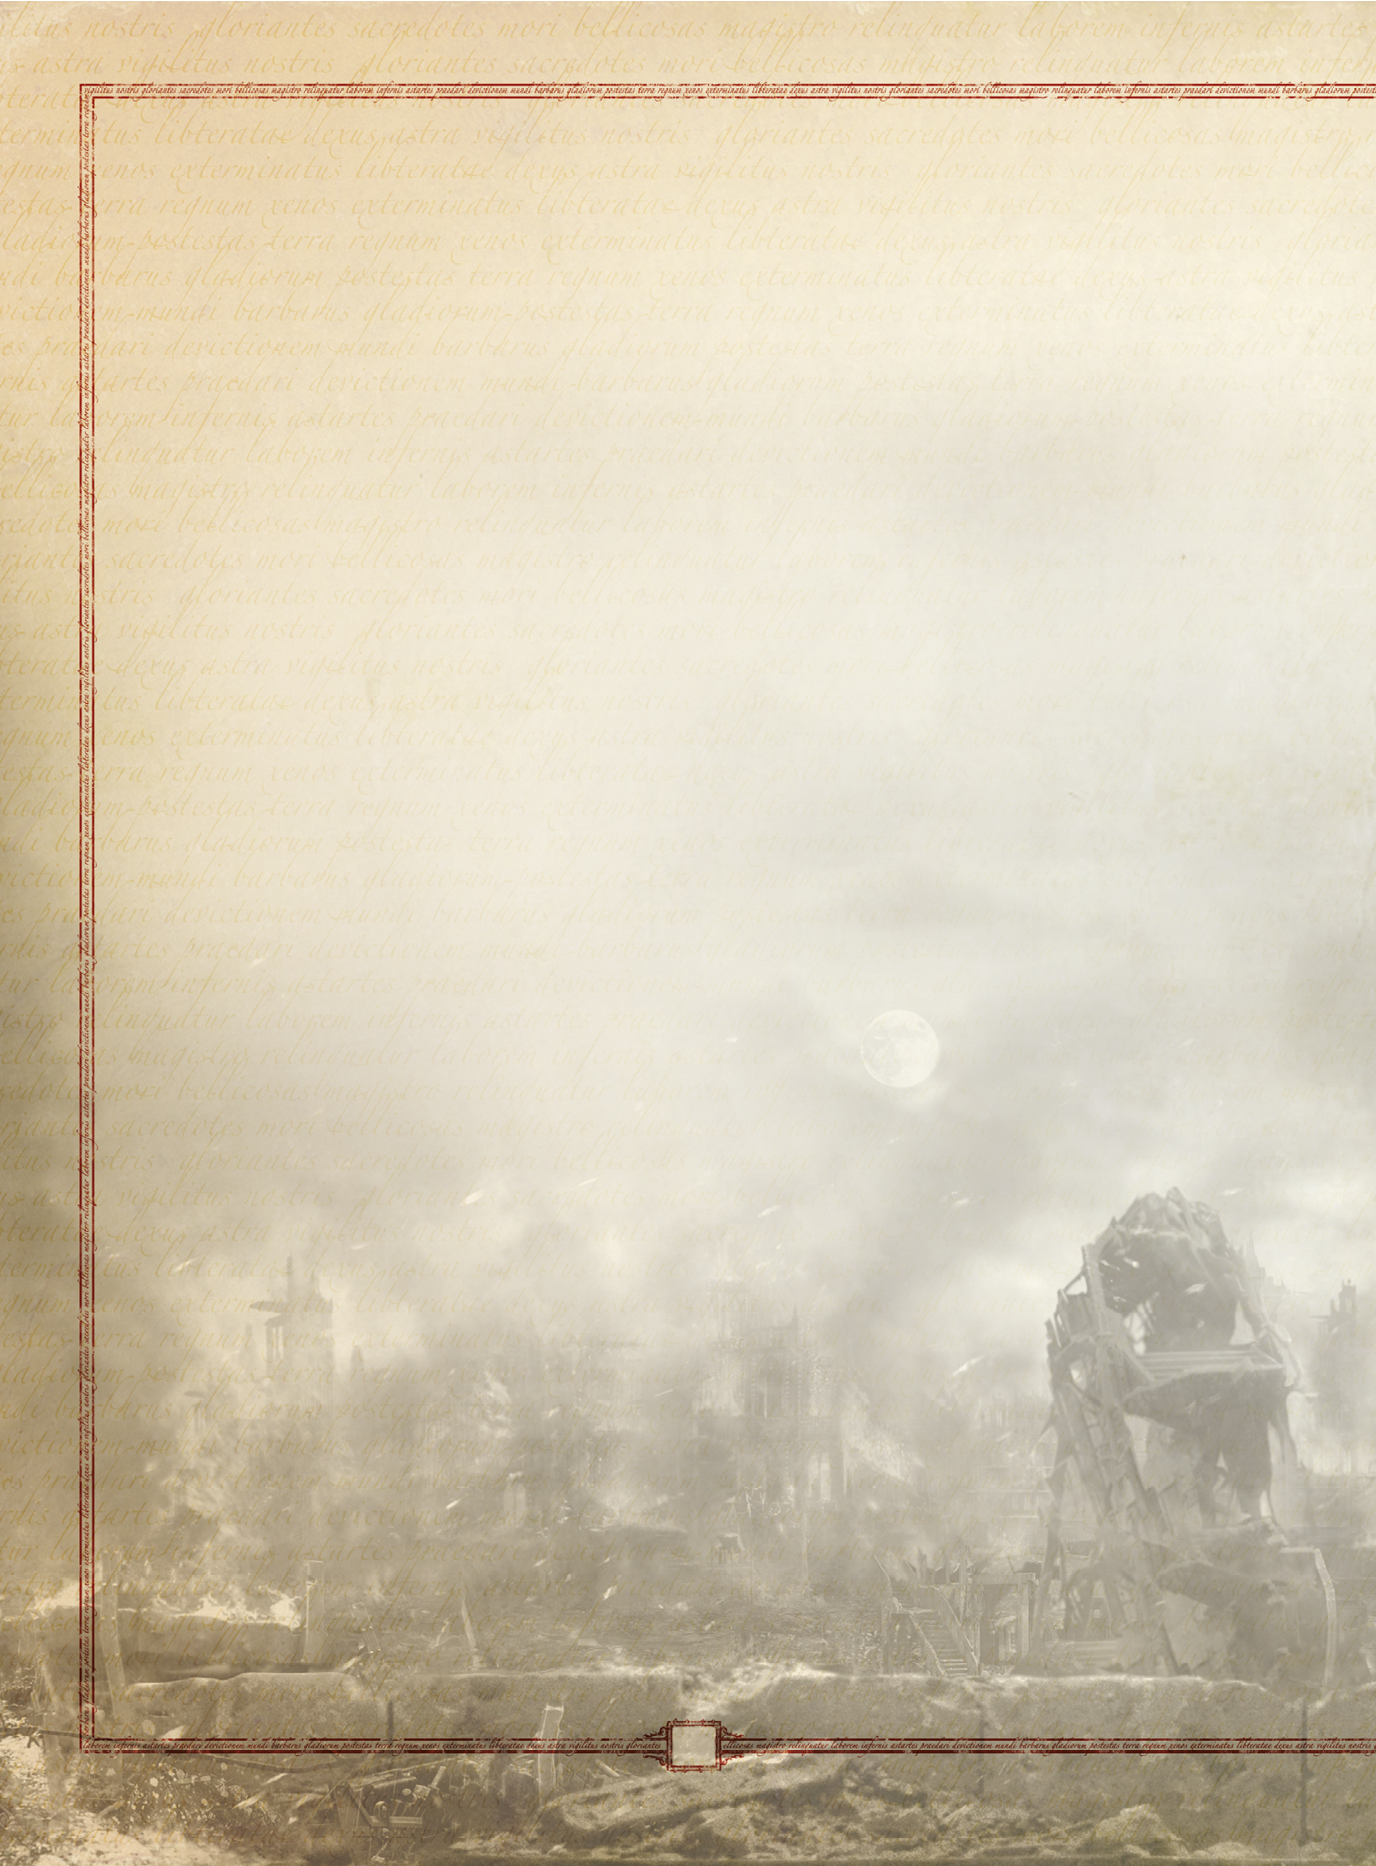
\includegraphics[width=\paperwidth,height=\paperheight]{background_left.png}
		\else
			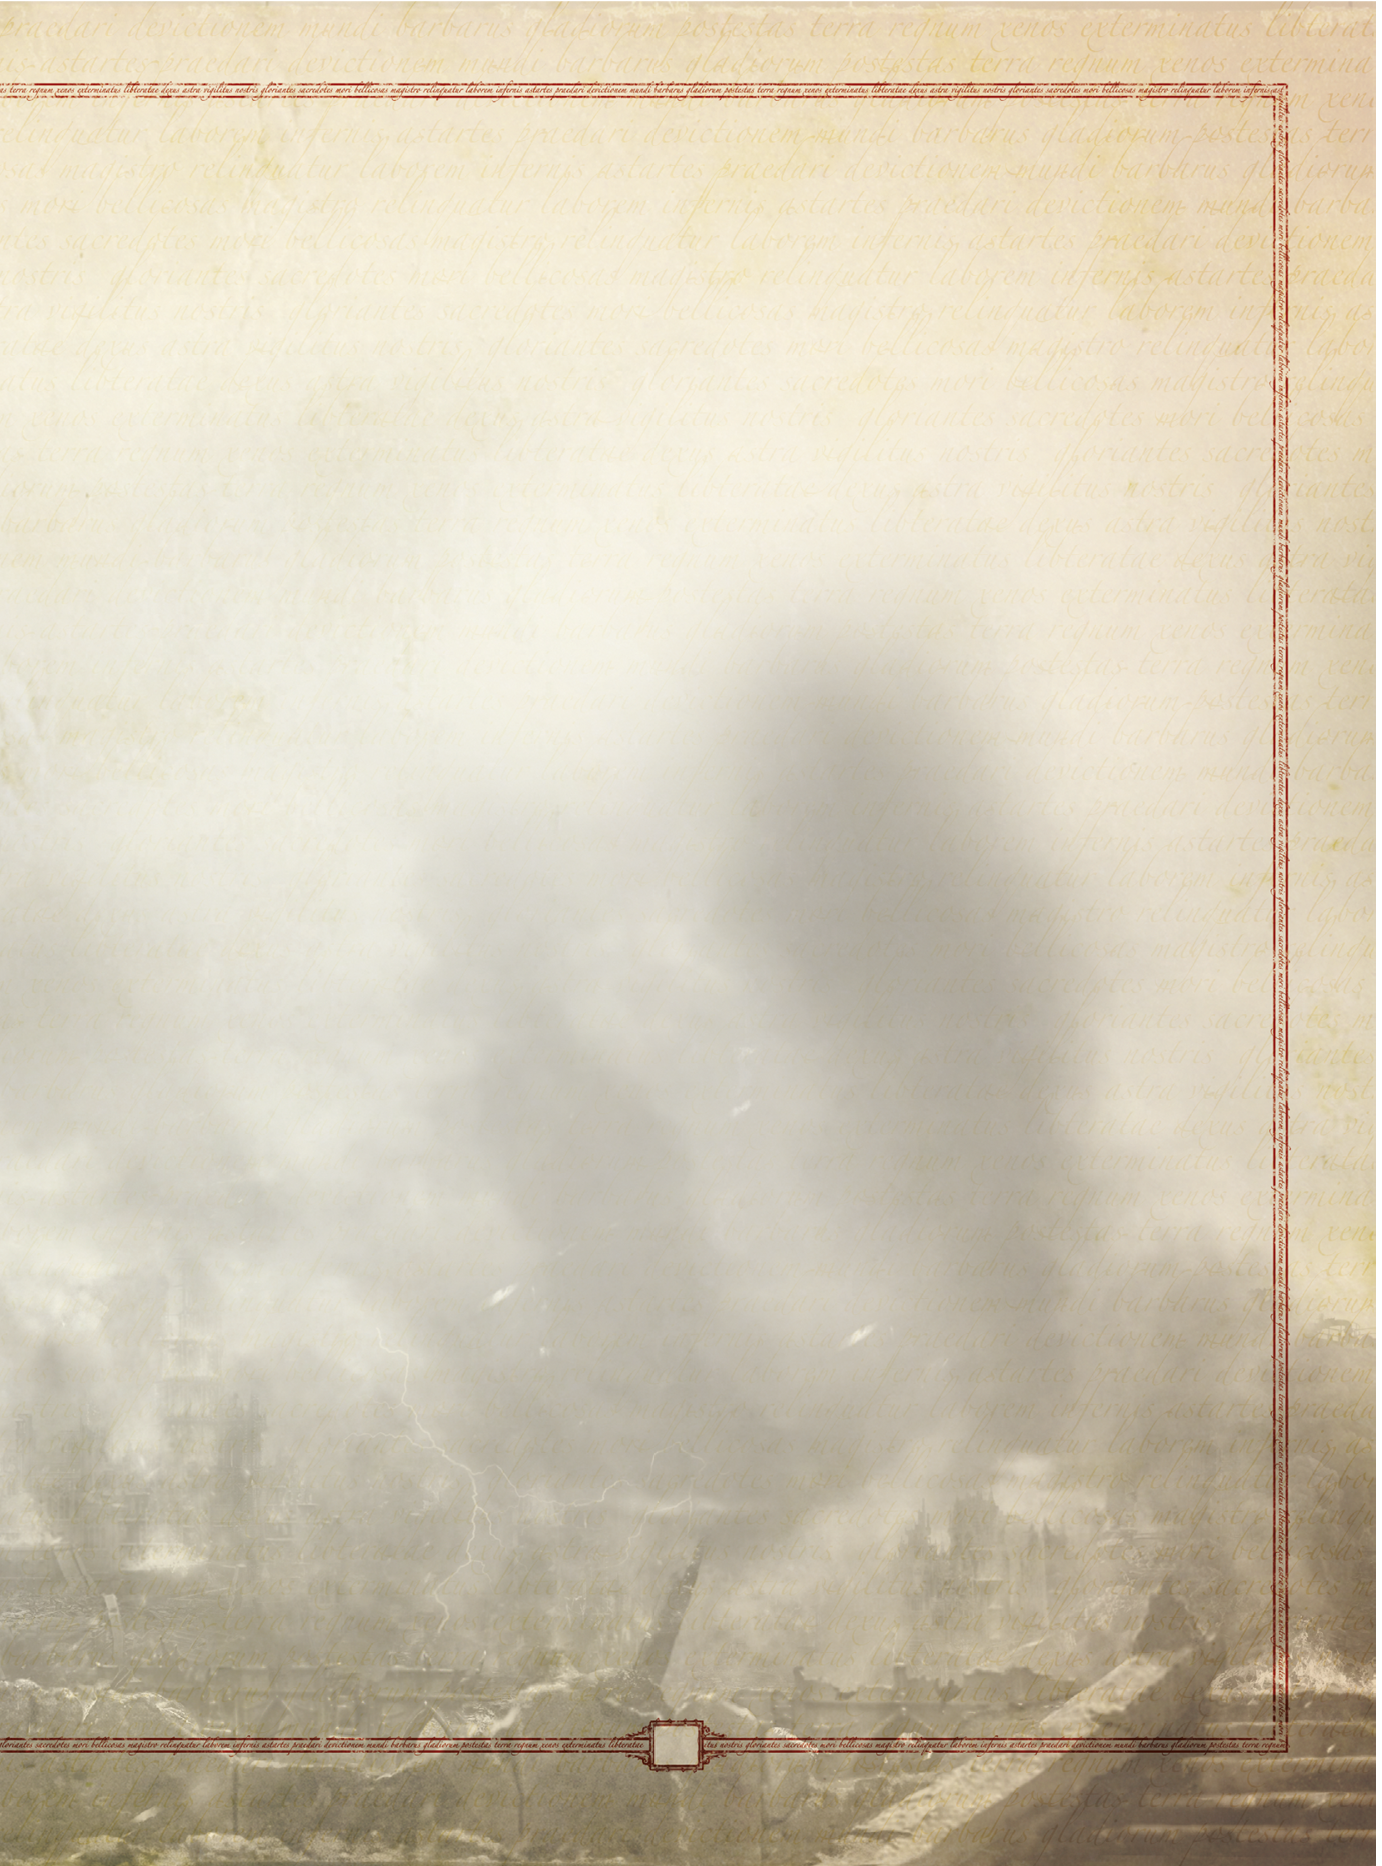
\includegraphics[width=\paperwidth,height=\paperheight]{background_right.png}		
		\fi
	}%
}

\usepackage{contour}
\usepackage{colortbl}
\usepackage{enumitem}
\usepackage{indentfirst}
\usepackage[utf8]{inputenc}
\usepackage{multicol}
\usepackage{multirow}
\usepackage{titletoc}
\usepackage[none]{hyphenat}
\usepackage{hyperref}
\usepackage{xcolor}
\usepackage{tabularx}
\usepackage{wrapfig}
\usepackage{graphics}
\usepackage{graphicx}
\usepackage{changepage}
\usepackage{wrapfig}
\usepackage[T1]{fontenc}
\usepackage{mdframed}
\usepackage{nicematrix}
\usepackage{rotating}
\usepackage{transparent}
\usepackage{threeparttable}
\usepackage{tikz}
\newcommand{\cellgray}[2]{\Block[tikz={fill=gray,opacity = .25}]{1-#1}{#2}}
\usepackage{titlesec}
%\titleformat*{\section}{%
	%	\selectfont} 
\usepackage{geometry}
\geometry{
	a4paper,
	inner=60pt,
	textwidth=520pt,
	height=710pt,
}

\usepackage{pgf}
\usepackage{pgfpages}
\pgfpagesdeclarelayout{boxed}
{
	\edef\pgfpageoptionborder{0pt}
}
{
	\pgfpagesphysicalpageoptions
	{%
		logical pages=1,%
	}
	\pgfpageslogicalpageoptions{1}
	{
		border code=\pgfsetlinewidth{1pt}\pgfstroke,%
		border shrink=\pgfpageoptionborder,%
		resized width=1.0\pgfphysicalwidth,%
		resized height=1.0\pgfphysicalheight,%
		center=\pgfpoint{.5\pgfphysicalwidth}{.5\pgfphysicalheight}%
	}%
}

\usepackage[skins,breakable]{tcolorbox}
\usepackage{paracol}

\newtcolorbox{breakbox}[1][]{%
	breakable,
	blanker
}
\newtcolorbox{section_header}[1][]{%
	enhanced jigsaw, 
	enlarge top by=-2.5cm, 
	top=2.1cm,
	interior style={top color=#1, bottom color=white}
}
\newtcolorbox{coloredbox}{breakable}

\pgfpagesuselayout{boxed}

\newcolumntype{Z}[1]{>{\arraybackslash}m{#1}}

\newcommand{\quickref}[1]{\textcolor{violet}{\hyperref[#1]{#1}}}

\renewcommand{\labelitemi}{$\vcenter{\hbox{\tiny$\bullet$}}$}

\setlist[itemize]{itemsep=-3pt, topsep=1pt}

\def\restofpage{\dimexpr\pagegoal-\pagetotal-\baselineskip\relax}
\def\dotfill{\leaders\hbox{.}\hfill}

\newsavebox\mysavebox
\newenvironment{imgminipage}[2][]{%
	\def\imgcmd{\includegraphics[width=\wd\mysavebox,height=\dimexpr\ht\mysavebox+\dp\mysavebox\relax,#1]{#2}}%
	\begin{lrbox}{\mysavebox}%
		\begin{minipage}%
		}{%
		\end{minipage}
	\end{lrbox}%
	\sbox\mysavebox{\fbox{\usebox\mysavebox}}%
	\mbox{\rlap{\raisebox{-\dp\mysavebox}{\imgcmd}}\usebox\mysavebox}%
}

\definecolor{bronze}{rgb}{.745, .659, .525}
\newcommand{\setbackground}{
	\backgroundsetup{
		scale=1,
		color=black,
		opacity=1,
		angle=0,
		contents={%
			\includegraphics[width=\paperwidth,height=\paperheight]{marble.jpg}
		}%
}
\color{bronze}}
\newcommand{\clearbackground}{
	\backgroundsetup{
		scale=1,
		color=black,
		opacity=1,
		angle=0,
		contents={%
			\checkoddpage
			\ifoddpage
			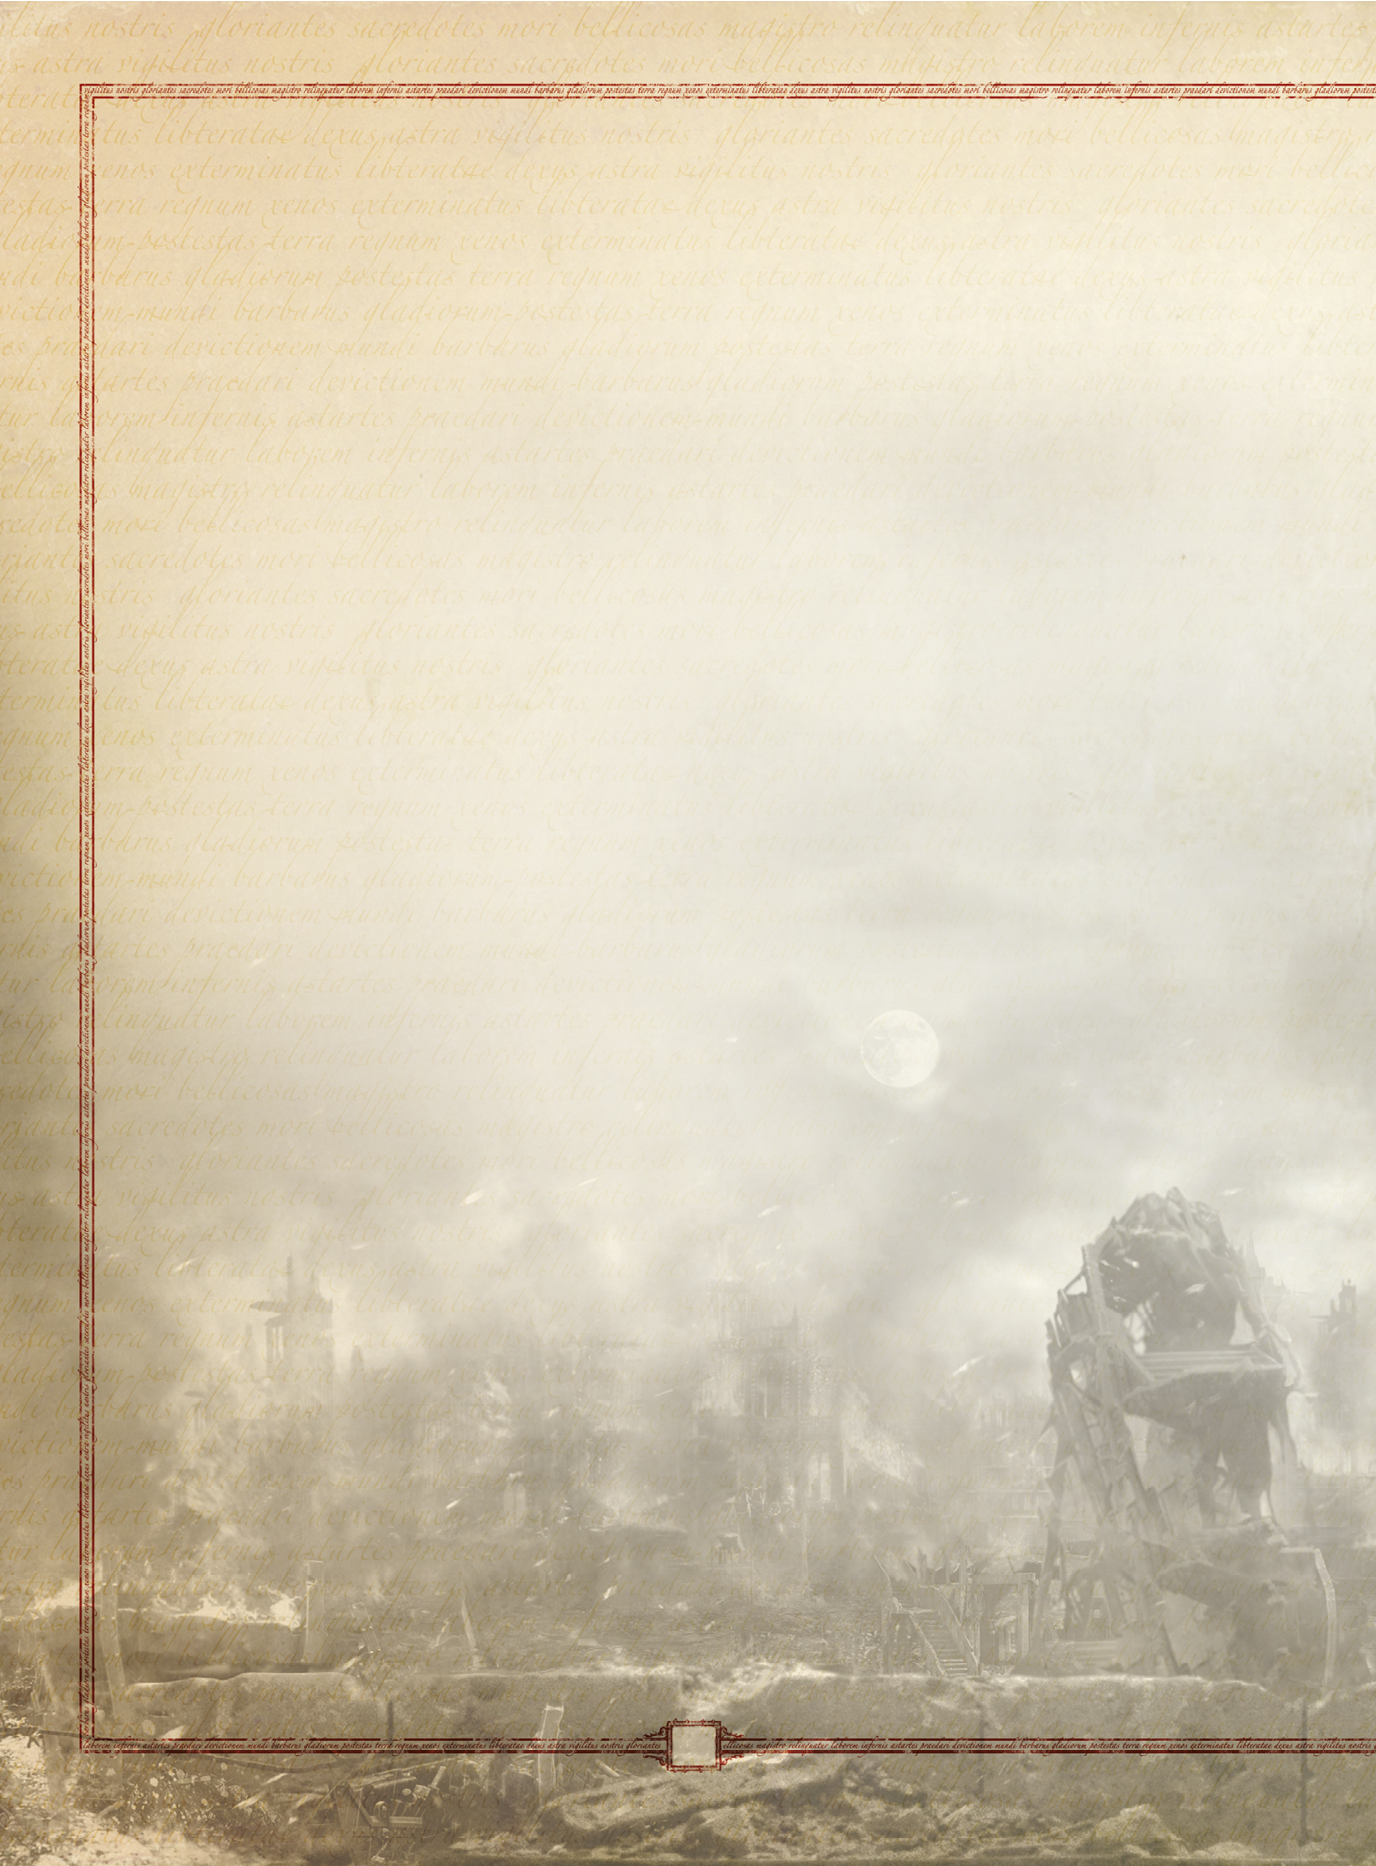
\includegraphics[width=\paperwidth,height=\paperheight]{background_left.png}
			\else
			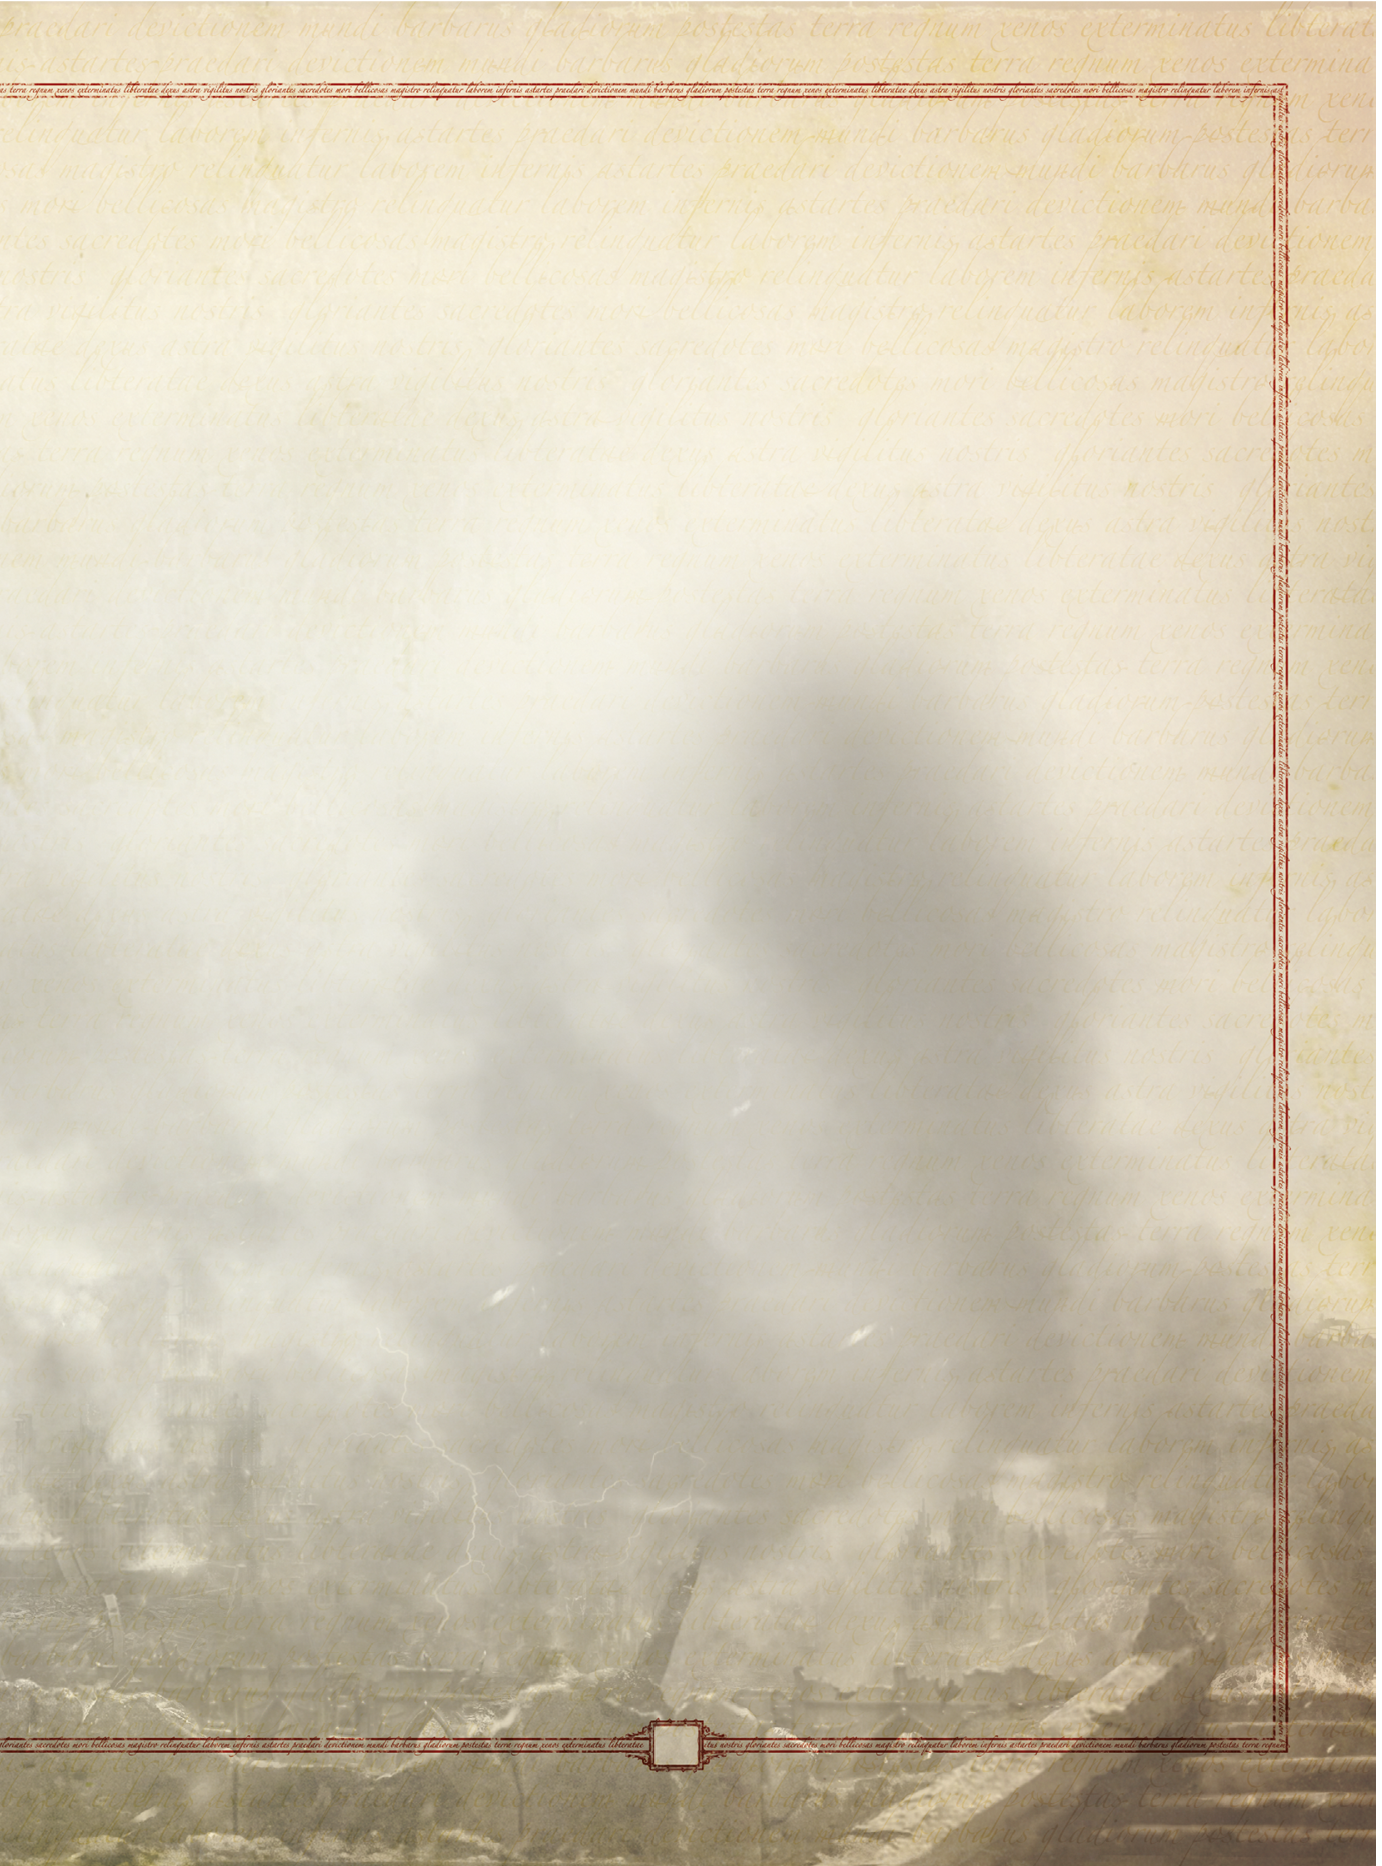
\includegraphics[width=\paperwidth,height=\paperheight]{background_right.png}		
			\fi
		}%
}
\color{black}}

% Centering the page nubmers since they're assymetric boxes on the background
\makeatletter
\def\ps@myPS{%
	\def\@oddfoot{\centering\hspace{24.6em}\thepage}
	\def\@evenfoot{\centering\hspace{28em}\thepage}%
	\def\@evenhead{\null\hfil\slshape\leftmark}%
	\def\@oddhead{{\slshape\rightmark}}}%
\makeatother
\pagestyle{myPS}

\title{Horus Heresy 2.0 Necrons}
\author{ingeanus}
\date{June 2024}

\begin{document}
	\renewcommand\thesection{}
	\renewcommand\thesubsection{}
	\renewcommand\thesubsubsection{}
	\contourlength{0.5pt} %how thick each copy is
	\contournumber{3}  %number of copies
	
	\maketitle
	
	\tableofcontents
	
	\newpage
	\section{The Necron Tombworlds}


\subsection{Building a Necron Army}

In games of the Horus Heresy: Age of Darkness, the models under a given player’s control are referred to as that player’s army. Each army is composed of a single Force Organisation chart (most commonly using the Crusade Force Organisation chart), which will include one or more Detachments. An army whose Primary Detachment is selected from any Army List is considered to have the Faction of that Primary Detachment (for example, an army whose Primary Detachment was selected from the Necrons List would be considered an Necron army). Units from various Sub-factions cannot be mixed in the same Detachment, unless a Special Rule or other ability permits this.

Other, non-Primary, Detachments in the same army may be selected from any other Army List - following any additional restrictions applied, such as the ones on the next page - but each Detachment may only include units from a single Army List, unless another Special Rule states otherwise.

When selecting a Primary Detachment, you must also choose a Sub-Faction for that detachment, in the form of a Necron Dynasty. Each Dynasty provides special bonuses and options for their units and determines the Alliance Levels between other Sub-Factions.

In addition, each Dynasty has a number of allied units that are usually attached to its Tomb Worlds, whether that be Triarch Praetorians watching over the slumbering necrons, a Destroyer Cult filling part of their ranks, or Flayed Ones lurking at the fringes. As such, a Primary Detachment is also allowed to incorporate a number of Allied Units without requiring an entire Allied Detachment be taken, so long as the number of points spent on Triarch, Destroyer, and Flayed models does not exceed 25\% of the army's total points.

\newpage
\subsection{Force Organisation Charts and Detachments}

The maximum and minimum number of units that may be included in a given army is defined by a Force Organisation chart, of which there is one basic chart available, the Crusade Force Organisation chart. 

Any Force Organisation chart is made up of one or more Detachments. A Force Organisation chart will always include one Primary Detachment, which must be selected, and may also include a number of optional Detachments which a player may choose to use or ignore. Each Detachment that a player chooses to use as part of their army must use a single Army List, which determines the Faction of that Detachment. Most optional Detachments are not required to be the same Faction as the Primary Detachment, but some Detachments may have special rules which require them to be of a certain Faction (and thus use a specific Army List). Detachments of different Factions in the same army will have additional special rules that determine how they interact (see \hyperref[allies]{the Allied Section}).

Each Detachment is composed of a number of boxes, each linked to one of the Battlefield Roles. Each of these boxes allows the player to make one selection from the section of their Army List that includes units of the same Battlefield Role. Dark boxes indicate Compulsory selections, which must be included as part of the Detachment, while the lighter boxes indicate optional choices, which are only included as part of the Detachment if the player in question chooses to do so.

Sometimes, a single choice in a Detachment may allow you to select more than one unit, or to vary the Battlefield Role of the unit selected. In all cases, such deviations from the normal procedure will be fully explained in the Force Organisation chart that the Detachment is part of.
 
Each unit selected to fill a box in any single Detachment must be chosen from the same Army List, and must be of the same Battlefield Role as that of the box. The unit profile in the Army List will dictate the number of points from the points limit that must be spent to add the unit to the player’s army. Players continue to spend points to fill boxes in Detachments within the chosen Force Organisation chart until either they run out of points, fill all boxes in all available Detachments or the player chooses to stop.

\subsection{Nodal Command Force}

The legions of a Tomb World appear to have no permanent organizational structure. Each battle, campaign and Harvest causes a specific response from the Tomb World's controlling program leading to an ever-changing chain of command. This is made possible by the Nodal Command system. A Nodal Command system allocates a hierarchy to all of the elements within it, and subsequently gives a greater operational, and decision- making, capacity to certain nodes before slaving lower ranking portions of the system to these nodes.

In battle, Necron Lords form the nodes of this structure and are assigned a hierarchical value which may change over time. As this hierarchy allows for simultaneous control of a large number of Necrons by a high ranking node, while still allowing independent reaction at the level of a Necron Warrior, it allows precise organization of the Necron force as a whole while also allowing detached groups to analyze, and react to, unforeseen situations independently.

When selecting the Nodal Command Force as your Primary Detachment, you must also determine the level at which the Tomb World is operating at. This level determines what Force Organisation slots are available to you alongside what units are considered compulsory. When selecting a higher level, you must take all of the compulsory options for that level and all levels below it. For example, selecting a Decurion Formation has a Compulsory list of: 1 HQ (Silver), 1 HQ (Bronze), 2 Troops. Compulsory units for levels above yours are \textit{not} Compulsory, you may not include any Force Organization slots above your level at all — the Tomb World has not woken up to that degree.

\subsubsection{Necron Line Formation (Bronze Command)}

The main bulk of a Necron fighting force, a Bronze level command makes up various formations led by Bronze level Lords. By themselves, these formations are usually the first coalescent response to a Tomb World's invaders, summoned when a Primary Awakener Force encounters threats too potent or complex for them to handle. 

The actual formation does vary by Tomb World and Dynasty, however each Line Formation generally contains its Bronze level Lord, a number of Phalanxes of Dynastic Warriors — or occasionally Immortals — that are supported by a small number of specialized assets such as Cyptek Conclaves, Destroyer Cults, Flayed Ones, Canopteks, and Triarch overseers, all allocated by the Tomb World and the Lord themselves.

When part of a Decurion, the usual formation is to appoint four Bronze level Lords to each Decurion, including one or more Line Formations led by the lords.

The Compulsory Headquarters unit for Necron Line Formations \textit{must} have the \quickref{Nodal Command} (Bronze) special rule.

\textbf{Primary Detachment: Necron Line Formation (Required)}
\begin{itemize}
	\item \textbf{Compulsory:} 1 HQ (Bronze),  1 Troop
	\item \textbf{Optional:} +2 Troops, +1 Elite, +2 Fast Attack, +1 Heavy Support, +4 Fortification
\end{itemize}

\subsubsection{Necron Decurion Formation (Silver Reserve Command)}

If threats are particularly potent or worthy, a high ranking or competent Lord will be appointed as Nemesor for a campaign, taking place as the overseeing Silver level Nemesor Lord for a Decurion. These oversee a number of Legions made up of Line Formations, each of which are managed by Bronze level Lords as described above. The actual Decurion is a much larger and more competent fighting force than the Line Formation Legions, with further access to superior units and specialized resources as the Tomb World is able to make them available.

As part of a greater Tesserarion, there may be one or more Decurions, however their leadership varies wildly between organizations. Some prefer to maintain a single competent Lord in control of all Decurions, while other formations call for one Silver level Lord for each Decurion.

The Compulsory Headquarters unit for Necron Decurion Formations \textit{must} have the \quickref{Nodal Command} (Silver) special rule.

\textbf{Primary Detachment: Necron Line Formation (Required)}
\begin{itemize}
	\item \textbf{Compulsory:} 1 HQ (Silver),  1 Troop
	\item \textbf{Optional:} +1 HQ, +2 Troops, +2 Elites, +1 Fast Attack, +1 Heavy Support
\end{itemize}

\subsubsection{Necron Tesserarion Formation (Gold Priority Command)}

The highest level command structure for a Necron force, it is usually led by a Tomb World's Overlord themselves after taking upon the title of Nemesor for the campaign. In particularly rare cases, this may be led by a Platinum level element in the form of a Phaeron — extremely influential and powerful Overlords that lead many worlds, even entire Dynasties — alongside his court of three Gold level Overlords chosen to direct the campaign. The Priority Command directs the Tesserarion element, fielding its largest and most powerful war machines and forces to war.

The Compulsory Headquarters unit for Necron Tesserarion Formations \textit{must} have the \quickref{Nodal Command} (Gold) special rule.

\textbf{Primary Detachment: Necron Line Formation (Required)}
\begin{itemize}
	\item \textbf{Compulsory:} 1 HQ (Gold)
	\item \textbf{Optional:} +1 HQ, +1 Phaeron, +1 Troops, +1 Elite, +1 Fast Attack, +2 Heavy Supports
\end{itemize}
 
\newpage
{
\centering
\textbf{Nodal Command Force Detachment}

\includegraphics[width=470pt, height=700pt]{Org chart.png}

\begin{figure}
	\centering
	\includegraphics[width=515pt, height=750pt]{nodal.png}
\end{figure}
}
	
	\newpage
	\usection{Necron Rules}


\usubsubsection{Awakening Protocols (Tier)} \label{Awakening Protocols}

This rule is accompanied by a tier of Bronze, Silver, Gold, and Platinum. Units with this rule can only be included in lists which contain an HQ model with the corresponding \quickref{Command Protocols} tier or lower.

\usubsubsection{Command Protocols} \label{Command Protocols}

At the start of the game, after both sides have deployed, each unit with this ability may select a Command Protocol that can be used during the game. Many options allow the player to roll a \textbf{Command Protocol check} for additional benefits. To do so, roll a Leadership Check, with success granting the listed effects. Failure causes the listed negative effect immediately.

\textbf{Protocol of Eternal Guardian}

This unit may give up their Shooting Attacks this turn to use this power during the Movement Phase. Select a single friendly Necron unit within \quickref{Nodal Range} that has not moved yet and apply one of the following affects to the unit:

\begin{itemize}
	\itemsep 0pt
	\item The chosen unit gains a 6+ Cover Save, but may not Run, until your next turn
	\item 
\end{itemize}

You may choose to make a 

\textbf{Protocol of Sudden Storm}

This unit may give up their Shooting Attacks this turn to use this power during the Movement Phase. Select a single friendly Necron unit within \quickref{Nodal Range} that has not moved yet and apply one of the following affects to the unit:

\begin{itemize}
	\itemsep 0pt
	\item The chosen unit may immediately move a number of inches up to twice its unmodified Initiative Characteristic. If the chosen unit has mixed Initiative Characteristics, use the highest unmodified Characteristics.
	\item The chosen unit ignores Difficult and Dangerous Terrain alongside negative modifiers to their movement until your next turn.
\end{itemize}

You may choose to make a Command Protocol check before using this power, if the check is successful two different options may be applied. If the Check is failed, the target unit may only move half their Movement (rounded down) this turn.

\textbf{Protocol of Vengeful Stars}

This unit may give up their Shooting Attacks this turn to use this power during the Shooting Phase. Select a single friendly Necron unit within \quickref{Nodal Range} that has not shot yet and apply one of the following affects to the unit:

\begin{itemize}
	\itemsep 0pt
	\item The chosen unit's Ranged Weapons gain the Ignores Cover rule until your next turn.
	\item The chosen unit's Ranged Weapons gain Breaching (6+) or increase the level of Breaching or Rending by 1 until your next turn.
	\item 
\end{itemize}

You may choose to make a Command Protocol check before using this power, if the check is successful two different options may be applied. If the Check is failed, the target unit suffers -1 BS this turn.

\textbf{Protocol of the Hungry Void}

This unit may give up their Shooting Attacks this turn to use this power during the Shooting Phase. Select a single friendly Necron unit within \quickref{Nodal Range} apply one of the following affects to the unit:

\begin{itemize}
	\itemsep 0pt
	\item The chosen unit gains the Hatred trait until your next turn. 
	\item The chosen unit's Melee Weapons gain Breaching (6+) or increase the level of Breaching or Rending by 1 until your next turn.
	\item 
\end{itemize}

You may choose to make a Command Protocol check before using this power, if the check is successful two different options may be applied. If the Check is failed, the target unit suffers -1 WS this turn.

\textbf{Protocol of the Undying Legions}

This unit may give up their Shooting Attacks this turn to use this power during the Shooting Phase. Select a single friendly Necron unit within \quickref{Nodal Range} and apply one of the following affects to the unit:

\begin{itemize}
	\itemsep 0pt
	\item The chosen unit can re-roll results of 1 once for \quickref{Reanimation Protocols} until next turn. Dynastic Warriors can re-rolls results of 1-2.
	\item The chosen unit's \quickref{Living Metal} ability has its It Will Not Die level increased to 3+ until next turn.
	\item 
\end{itemize}

You may choose to make a Command Protocol check before using this power, if the check is successful two different options may be applied. If the Check is failed, the target unit suffers -1 to \textit{Reanimation Protocol} rolls until next turn.

\textbf{Protocol of the Conquering Tyrant}

This unit may give up their Shooting Attacks this turn to use this power during the Movement Phase. Select a single friendly Necron unit within \quickref{Nodal Range} and apply one of the following affects to the unit:

\begin{itemize}
	\itemsep 0pt
	\item 
	\item The chosen unit gains the Hit \& Run ability until your next turn.
	\item 
\end{itemize}

You may choose to make a Command Protocol check before using this power, if the check is successful two different options may be applied. If the Check is failed, the target unit gains the Soulless Hordes (Bronze) trait this turn, if it did not already have it, and cannot ignore the Engrammatic Attack Patterns provision this turn.

\usubsubsection{Nodal Command (Tier)} \label{Nodal Command}

This rule is accompanied by a tier of Bronze, Silver, Gold, and Platinum. Each tier provides a specified range known as Nodal Range, which many other abilities reference for their effects. Additionally, any unit with the \quickref{Soulless Hordes} sub-type may ignore the Engrammatic Attack Patterns provision while within Nodal Range of a unit with this rule. The highest tier unit in your army \textit{must} be your Warlord.

\label{Nodal Range}
\begin{tabular}{|c|c|}
	\hline
	Tier & Nodal Range \\
	\hline
	Bronze & 6" \\
	Silver & 9" \\
	Gold & 12" \\
	Platinum & 12" \\
	\hline
\end{tabular}


\usubsubsection{Entropic Strike (X)} \label{Entropic Strike}

For each To Wound roll equal to or higher than the value listed, the target automatically suffers a Wound regardless of its Toughness. Against vehicles and buildings, such a hit that does not cause a Penetrating Hit automatically causes a glancing hit.

\usubsubsection{Gauss (X)} \label{Gauss}

When firing a weapon with this special rule, a To Wound roll equal to or higher than the value listed wounds automatically, regardless of the target’s Toughness. Against vehicles and buildings, an Armour Penetration roll equal to or higher than the value listed inflicts a Glancing hit. Super Heavy and Gargantuan Creatures are immune to this effect.

\usubsubsection{Living Metal} \label{Living Metal}

Infantry and Vehicles with this rule have \textbf{It Will Not Die (5+)}. Successful Wounds inflicted by attacks with the Poisoned or Fleshbane special rules must be re-rolled. The Shock Pulse affects models with this rule as well. Leadership penalties caused by the Anethema sub-type are ignored.


Vehicles ignore the effects of Crew Shaken (but still lose a Hull Point). If the vehicle is Heavy or Super-Heavy, they are not subject to the particular effects of the Lance and Melta special rules by attacks made against it.
In addition, it reduces the effects of all rolls on the Vehicle Damage chart caused by Penetrating hits (other than by Destroyer type weaponry) by -1.

\usubsubsection{Decurion/Tesserarion Nemesor} \label{Decurion Nemesor} \label{Tesserarion Nemesor}

The Decurion Nemesor / Tesserarion Nemesor special rule grants the following benefits:

\begin{itemize}
	\itemsep 0pt
	\item Rites of War: If a Detachment with the Necron Faction includes at least one model with the Decurion Nemesor special rule then that Detachment may select a single Rite of War. 
	\item Lord of the Legion: An army may only include a maximum of one model with this special rule per 1,000 points. This counts across all Detachments of an army.
	\item A model with this special rule may also include an Immortals, Pariah Lychguard, or Royal Lychguard unit as part of the same Force Organisation slot as the model with the Decurion Nemesor special rule, but must still meet the required \quickref{Awakening Protocols} tier.
\end{itemize}

If multiple units are eligible to take this ability, it can only be taken by those with the highest Nodal Command tier in the force that has not already taken this ability. 

\usubsubsection{Reanimation Protocols} \label{Reanimation Protocols}

Whenever a unit with Reanimation Protocols would suffer wounds, after the opponent's unit's attacks or the effects have been resolved and models have been removed total the number of wounds that have been lost, the unit begins \textbf{reassembling} a number of wounds equal to this amount. For each wound that is being reassembled, roll a d6, subtracting one for wounds with Instant Death. This unit \textbf{reanimates} a wound for every 5+ roll. Each time such a unit reanimates a wound:

\begin{itemize}
	\itemsep 0pt
	\item If that unit is less than its Starting Strength, return one destroyed model to play in cohesion range with one wound remaining.
	\item Then, if that unit is at its Starting Strength and has models that are missing any wounds, one of the models with the least wounds regains a wound. Controlling player decides in case of ties.
\end{itemize}

When assigning wounds to units that have multiple models missing any wounds, assign them to the models with the lowest amount of wounds. In case of ties, the attacking player decides which models to apply them to.


\usubsubsection{Soulless Hordes (X)} \label{Soulless Hordes}

Models with the Soulless Hordes subtype are subject to the Engrammatic Attack Patterns provision, which has effects dependent on the tier of the subtype:

\paragraph{Bronze:} During the controlling player's Shooting phase and Charge sub-phase, the Soulless Hordes unit must attempt a Shooting Attack if there is an enemy unit within range (they are not forced to charge), and must target the closest enemy unit possible that is within its line of sight and a valid target for a Shooting Attack or Charge. If two or more targets are equally close then the controlling player chooses which will be the target of a Shooting Attack or Charge. Similar to the Fearless rule, units with this subtype cannot use any Reactions that grant a Cover Save, Armour Save or Invulnerable Save, and cannot choose to fail a Morale check due to the Our Weapons Are Useless special rule. They additionally may not make Reactions.

\paragraph{Silver:} During the controlling player's Shooting phase and Charge sub-phase, \textit{if} the unit attempts a Shooting Attack and/or Charge they must target the closest enemy unit possible that is within its line of sight and a valid target for a Shooting Attack or Charge. If two or more targets are equally close then the controlling player chooses which will be the target of a Shooting Attack or Charge. Similar to the Fearless rule, units with this subtype cannot use any Reactions that grant a Cover Save, Armour Save or Invulnerable Save, and cannot choose to fail a Morale check due to the Our Weapons Are Useless special rule.

The \quickref{Command Protocols} trait is able to suppress this sub-type's effects while in Nodal Range.

\usubsubsection{Tesla (X)} \label{Tesla}

When firing a weapon with this special rule, a To Hit roll equal to or higher than the value listed generates an additional 2 hits. These hits may be applie to the target unit, or to any unit within 2" of the target unit.
	
	\newpage
	\section{Necron Factions}

\subsection{Charnovokh}

\textbf{Advanced Reaction:}

\textbf{Dynasty Effect:}


\subsection{Maynarkh}

Flayed One Focus. All units can take Flensing Scarabs

\textbf{Advanced Reaction:}

\textbf{Dynasty Effect:}


\subsection{Mephrit}

Shooting Focus, high firepower. Bitter Firepower reaction?

\textbf{Advanced Reaction:}

\textbf{Dynasty Effect:}


\subsection{Mephrit-Ghiar}

Like Mephrit, but should be more.. guerilla?

\textbf{Advanced Reaction:}

\textbf{Dynasty Effect:}


\subsection{Nephrekh}

\textbf{Advanced Reaction:}

\textbf{Dynasty Effect:}


\subsection{Nihilakh}

\textbf{Advanced Reaction:}

\textbf{Dynasty Effect:}


\subsection{Novokh}

Destroyer and/or melee Focus

\textbf{Advanced Reaction:}

\textbf{Dynasty Effect:}

\subsection{Sautekh}

\textbf{Advanced Reaction:}

\textbf{Dynasty Effect:}


\subsection{Szarekhan}

Some can take Master-Crafted?

\textbf{Advanced Reaction:}

\textbf{Dynasty Effect:} Maybe Stubborn?


\subsection{Thokt}

\textbf{Advanced Reaction:}

\textbf{Dynasty Effect:} Rad effect?


\subsection{Triarch}

Triarch buffs? Command buffs?

\textbf{Advanced Reaction:}

\textbf{Dynasty Effect:}


\subsection{Destroyer Cult}

Madness effect? High loss effect?

\textbf{Advanced Reaction:}

\textbf{Dynasty Effect:}


\subsection{Flayed Ones}

Anti-infantry stuff?

\textbf{Advanced Reaction:}

\textbf{Dynasty Effect:}
	
	\newpage
	\usection{Wargear}

\usubsection{Melee Weapons} \label{Melee Weapons}

\usubsubsection{Staff of Light} \label{Staff of Light}
	\noindent
	\begin{tabular}{||m{110pt} m{30pt} m{31pt} m{55pt} m{12pt} m{12pt} m{210pt}||}
		\hline
		Name & & Range & Type & S & AP & Abilities \\
		\hline
		\quickref{Staff of Light} (Shooting) & & 18" & Assault 3 & 5 & 3 & — \\
		\quickref{Staff of Light} (Melee) & & — & Melee & User & 3 & Rending (6+) \\
		\hline
\end{tabular}

\usubsubsection{Hyperphase Sword} \label{Hyperphase Sword}
\noindent
\begin{tabular}{||m{110pt} m{30pt} m{31pt} m{55pt} m{12pt} m{12pt} m{210pt}||}
	\hline
	Name & & Range & Type & S & AP & Abilities \\
	\hline
	\quickref{Hyperphase Sword} &  & — & Melee & User & 3 & Rending (5+) \\
	\hline
\end{tabular}

\usubsubsection{Voidblade} \label{Voidblade}
\noindent
\begin{tabular}{||m{110pt} m{30pt} m{31pt} m{55pt} m{12pt} m{12pt} m{210pt}||}
	\hline
	Name & & Range & Type & S & AP & Abilities \\
	\hline
	\quickref{Voidblade} &  & — & Melee & User & 4 & \quickref{Entropic Strike} (5+), Rending (6+) \\
	\hline
\end{tabular}

\usubsubsection{Voidscythe} \label{Voidscythe}
\noindent
\begin{tabular}{||m{110pt} m{30pt} m{31pt} m{55pt} m{12pt} m{12pt} m{210pt}||}
	\hline
	Name & & Range & Type & S & AP & Abilities \\
	\hline
	\quickref{Voidscythe} &  & — & Melee & x2 & 1 & \quickref{Entropic Strike} (2+), Brutal (2), Unwieldy, Two-Handed \\
	\hline
\end{tabular}

\usubsubsection{Warscythe}
\label{Warscythe}
\noindent
\begin{tabular}{||m{110pt} m{30pt} m{31pt} m{55pt} m{12pt} m{12pt} m{210pt}||}
	\hline
	Name & & Range & Type & S & AP & Abilities \\
	\hline
	\quickref{Warscythe} & x pts& — & Melee & +2 & 2 & Armourbane (Melee), Two-Handed \\
	\hline
\end{tabular}



\usubsection{Ranged Weapons} \label{Ranged Weapons}

\usubsubsection{Gauntlet Weapons}

\label{Gauntlet of Fire} \label{Tachyon Arrow}
\noindent
\begin{tabular}{||m{110pt} m{30pt} m{31pt} m{55pt} m{12pt} m{12pt} m{210pt}||}
	\hline
	Name & & Range & Type & S & AP & Abilities \\
	\hline
	\quickref{Gauntlet of Fire} & x pts& Template & Assault 1 & 4 & 5 & — \\
	\quickref{Tachyon Arrow} & x pts& 120" & Destroyer 1 & 10 & 1 & One use \\
	\hline
\end{tabular}



\usubsubsection{Gauss Weapons}

\label{Gauss Blaster} \label{Gauss Flayer} \label{Gauss Reaper} \label{Relic Gauss Blaster}
\noindent
\begin{tabular}{||m{110pt} m{30pt} m{31pt} m{55pt} m{12pt} m{12pt} m{210pt}||}
	\hline
	Name & & Range & Type & S & AP & Abilities \\
	\hline
	\quickref{Gauss Flayer} & x pts& 24" & Rapid Fire 1 & 4 & 5 & \quickref{Gauss} (6+) \\
	\quickref{Gauss Reaper} & x pts& 12" & Assault 2 & 5 & 4 & \quickref{Gauss} (6+) \\
	\quickref{Gauss Blaster} & x pts& 24" & Rapid Fire 1 & 5 & 4 & \quickref{Gauss} (6+) \\
	\quickref{Relic Gauss Blaster} & & 30" & Rapid Fire 2 & 5 & 4 & \quickref{Gauss} (6+), Master-Crafted \\	
	\hline
\end{tabular}


\usubsubsection{Tesla Weapons}
\label{Tesla Carbine}
\noindent
\begin{tabular}{||m{110pt} m{30pt} m{31pt} m{55pt} m{12pt} m{12pt} m{210pt}||}
	\hline
	Name & & Range & Type & S & AP & Abilities \\
	\hline
	\quickref{Tesla Carbine} & x pts& 24" & Assault 1 & 5 & — & \quickref{Tesla} (6+) \\	
	\hline
\end{tabular}


\usubsection{Technoarkana} \label{Technoarcana}

\paragraph*{Dispersion Shield} \label{Dispersion Shield}

Grants a 3+ Invulnerable Save, but the wielder never receives +1 Attack for fighting with two Melee weapons.

\paragraph*{Mindshackle Scarabs} \label{Mindshackle Scarabs}

When fighting in a challenge, a model with mindshackle scarabs has the Fear (1) special rule. Fear tests taken as a result of Mindshackle Scarabs must be taken on 3D6. 

\paragraph*{Phylactery} \label{Phylactery}

Increase the models It Will Not Die level to 3+.

\paragraph*{Phase Shifter} \label{Phase Shifter}

Grants a 4+ Invulnerable Save.

\paragraph*{Resurrection Orb} \label{Resurrection Orb}

Once per battle, on your turn, the bearer can activate their Resurrection Orb. If it does, select one friendly unit with \quickref{Reanimation Protocols} within \quickref{Nodal Range}. The bearer of the Orb and the selected unit immediately \textcolor{violet}{\hyperref[Reanimation Protocols]{reassembles}} a number of wounds equal to the total number of missing wounds and number of wounds from all destroyed models.

\paragraph*{Semipternal Weave} \label{Sempiternal Weave}

Increase the model's save to 2+.

\paragraph*{Tesseract Labyrinth} \label{Tesseract Labyrinth}

One use only.

The bearer can use the Tesseract Labyrinth in lieu of making a Shooting or Close Combat attack this round. Choose a unit within 6". The unit must immediately roll a Wounds Check for each model based on their current remaining wounds or be trapped within the Labyrinth while the Necron Character remains alive. Should the bearer be killed, the trapped models are immediately released from the Labyrinth and placed within 3" of where the bearer was.

This can also be used to carry a unit alongside the bearer. Select a unit to start the game inside the Tesseract Labyrinth. They can be disembarked as if they were in a Transport with no Special Abilities following the relevant rules. 

If paired with the \quickref{Mindshackle Scarabs} wargear, this can also be a unit chosen from an enemy faction. The unit is treated as a Distrusted Ally and still take up a relevent Force Org Slot. In narrative games, units that are captured at the end of the game can be included as well. Leave it your opponents as to whether it includes a Force Org Slot or points.

\usubsection{Artefacts of the Aeons} \label{Artefacts of the Aeons}

TODO: This

	
	\newpage
	\section{Cryptek Conclave Disciplines} \label{Cryptek Conclave Discipline}

When taking a Cryptek or Cryptek Lord, a \textbf{Discipline} must be taken from the list below, which grants a number of options, abilities, and restrictions to the unit.

\subsection[Harbingers of Despair ]{Harbingers of Despair  \hrulefill +5 pts}

Psychomancers must take an \quickref{Abyssal Staff} when selecting the Harbingers of Despair as their Discipline.

\subsubsection{Abyssal Staff}

\label{Abyssal Staff}
\noindent
\begin{NiceTabular}{L{115 pt} c C{40pt} *{2}{c} >{\raggedright\arraybackslash}p{240pt}}
	Name & Range & Type & S & AP & Abilities \\
	\hline
	\quickref{Abyssal Staff} &  &  &  &  & \\
	— Shooting & Template & Assault 1 & 8 & 1 & \quickref{Shroud of Despair} \\
	— Melee & — & Melee & 8 & 1 & \quickref{Shroud of Despair} \\
\end{NiceTabular}

\subsubsection[Atavindicator ]{Atavindicator  \hrulefill +20 pts}

The bearer can activate the Atavindicator at the end of their Movement: Target an enemy unit that does not have the Vehicle Unit Type within 18". The targeted unit must make a Leadership Check on 3D6. Failure causes each model in the unit to automatically hit itself with a S+1 AP — melee attack.

\subsubsection[Nightmare Shroud ]{Nightmare Shroud  \hrulefill +25 pts} 

The bearer gains the Fear (1) rule. Additionally, the Shroud may be used during the Shooting Phase instead of firing a weapon. Choose an enemy unit within 18" of the bearer. That unit must immediately take a Morale Check.

\subsubsection[Veil of Darkness ]{Veil of Darkness  \hrulefill +30 pts}

The bearer of the Veil of Darkness has the Deep Strike special rule. In addition, once per game, at the start of any friendly Movement phase, the bearer can use the Veil of Darkness to remove himself and his unit from the table, even if they are locked in combat. They then immediately arrive anywhere on the board using the rules for Deep Strike. The bearer also has the \quickref{Transpositional Defence} Advanced Reaction.



\subsection[Harbingers of Destruction ]{Harbingers of Destruction  \hrulefill +40 pts}

Plasmancers must take an \quickref{Eldritch Lance} when selecting the Harbingers of Destruction as their Discipline.

\subsubsection{Eldritch Lance}
\label{Eldritch Lance}
\noindent
\begin{NiceTabular}{L{115 pt} c C{40pt} *{2}{c} >{\raggedright\arraybackslash}p{240pt}}
	Name & Range & Type & S & AP & Abilities \\
	\hline
	\quickref{Eldritch Lance} &  &  &  &  & \\
	— Shooting & 36" & Assault 1 & 8 & 2 &Lance \\
	— Melee & — & Melee & User & 2 & Lance \\
\end{NiceTabular}

\subsubsection[Gaze of Flame]{Gaze of Flame  \hrulefill +5 pts}

Enemy units that charge this model or its unit are always treated as having a Disordered Charge.

\label{Gaze of Flame}
\noindent
\begin{NiceTabular}{L{115 pt} c C{40pt} *{2}{c} >{\raggedright\arraybackslash}p{240pt}}
	Name & Range & Type & S & AP & Abilities \\
	\hline
	\quickref{Gaze of Flame} & 8" & Assault 1  & 1 & — & Blast, Blind \\
\end{NiceTabular}

\subsubsection[Plasmic Lance]{Plasmic Lance  \hrulefill +0 pts}

Any Plasmancer may exchange their Eldritch Lance for a Plasmic Lance.

\label{Plasmic Lance}
\noindent
\begin{NiceTabular}{L{115 pt} c C{40pt} *{2}{c} >{\raggedright\arraybackslash}p{240pt}}
	Name & Range & Type & S & AP & Abilities \\
	\hline
	\quickref{Plasmic Lance} &  &  &  &  & \\
	— Shooting & 18" & Assault 3 & 7 & 2 & Armourbane (Ranged) \\
	— Melee & — & Melee & User & 2 & Armourbane (Melee) \\
\end{NiceTabular}

\subsubsection[Solar Pulse ]{Solar Pulse  \hrulefill +5 pts}

Once per game, at the start of any turn, the bearer can use this special rule. When he does, the Night Fighting rules are not in effect for the remainder of the turn (if they were in effect). In addition, when this special rule is used, enemy units targeting the bearer or his unit can only fire Snap Shots until the start of the bearer’s next turn.

\subsubsection[Quantum Orb ]{Quantum Orb  \hrulefill +5 pts}

Once per battle, at the start of your turn, the bearer can activate this item. If it does, select one point on the battlefield anywhere within 24" of the bearer and place a marker at that point. At the start of your next turn, resolve a S8 AP 3 Large Blast hit directly on that location. %TODO: Reaction?


\subsection[Harbingers of Eternity ]{Harbingers of Eternity  \hrulefill +20 pts}

Chronomancers must take an \quickref{Aeonstave} when selecting the Harbingers of Eternity as their Discipline.

\subsubsection{Aeonstave}
\label{Aeonstave}
\noindent
\begin{NiceTabular}{L{115 pt} c C{40pt} *{2}{c} >{\raggedright\arraybackslash}p{240pt}}
	Name & Range & Type & S & AP & Abilities \\
	\hline
	\quickref{Aeonstave} & — & Melee & User & — &  \quickref{Entropic Strike} (4+), Chronal Charge \\
\end{NiceTabular}

\textbf{Chronal Charge:} When a succesful To Hit roll is made with this weapon, assign it to a model before continuing, using the normal guidelines for Wound Pool allocation. At the end of this Initiative Step, this model loses the Fleet special rule and has their Weapon Skill, Ballistic Skill, Initiative and Attack values reduced to 1 for the remainder of the game. When allocating Wounds from the Wound Pool, any successful Wounds from this Weapon must be allocated to the affected model during this Fight Sub-Phase.

\subsubsection[Chronometron]{Chronometron  \hrulefill +35 pts}

A model with a Chronometron can re-roll one of its D6 rolls each phase alongside granting a 6+ Invulnerable Save. If the bearer is in a unit, this ability can be used to instead re-roll one of the units D6 rolls each phase and provides the 6+ Invulnerable Save to the attached unit as well. In addition, the bearer may make use of the \quickref{Strategical Timeweaver} Advanced Reaction.

\subsubsection[Chronotendrils]{Chronotendrils  \hrulefill +8 pts}

The bearer's movement speed increases to 9" and they gain the Hammer of Wrath (3) ability.

\subsubsection[Countertemporal Nanomines]{Countertemporal Nanomines  \hrulefill +15 pts}

Charges made against the bearer or their attached unit are always considered Disordered Charges. In addition, when measuring range between the target unit and the charging unit, consider the range as 3" longer than the actual distance during the Charge Sub-Phase.

\subsubsection[Entropic Lance]{Entropic Lance  \hrulefill +0 pts} \label{Entropic Lance}

Any Chronomancer may upgrade their Aeonstave to an Entropic Lance.

\noindent
\begin{NiceTabular}{L{115 pt} c C{40pt} *{2}{c} >{\raggedright\arraybackslash}p{240pt}}
	Name & Range & Type & S & AP & Abilities \\
	\hline
	\quickref{Entropic Lance} &  &  &  &  & \\
	— Shooting & 18" & Assault 1 & 7 & 3 & Brutal (2), \quickref{Entropic Strike} (2+) \\
	— Melee & — & Melee & User & 3 & Brutal (2), \quickref{Entropic Strike} (2+) \\
\end{NiceTabular}

\subsubsection[Timesplinter Cloak ]{Timesplinter Cloak  \hrulefill +40 pts}

A model with a Timesplinter Cloak has a 3+ Invulnerable save.


\subsection[Harbingers of Storm ]{Harbingers of Storm  \hrulefill +20 pts}

Ethermancers must take an \quickref{Voltaic Staff} when selecting the Harbingers of Storm as their Discipline.

\subsubsection{Voltaic Staff}
\label{Voltaic Staff}
\noindent
\begin{NiceTabular}{L{115 pt} c C{40pt} *{2}{c} >{\raggedright\arraybackslash}p{240pt}}
	Name & Range & Type & S & AP & Abilities \\
	\hline
	\quickref{Voltaic Staff} &  &  &  &  & \\
	— Shooting & 18" & Assault 4 & 6 & — & Haywire, \quickref{Tesla} (6+) \\
	— Melee & — & Melee & User & — & Haywire, \quickref{Tesla} (6+) \\
\end{NiceTabular}

\subsubsection[Ether Crystal ]{Ether Crystal  \hrulefill +5 pts}

Any enemy unit arriving by Deep Strike within \quickref{Nodal Range} of the bearer suffers D6 S8 AP 5 hits. If they arrive within range of multiple Crystals, only increase the number of hits by 1 for each Crystal past the first.

\subsubsection[Living Lightning ]{Living Lightning  \hrulefill +5 pts}

At the beginning of the Fight Sub-Phase, each enemy unit within \quickref{Nodal Range} of the bearer suffers a S8 AP 5 hit. TODO: Reaction?

\subsubsection[Metalodermal Tesla Weave ]{Metalodermal Tesla Weave  \hrulefill +15 pts}

When an enemy unit successfully moves into assault with the Cryptek or his unit, the assaulting unit immediately suffers D6 S8 AP 5 hits.




\subsection[Harbingers of Technomancy ]{Harbingers of Technomancy  \hrulefill +25 pts}

Technomancers must take a \quickref{Staff of Light} when selecting the Harbingers of Technomancy as their Discipline. Additionally, they must purchase the \quickref{Rites of Reanimation} ability.

\subsubsection[Canoptek Cloak ]{Canoptek Cloak  \hrulefill +5 pts}

Increase the bearer's move to 12" and it gains the Fleet (1) rule alongside the Floating and Light sub-type.

\subsubsection[Canoptek Control Node ]{Canoptek Control Node  \hrulefill +12 pts}

Double your \quickref{Nodal Range} when determining whether a friendly Necron unit with the Canoptek Sub-Type is within it. TODO: Reaction to shoot back better?

\subsubsection[Fail-Safe Overcharger ]{Fail-Safe Overcharger  \hrulefill +10 pts}

At the start of the Movement Phase, this model may give up its Shooting attacks for this turn to use this power. If you do so, make a Leadership Check. Failure causes an immediate wound to the selected unit that only Invulnerability and Damage Mitigation rolls can prevent. Success allows you to select a single friendly Necron unit with the Canoptek Sub-Type with \quickref{Nodal Range} and apply one of the following effects to that unit.

\begin{itemize}
	\item The chosen unit gains +1 BS until the end of the next turn.
	\item The chosen unit gains +1 WS until the end of the next turn.
	\item The chosen unit gains +1 A until the end of the next turn.
	\item The chosen unit gains a 6+ Invulnerability Save until the end of the next turn.
	\item The chose unit gains +3 M until the end of the next turn.
\end{itemize}

You may attempt to apply multiple options at once to the same unit or to multiple units within \quickref{Nodal Range} by taking a cumulative -1 penalty to your Leadership Check for each option after the first. The same option may be taken multiple times if selecting different units and still counts as taking multiple options. If applying options to multiple units, a failed check causes an immediate wound to each unit as described above.

\subsubsection[Phylacterine Hive ]{Phylacterine Hive  \hrulefill +5 pts}

Once per battle, when using your \quickref{Rites of Reanimation} ability, you may select a non-friendly unit with \quickref{Reanimation Protocols} (Such as Destroyer Cult or Flayer units) to be affected. When you do so, the unit also gains a +1 bonus to \quickref{Reanimation Protocols} rolls.

\subsubsection{Rites of Reanimation} \label{Rites of Reanimation}

After this model has moved, select a friendly unit with \quickref{Reanimation Protocols} within \quickref{Nodal Range} on the bearer. That unit immediately \textcolor{violet}{\hyperref[Reanimation Protocols]{reassembles}} a number of wounds equal to the number of lost wounds plus the number of wounds from all destroyed models, but roll with a -1 modifier if the unit is not a Dynastic Warriors Phalanx.



\subsection[Harbingers of Transmogrification ]{Harbingers of Transmogrification  \hrulefill +15 pts}

Geomancers and Alchemists must take an \quickref{Tremorstave} when selecting the Harbingers of Transmogrification as their Discipline.

\subsubsection{Tremorstave}
\label{Tremorstave}
\noindent
\begin{NiceTabular}{L{115 pt} c C{40pt} *{2}{c} >{\raggedright\arraybackslash}p{240pt}}
	Name & Range & Type & S & AP & Abilities \\
	\hline
	\quickref{Tremorstave} &  &  &  &  & \\
	— Shooting & 36" & Assault 1 & 4 & — & Blast, Pinning, \quickref{Quake}  \\
	— Melee & — & Melee & User & — & Pinning, \quickref{Quake} \\
\end{NiceTabular}

\subsubsection[Harp of Dissonance ]{Harp of Dissonance  \hrulefill +10 pts}

Any Geomancer or Alchemist may replace is \quickref{Tremorstave} with a \quickref{Harp of Dissonance}

\label{Harp of Dissonance}
\noindent
\begin{NiceTabular}{L{115 pt} c C{40pt} *{2}{c} >{\raggedright\arraybackslash}p{240pt}}
	Name & Range & Type & S & AP & Abilities \\
	\hline
	\quickref{Harp of Dissonance} & $\infty$ & Assault 1 & 6 & — & \quickref{Entropic Strike} (3+) \\
\end{NiceTabular}

\subsubsection[Cryptogeometric Adjuster]{Cryptogeometric Adjuster  \hrulefill +20 pts}

At the start of your Shooting Phase, select an enemy unit within 18". Until the end of your next turn, whenever that unit measures distance for Shooting attacks or Charges, treat the distance between the attacking unit and the target as 6" longer than the actual distance for Shooting Attacks and 3" longer than the actual distance for Charges.


\subsubsection[Seismic Crucible]{Seismic Crucible \hrulefill +15 pts}

At the start of your Shooting Phase, select an enemy unit within 18". Until the start of your next turn, if that unit has the Vehicle Unit-Type it treats all terrain as Difficult terrain, otherwise it treats all terrain as Difficult and Dangerous terrain.


\section{Powers of the C'tan} \label{Powers of the C'tan}

\subsection{General Powers}

\subsubsection{Antimatter Meteor} \label{Antimatter Meteor}

\noindent
\begin{NiceTabular}{L{115 pt} c C{40pt} *{2}{c} >{\raggedright\arraybackslash}p{240pt}}
	Name & Range & Type & S & AP & Abilities \\
	\hline
	\quickref{Antimatter Meteor} &  &  &  &  & \\
	— Shard & 24" & Assault 1 & 8 & 3 & Large Blast \\
	\cellgray{6}{} — Transcendent & 48" & Assault 1 & 8 & 3 & Apocalyptic Blast \\
\end{NiceTabular}

\subsubsection{Cosmic Fire} \label{Cosmic Fire}

\noindent
\begin{NiceTabular}{L{115 pt} c C{40pt} *{2}{c} >{\raggedright\arraybackslash}p{240pt}}
	Name & Range & Type & S & AP & Abilities \\
	\hline
	\quickref{Cosmic Fire} &  &  &  &  & \\
	— Shard & Template & Assault 1 & 6 & 4 & Torrent (24") \\
	\cellgray{6}{} — Transcendent & Template & Assault 2 & 6 & 4 & Torrent (36") \\
\end{NiceTabular}

\subsubsection{Entropic Touch} \label{Entropic Touch}

The C'tan's weapons and powers gain the \quickref{Entropic Strike} trait at a level dependent on the Power's Level.

\textbf{Shard:} \quickref{Entropic Strike} (4+)

\textbf{Transcendent:} \quickref{Entropic Strike} (1+). In addition, this ignores all rules that prevent lowering of Saves or Armour Values.

\subsubsection{Moulder of Worlds} \label{Moulder of Worlds}

\noindent
\begin{NiceTabular}{L{115 pt} c C{40pt} *{2}{c} >{\raggedright\arraybackslash}p{240pt}}
	Name & Range & Type & S & AP & Abilities \\
	\hline
	\quickref{Moulder of Worlds} &  &  &  &  & \\
	— Shard & 24" & Assault 3 & 4 & 5 & Massive Blast, Pinning, Shell Shock (1) \\
	\cellgray{6}{} — Transcendent & 48" & Assault 6 & 4 & 5 & Apocalyptic Blast, Pinning, Shell Shock (1) \\
\end{NiceTabular}

\subsubsection{Pyreshards} \label{Pyreshards}

\noindent
\begin{NiceTabular}{L{115 pt} c C{40pt} *{2}{c} >{\raggedright\arraybackslash}p{240pt}}
	Name & Range & Type & S & AP & Abilities \\
	\hline
	\quickref{Pyreshards} &  &  &  &  & \\
	— Shard & 18" & Assault 8 & 5 & — & Armourbane (Melta) \\
	\cellgray{6}{} — Transcendent  & 36" & Assault 16 & 5 & — & Armourbane (Melta) \\
\end{NiceTabular}

\subsubsection{Sentient Singularity} \label{Sentient Singularity}

All terrain within a number of inches, dependent on the Power's Level, of the C'tan is treated as Difficult and Dangerous Terrain for enemy units. Additionally, Deep Striking enemy units arriving within range are automatically considered Disordered.

\textbf{Shard:} 6"

\textbf{Transcendent:} 12"

\subsubsection{Seismic Assault} \label{Seismic Assault}

\noindent
\begin{NiceTabular}{L{115 pt} c C{40pt} *{2}{c} >{\raggedright\arraybackslash}p{240pt}}
	Name & Range & Type & S & AP & Abilities \\
	\hline
	\quickref{Seismic Assault} &  &  &  &  & \\
	— Shard & 24" & Assault 10 & 6 & 4 & Pinning, \quickref{Quake} \\
	\cellgray{6}{} — Transcendent & 48" & Assault 20 & 6 & 4 & Pinning, \quickref{Quake} \\
\end{NiceTabular}

\subsubsection{Sky of Falling Stars} \label{Sky of Falling Stars}

\noindent
\begin{NiceTabular}{L{115 pt} c C{40pt} *{2}{c} >{\raggedright\arraybackslash}p{240pt}}
	Name & Range & Type & S & AP & Abilities \\
	\hline
	\quickref{Sky of Falling Stars} &  &  &  &  & \\
	— Shard  & 24" & Assault 3 & 7 & 4 & Barrage, Large Blast \\
	\cellgray{6}{} — Transcendent & 48" & Assault 6 & 7 & 4 & Apocalyptic Barrage \\
\end{NiceTabular}

\subsubsection{Swarm of Spirit Dust} \label{Swarm of Spirit Dust}

The C'tan gains Shrouded at a level dependent on the Power's Level. Additionally, when targeted by a Shooting Attack, the range between an attacking unit and this model is considered to be a number of inches longer than actual, dependent on the Power's Level. In addition, when attacked by a weapon with the Barrage special rule a unit including one or more models with a distort field is always treated as though it was out of line of sight when scattering any attacks.

\textbf{Shard:} Shrouded (6+), +6"

\textbf{Transcendent:} Shrouded (5+), +9"

\subsubsection{Time's Arrow} \label{Time's Arrow}

\noindent
\begin{NiceTabular}{L{115 pt} c C{40pt} *{2}{c} >{\raggedright\arraybackslash}p{240pt}}
	Name & Range & Type & S & AP & Abilities \\
	\hline
	\quickref{Time's Arrow} &  &  &  &  & \\
	— Shard & 24" & Destroyer 1 & 10 & 1 & Precision Shot (6+) \\
	\cellgray{6}{} — Transcendent & 48" & Destroyer 2 & 10 & 1 & Precision Shot (5+) \\
\end{NiceTabular}

\subsubsection{Transdimensional Thunderbolt} \label{Transdimensional Thunderbolt}

\noindent
\begin{NiceTabular}{L{115 pt} c C{40pt} *{2}{c} >{\raggedright\arraybackslash}p{240pt}}
	Name & Range & Type & S & AP & Abilities \\
	\hline
	\quickref{Transdimensional Thunderbolt} &  &  &  &  & \\
	— Shard & 24" & Assault 1 & 9 & 1 & Tesla (6+) \\
	\cellgray{6}{} — Transcendent & 48" & Assault 2 & 9 & 1 & Tesla (5+) \\ & 48" & Assault 2 & 9 & 1 & Tesla (5+) \\
\end{NiceTabular}


\subsubsection{Withering Worldscape} \label{Withering Worldscape}

Whilst the C'tan Shard is on the battlefield, all Difficult terrain is Dangerous for the enemy. If the terrain is already Dangerous, the Dangerous Terrain test is failed on a 1 or a 2.


\subsection{Transcendent Powers}

\subsubsection{Seismic Shockwave} \label{Seismic Shockwave}

The C'tan's weapons gain the Reaping Blows (4) special rule.

\subsubsection{Storm of Heavenly Fire} \label{Storm of Heavenly Fire}

At the end of the C'tan's Movement phase, place a Large Blast marker centered over the model. All models under the marker (friend and foe, other than the C'tan) immediately suffer a single Strength 6 AP 3 hit with the Ignores Cover special rule.

\subsubsection{Transdimensional Maelstrom} \label{Transdimensional Maelstrom}

\noindent
\begin{NiceTabular}{L{115 pt} c C{40pt} *{2}{c} >{\raggedright\arraybackslash}p{240pt}}
	Name & Range & Type & S & AP & Abilities \\
	\hline
	\quickref{Transdimensional Maelstrom} &  &  &  &  & \\
	— Transcendent & 36" & Heavy 1 & — & — & Large Blast, Vortex \\
\end{NiceTabular}

\subsubsection{Transliminal Slide} \label{Transliminal Slide}

Instead of moving normally, the C'tan can choose to move 18" in a straight line, ignoring intervening models and terrain. Any models passed over (fried or foe) suffer a Strength 6 AP — Destroyer hit. The C'tan cannot charge in the same turn it uses this ability.

\subsubsection{Wave of Withering} \label{Wave of Withering}

\noindent
\begin{NiceTabular}{L{115 pt} c C{40pt} *{2}{c} >{\raggedright\arraybackslash}p{240pt}}
	Name & Range & Type & S & AP & Abilities \\
	\hline
	\quickref{Wave of Witheringelstrom} &  &  &  &  & \\
	— Transcendent & Hellstorm & Destroyer 1 & 9 & 1 & — \\
\end{NiceTabular}

\subsection{Specialist Powers}

\subsubsection{Gaze of Death} \label{Gaze of Death}

In its Shooting phase this model can target one non-vehicle enemy unit within 12" to which it has line of sight. Roll a number of dice determined by the Power's level: at Shard level, roll 3D6; at Transcendent level, roll 4D6. The enemy unit suffers a number of wounds equal to this total minus their Leadership. These are resolved at AP2 and with the Ignores Cover special rule. If at least one unsaved Wound is inflicted, the C’tan immediately regains one Wound lost earlier in the battle.

\subsubsection{Lord of Fire (X)} \label{Lord of Fire}

All weapons with the Flame type (as well as Heat Rays and Inferno Cannons and any other weapons which is described as using 'flame' or 'fire' as its effect or in its special rules), Melta type, and Vokite type fired within 12" of the C'tan have a chance of exploding. 

Roll a D6 each time such a weapon is fired within range. On a roll equal or greater to an amount dependent on this Power's Level, the weapon detonates. If carried by a non-vehicle model, the model immediately suffers a single Wound with an AP value equal to that of the weapon that was used to attack (Armour Saves, Invulnerable Saves and Feel No Pain rolls can be taken, but not Cover Saves or Shrouded rolls) – this Wound cannot be allocated to any other model in the unit. A Vehicle instead rolls an additional D6. If this roll results in a 1 or 2, the Vehicle suffers a Glancing Hit.

In addition, weapons of these types can never cause Wounds to a model with this special rule.

\textbf{Shard:} Lord of Fire (6+)

\textbf{Transcendent:} Lord of Fire (5+)


\subsubsection{Gaze of the Abyss} \label{Gaze of the Abyss}

If this model would be targeted by a Shooting Attack or Charge, the attacking unit must immediately make a Morale Test. Additionally, the C'tan has the Fear ability at a level dependent on this Power's Level.

\textbf{Shard:} Fear (2)

\textbf{Transcendent:} Fear (3)


\subsubsection{Grand Illusion} \label{Grand Illusion}

After all forces have been deployed and all Scout moves have been made, roll a dice dependent on the Power's Level: a D3 for Shard and D6 for Transcendent. You can immediately redeploy this many units, subject to the normal deployment rules for the mission. This power can be used to move units into or out of, reserve.


\subsubsection{Voltaic Storm} \label{Voltaic Storm}

After this model has completed its movement, target an enemy Vehicle, Dreadnought, or Automata unit within 18" with this power. Roll a D6 to determine the effect, dependent on the Power's Level.

\begin{NiceTabular}{C{10pt} p{450pt}}
	\multicolumn{2}{c}{Shard} \\
	\cellgray{2}{} D6 & Result \\
	\hline
	1 & No Effect \\
	\cellgray{2}{} 2-3 & A Vehicle Unit Type that is part of the target unit suffers 1 Glancing Hit. Any other model suffers 1 Wound. Only Invulnerable Saves or Damage Mitigation rolls may be taken against these. \\
	4-5 &  A Vehicle Unit Type that is part of the target unit suffers 1 Penetrating Hit. Any other model suffers 1 Wound. No Saves or Damage Mitigation rolls may be taken against Penetrating Hits or Wounds inflicted by this result. Re-roll results of Crew Stunned and Explodes. \\
	\cellgray{2}{} 6 &  A Vehicle Unit Type that is part of the target unit suffers 1 Penetrating Hit. Any other model suffers 1 Wound. No Saves or Damage Mitigation rolls may be taken against Penetrating Hits or Wounds inflicted by this result. \\
\end{NiceTabular}

\vspace*{2em}
\begin{NiceTabular}{C{10pt} p{450pt}}
	\multicolumn{2}{c}{Transcendent} \\
	\cellgray{2}{} D6 & Result \\
	\hline
	1 & No Effect \\
	\cellgray{2}{} 2-3 & A Vehicle Unit Type that is part of the target unit suffers 2 Glancing Hits. Any other model suffers 2 Wounds. Only Invulnerable Saves or Damage Mitigation rolls may be taken against these. \\
	4-5 &  A Vehicle Unit Type that is part of the target unit suffers 2 Penetrating Hits. Any other model suffers 2 Wounds. No Saves or Damage Mitigation rolls may be taken against Penetrating Hits or Wounds inflicted by this result. Re-roll results of Crew Stunned and Explodes. \\
	\cellgray{2}{} 6 &  A Vehicle Unit Type that is part of the target unit suffers 2 Penetrating Hits. Any other model suffers 2 Wounds. No Saves or Damage Mitigation rolls may be taken against Penetrating Hits or Wounds inflicted by this result. \\
\end{NiceTabular}

\subsection{C'tan Special Rules}

\subsubsection{Drain Life} \label{Drain Life}

Damage Mitigation rolls cannot be taken for wounds caused by this model.

\subsubsection{Flaming Vessel} \label{Flaming Vessel}

At the start of the Fight sub-phase, center a 5" Large Blast Template on this model. Each unit, except for the C'tan, suffers a S6 AP 5 Armourbane (Melta) hit for each model underneath the template.
 
\subsubsection{Matter Absorption} \label{Matter Absorption}

At the end of the turn, if an enemy Vehicle or Dreadnought was destroyed as a result of an attack made by this model, the Void Dragon immediately make a check against this model's It Will Not Die ability for each model destroyed. If successful, it regains a lost Wound and remove any wrecks for the respective vehicle from play.

\subsubsection{Misdirection} \label{Misdirection}

Attacks made against this model suffer a -1 penalty to BS and WS. When targeted by a Shooting Attack, the range between an attacking unit and this unit is considered to be 6" further than the actual range between the two units In addition, when attacked by a weapon with the Barrage special rule, this model is always treated as thought it was out of light of sight when scattering any attacks.

\subsubsection{Unfathomable Horror} \label{Unfathomable Horror}

When an enemy unit is called to take a Morale test caused by this model, enemy models with the Fearless special rule are treated as instead having the Stubborn special rule, and enemy models with the Stubborn special rule are treated as not having that special rule.

\section[Reactions]{\superhuge{Reactions}}

\subsection{Ethereal Interception} \label{Ethereal Interception}

If this unit is in Deep-Strike reserves, this reaction may be made after an enemy units arrives from Reserves and has finished all of their movement. The reacting unit immediately arrives from Reserves, following the rules for Deep Strike Assaults. Then, if it within Line of Sight of the triggering unit, it may make a Shooting attack against the triggering unit. This reaction may only be used once per turn for each unit with it. \\

\subsection{Strategical Timeweaver} \label{Strategical Timeweaver}

When an opponent declares a Shooting Attack or Fights this unit or a unit it is attached to, this reaction may be declared. The triggering unit must re-roll all successful To Hit and To Wound rolls against the reacting unit until the end of the attack, keeping the second result. This re-roll occurs even if the triggering unit's rules (e.g. Shred, Hatred, etc.) have already re-rolled these dice. This reaction may only be used once per game for each unit that is able to make use of this reaction.


	
	\newpage
	\setbackground
	\section[Units]{\texorpdfstring{\centering\Huge Units}{Units}}
	\clearbackground
	\subsection{Headquarters}

\newpage
\subsubsection[Lord]{}

\fbox{\begin{imgminipage}{marble.jpg}[t]{0.2\textwidth}
		\color{white}
		\centering {\large HQ}
		
		\raggedright \small
		\color{black}
\end{imgminipage}}
\hspace{0.5em}
\begin{minipage}[t]{0.72\textwidth}
	{\large \textbf{Lord \dotfill 30 Points}}
	
	\begin{tabular}{m{165 pt} *{10}{c}}
		& M & WS & BS & S & T & W & I & A & Ld & Sv \\
		\hline
		Lord & 7 & 4 & 4 & 5 & 5 & 2 & 2 & 2 & 10 & 3+ \\
	\end{tabular}
	\small
	\begin{minipage}{0.5\textwidth}
		\vspace*{2em}
		\textbf{Unit Composition}
		\begin{itemize}
			\item 1 Lord
		\end{itemize}
		
		\textbf{Wargear}
		\begin{itemize}
			\item \quickref{Staff of Light}
		\end{itemize}
	\end{minipage}
	\begin{minipage}{0.5\textwidth}
		\vspace*{2em}
		\textbf{Unit Type}
		\begin{itemize}
			\item Infantry (Character, Noble, \quickref{Living Metal})
		\end{itemize}
		
		\textbf{Special Rules}
		\begin{itemize}
			\item \quickref{Command Protocols}
			\item \quickref{Nodal Command} (Bronze)
			\item \quickref{Reanimation Protocols}
		\end{itemize}
	\end{minipage}
	
	\vspace*{2em}
	\textbf{Weapons}
	
	\begin{tabular}{m{95 pt} *{4}{c} >{\raggedright\arraybackslash}p{130pt}}
		& Range & Type & S & AP & Abilities \\
		\hline
		\quickref{Staff of Light} & & &  &  &  \\
		— Shooting & 18" & Assault 3 & 5 & 3 & — \\
		— Melee & — & Melee & User & 3 & Rending (6+) \\
		\quickref{Hyperphase Sword} & — & Melee & User & 3 & Rending (5+) \\
		\quickref{Voidblade} & — & Melee & User & 4 & \quickref{Entropic Strike} (4+), Rending(6+) \\
		\quickref{Warscythe} & — & Melee & +2 & 2 & Armourbane (Melee), Two-Handed \\
		\quickref{Relic Gauss Blaster} & 30" & Rapid Fire 2 & 5 & 4 & \quickref{Gauss} (6+), Master-Crafted \\
	\end{tabular}
	
	\vspace*{2em}
	\textbf{Options}
	\begin{itemize}
		\item The Lord may exchange their \quickref{Staff of Light} for one of the following options:
		\begin{itemize}			
			\item \quickref{Hyperphase Sword} \dotfill -2 points
			\item \quickref{Voidblade} \dotfill +0 points
			\item \quickref{Warscythe} \dotfill +20 points
			\item \quickref{Warscythe} with in-built \quickref{Relic Gauss Blaster} \dotfill +30 points
		\end{itemize}
		\item The Lord may take any of the following options:
		\begin{itemize}
			\item \quickref{Gauntlet of Fire} \dotfill +10 points
			\item \quickref{Tachyon Arrow} \dotfill +50 points
			\item \quickref{Mindshackle Scarabs} \dotfill +20 points
			\item \quickref{Phase Shifter} \dotfill +25 points
			\item \quickref{Phylactery} \dotfill +10 points
			\item \quickref{Resurrection Orb} \dotfill +25 points
			\item \quickref{Translocation Shroud} \dotfill +10 points
		\end{itemize}
		\item The Lord may take equipment from the \quickref{Artefacts of the Aeons} list.
	\end{itemize}
\end{minipage}



\newpage
\subsubsection[Nemesor Lord]{}

\begin{minipage}[t]{0.72\textwidth}
	{\large \textbf{Nemesor Lord \dotfill 50 points}}
	
	\begin{tabular}{m{165 pt} *{10}{c}}
		& M & WS & BS & S & T & W & I & A & Ld & Sv \\
		\hline
		Nemesor Lord & 7 & 5 & 4 & 5 & 5 & 3 & 2 & 3 & 10 & 3+ \\
	\end{tabular}
	\small
	\begin{minipage}{0.5\textwidth}
		\vspace*{2em}
		\textbf{Unit Composition}
		\begin{itemize}
			\item 1 Nemesor Lord
		\end{itemize}
		
		\textbf{Wargear}
		\begin{itemize}
			\item \quickref{Staff of Light}
		\end{itemize}
	\end{minipage}
	\begin{minipage}{0.5\textwidth}
		\vspace*{2em}
		\textbf{Unit Type}
		\begin{itemize}
			\item Infantry (Character, Noble, \quickref{Living Metal})
		\end{itemize}
		
		\textbf{Special Rules}
		\begin{itemize}
			\item \quickref{Command Protocols}
			\item \quickref{Nodal Command} (Silver)
			\item \quickref{Reanimation Protocols}
			\item \quickref{Decurion Nemesor}
		\end{itemize}
	\end{minipage}
	
	\vspace*{2em}
	\textbf{Weapons}
	
	\begin{tabular}{m{95 pt} *{4}{c} >{\raggedright\arraybackslash}p{130pt}}
		& Range & Type & S & AP & Abilities \\
		\hline
		\quickref{Staff of Light} & & &  &  &  \\
		— Shooting & 18" & Assault 3 & 5 & 3 & — \\
		— Melee & — & Melee & User & 3 & Rending (6+) \\
		\quickref{Hyperphase Sword} & — & Melee & User & 3 & Rending (5+) \\
		\quickref{Voidblade} & — & Melee & User & 4 & \quickref{Entropic Strike} (4+), Rending(6+) \\
		\quickref{Warscythe} & — & Melee & +2 & 2 & Armourbane (Melee), Two-Handed \\
		\quickref{Relic Gauss Blaster} & 30" & Rapid Fire 2 & 5 & 4 & \quickref{Gauss} (6+), Master-Crafted \\
		\quickref{Rod of Night} & & &  &  &  \\
		— Shooting & 18" & Assault 2 & 5 & — & Haywire, \quickref{Tesla} (6+) \\
		— Melee & — & Melee & User & — & \quickref{Energy Siphon}, Haywire \\
	\end{tabular}
	
	\vspace*{2em}
	\textbf{Options}
	\begin{itemize}
		\item The Nemesor Lord may exchange their \quickref{Staff of Light} for one of the following options:
		\begin{itemize}			
			\item \quickref{Hyperphase Sword} \dotfill -2 points
			\item \quickref{Rod of Night} \dotfill +5 points
			\item \quickref{Voidblade} \dotfill +0 points
			\item \quickref{Warscythe} \dotfill +20 points
			\item \quickref{Warscythe} with in-built \quickref{Relic Gauss Blaster} \dotfill +30 points
		\end{itemize}
		\item A Nemesor Lord without a Two-Handed weapon may take the following:
		\begin{itemize}
			\item \quickref{Dispersion Shield} \dotfill +30 points
		\end{itemize}
		\item The Nemesor Lord may take any of the following options:
		\begin{itemize}
			\item \quickref{Gauntlet of Fire} \dotfill +10 points
			\item \quickref{Tachyon Arrow} \dotfill +50 points
			\item \quickref{Mindshackle Scarabs} \dotfill +20 points
			\item \quickref{Phase Shifter} \dotfill +25 points
			\item \quickref{Phylactery} \dotfill +10 points
			\item \quickref{Resurrection Orb} \dotfill +25 points
			\item \quickref{Sempiternal Weave} \dotfill +10 points
			\item \quickref{Tesseract Labyrinth} \dotfill +100 points
			\item \quickref{Translocation Shroud} \dotfill +10 points
		\end{itemize}
		\item The Nemesor Lord may take equipment from the \quickref{Artefacts of the Aeons} list.
	\end{itemize}
\end{minipage}
\hspace{0.5em}
\fbox{\begin{imgminipage}{marble.jpg}[t]{0.2\textwidth}
	\color{white}
	\centering {\large HQ}
	
	\raggedleft \small
	\color{black}
\end{imgminipage}}



\newpage
\subsubsection[Nemesor Overlord]{}

\fbox{\begin{imgminipage}{marble.jpg}[t]{0.2\textwidth}
		\color{white}
		\centering {\large HQ}
		
		\raggedright \small
		\color{black}
\end{imgminipage}}
\hspace{0.5em}
\begin{minipage}[t]{0.72\textwidth}
	{\large \textbf{Nemesor Overlord \dotfill 65 points}}
	
	\begin{tabular}{m{165 pt} *{10}{c}}
		& M & WS & BS & S & T & W & I & A & Ld & Sv \\
		\hline
		Nemesor Overlord & 7 & 4 & 4 & 5 & 5 & 2 & 2 & 2 & 10 & 3+ \\
	\end{tabular}
	\small
	\begin{minipage}{0.5\textwidth}
		\vspace*{2em}
		\textbf{Unit Composition}
		\begin{itemize}
			\item 1 Nemesor Overlord
		\end{itemize}
		
		\textbf{Wargear}
		\begin{itemize}
			\item \quickref{Staff of Light}
		\end{itemize}
	\end{minipage}
	\begin{minipage}{0.5\textwidth}
		\vspace*{2em}
		\textbf{Unit Type}
		\begin{itemize}
			\item Infantry (Character, Noble, \quickref{Living Metal})
		\end{itemize}
		
		\textbf{Special Rules}
		\begin{itemize}
			\item \quickref{Command Protocols}
			\item \quickref{Nodal Command} (Gold)
			\item \quickref{Reanimation Protocols}
			\item \quickref{Tesserarion Nemesor}
		\end{itemize}
	\end{minipage}
	
	\vspace*{2em}
	\textbf{Weapons}
	
	\begin{tabular}{m{95 pt} *{4}{c} >{\raggedright\arraybackslash}p{130pt}}
		& Range & Type & S & AP & Abilities \\
		\hline
		\quickref{Staff of Light} & & &  &  &  \\
		— Shooting & 18" & Assault 3 & 5 & 3 & — \\
		— Melee & — & Melee & User & 3 & Rending (6+) \\
		\quickref{Hyperphase Sword} & — & Melee & User & 3 & Rending (5+) \\
		\quickref{Voidblade} & — & Melee & User & 4 & \quickref{Entropic Strike} (4+), Rending(6+) \\
		\quickref{Voidscythe} & — & Melee & x2 & 1 & \quickref{Entropic Strike} (2+), Brutal (2), Unwieldy, Two-Handed \\
		\quickref{Warscythe} & — & Melee & +2 & 2 & Armourbane (Melee), Two-Handed \\
		\quickref{Relic Gauss Blaster} & 30" & Rapid Fire 2 & 5 & 4 & \quickref{Gauss} (6+), Master-Crafted \\
		\quickref{Rod of Night} & & &  &  &  \\
		— Shooting & 18" & Assault 2 & 5 & — & Haywire, \quickref{Tesla} (6+) \\
		— Melee & — & Melee & User & — & \quickref{Energy Siphon}, Haywire \\
	\end{tabular}
	
	\vspace*{2em}
	\textbf{Options}
	\begin{itemize}
		\item The Nemesor Overlord may exchange their \quickref{Staff of Light} for one of the following options:
		\begin{itemize}			
			\item \quickref{Hyperphase Sword} \dotfill -2 points
			\item \quickref{Rod of Night} \dotfill +5 points
			\item \quickref{Voidblade} \dotfill +0 points
			\item \quickref{Warscythe} \dotfill +20 points
			\item \quickref{Warscythe} with in-built \quickref{Relic Gauss Blaster} \dotfill +30 points
		\end{itemize}
		\item A Nemesor Overlord without a Two-Handed weapon may take the following:
		\begin{itemize}
			\item \quickref{Dispersion Shield} \dotfill +30 points
		\end{itemize}
		\item The Nemesor Overlord may take any of the following options:
		\begin{itemize}
			\item \quickref{Gauntlet of Fire} \dotfill +10 points
			\item \quickref{Tachyon Arrow} \dotfill +50 points
			\item \quickref{Mindshackle Scarabs} \dotfill +20 points
			\item \quickref{Phase Shifter} \dotfill +25 points
			\item \quickref{Phylactery} \dotfill +10 points
			\item \quickref{Resurrection Orb} \dotfill +25 points
			\item \quickref{Sempiternal Weave} \dotfill +10 points
			\item \quickref{Shadow Ankh} \dotfill +10 points
			\item \quickref{Tesseract Labyrinth} \dotfill +100 points
			\item \quickref{Translocation Shroud} \dotfill +10 points
		\end{itemize}
		\item The Nemesor Overlord may take equipment from the \quickref{Artefacts of the Aeons} list.
	\end{itemize}
\end{minipage}


\newpage
\subsubsection[Phaeron]{}

\begin{minipage}[t]{0.72\textwidth}
	{\large \textbf{Phaeron \dotfill 65 points}}
	
	\begin{tabular}{m{165 pt} *{10}{c}}
		& M & WS & BS & S & T & W & I & A & Ld & Sv \\
		\hline
		Phaeron & 7 & 4 & 4 & 5 & 5 & 2 & 2 & 2 & 10 & 3+ \\
	\end{tabular}
	\small
	\begin{minipage}{0.5\textwidth}
		\vspace*{2em}
		\textbf{Unit Composition}
		\begin{itemize}
			\item 1 Phaeron
		\end{itemize}
		
		\textbf{Wargear}
		\begin{itemize}
			\item \quickref{Staff of Light}
		\end{itemize}
	\end{minipage}
	\begin{minipage}{0.5\textwidth}
		\vspace*{2em}
		\textbf{Unit Type}
		\begin{itemize}
			\item Infantry (Character, Noble, \quickref{Living Metal})
		\end{itemize}
		
		\textbf{Special Rules}
		\begin{itemize}
			\item \quickref{Command Protocols}
			\item \quickref{Nodal Command} (Platinum)
			\item \quickref{Reanimation Protocols}
			\item \quickref{Tesserarion Nemesor}
		\end{itemize}
	\end{minipage}
	
	\vspace*{2em}
	\textbf{Weapons}
	
	\begin{tabular}{m{95 pt} *{4}{c} >{\raggedright\arraybackslash}p{130pt}}
		& Range & Type & S & AP & Abilities \\
		\hline
		\quickref{Staff of Light} & & &  &  &  \\
		— Shooting & 18" & Assault 3 & 5 & 3 & — \\
		— Melee & — & Melee & User & 3 & Rending (6+) \\
		\quickref{Hyperphase Sword} & — & Melee & User & 3 & Rending (5+) \\
		\quickref{Voidblade} & — & Melee & User & 4 & \quickref{Entropic Strike} (4+), Rending(6+) \\
		\quickref{Voidscythe} & — & Melee & x2 & 1 & \quickref{Entropic Strike} (2+), Brutal (2), Unwieldy, Two-Handed \\
		\quickref{Warscythe} & — & Melee & +2 & 2 & Armourbane (Melee), Two-Handed \\
		\quickref{Relic Gauss Blaster} & 30" & Rapid Fire 2 & 5 & 4 & \quickref{Gauss} (6+), Master-Crafted \\
		\quickref{Rod of Night} & & &  &  &  \\
		— Shooting & 18" & Assault 2 & 5 & — & Haywire, \quickref{Tesla} (6+) \\
		— Melee & — & Melee & User & — & \quickref{Energy Siphon}, Haywire \\
	\end{tabular}
	
	\vspace*{2em}
	\textbf{Options}
	\begin{itemize}
		\item The Phaeron may exchange their \quickref{Staff of Light} for one of the following options:
		\begin{itemize}			
			\item \quickref{Hyperphase Sword} \dotfill -2 points
			\item \quickref{Rod of Night} \dotfill +5 points
			\item \quickref{Voidblade} \dotfill +0 points
			\item \quickref{Warscythe} \dotfill +20 points
			\item \quickref{Warscythe} with in-built \quickref{Relic Gauss Blaster} \dotfill +30 points
		\end{itemize}
		\item A Phaeron without a Two-Handed weapon may take the following:
		\begin{itemize}
			\item \quickref{Dispersion Shield} \dotfill +30 points
		\end{itemize}
		\item The Phaeron may take any of the following options:
		\begin{itemize}
			\item \quickref{Gauntlet of Fire} \dotfill +10 points
			\item \quickref{Tachyon Arrow} \dotfill +50 points
			\item \quickref{Mindshackle Scarabs} \dotfill +20 points
			\item \quickref{Phase Shifter} \dotfill +25 points
			\item \quickref{Phylactery} \dotfill +10 points
			\item \quickref{Resurrection Orb} \dotfill +25 points
			\item \quickref{Sempiternal Weave} \dotfill +10 points
			\item \quickref{Shadow Ankh} \dotfill +10 points
			\item \quickref{Tesseract Labyrinth} \dotfill +100 points
			\item \quickref{Translocation Shroud} \dotfill +10 points
		\end{itemize}
		\item The Phaeron may take equipment from the \quickref{Artefacts of the Aeons} list.
	\end{itemize}
\end{minipage}
\hspace{0.5em}
\fbox{\begin{imgminipage}{marble.jpg}[t]{0.2\textwidth}
		\color{white}
		\centering {\large HQ}
		
		\raggedleft \small
		\color{black}
\end{imgminipage}}

\newpage
\subsubsection{Catacomb Command Barge}

\noindent
\begin{tabular}{||m{10pt} m{95pt} m{30pt} m{11pt} m{11pt} m{11pt} m{11pt} m{11pt} m{11pt} m{11pt} m{200pt}||}
	\hline
	No & Name & & M & BS & F & S & R & HP & T & Type \\
	\hline
	1 & Catacomb Command Barge & +X points & 12" & 4 & 11 & 11 & 11 & 3 & 1 & Vehicle (Chariot, Fast, Living Metal, Open-Topped, Skimmer) \\
	\hline
	\hline
	\multicolumn{11}{||Z{532 pt}||}{Can transport Necron characters with the Noble sub-type.}\\		
	\hline
	\hline
	\multicolumn{11}{||Z{532 pt}||}{Wargear: \quickref{Gauss Cannon} and \quickref{Quantum Shielding}} \\
	\multicolumn{11}{||Z{532 pt}||}{Wargear Options:} \\	
	\multicolumn{11}{||Z{532 pt}||}{\begin{itemize}
			\item The Catacomb Command Barge may exchange its \quickref{Gauss Cannon} for a \quickref{Tesla Cannon} \hrulefill +X points
	\end{itemize}} \\
	\hline
\end{tabular}

\noindent
\begin{tabular}{||m{110pt} m{30pt} m{31pt} m{55pt} m{12pt} m{12pt} m{210pt}||}
	\hline
	Name & & Range & Type & S & AP & Abilities \\
	\hline
	\quickref{Gauss Cannon} & & 24" & Heavy 3 & 6 & 3 & \quickref{Gauss} (6+) \\
	\quickref{Tesla Cannon} & & 30" & Heavy 3 & 6 & — & \quickref{Tesla} (6+) \\
	\hline
\end{tabular}


\noindent
\begin{tabular}{||m{532pt}||}
	\hline
	Abilities \\
	\hline
	\quickref{Awakening Protocols} (Silver)\\
	\textbf{Command Wave:} All friendly units with the Necrons Faction within \quickref{Nodal Range} of a Catacomb Command Barge re-roll all failed Morale, Pinning and Fear tests.  \\
	\hline
\end{tabular}


\newpage
\subsubsection{Royal Warden}

\noindent
\begin{tabular}{||m{10pt} m{90pt} m{30pt} m{11pt} m{11pt} m{11pt} m{11pt} m{11pt} m{11pt} m{11pt} m{11pt} m{11pt} m{11pt} m{135pt}||}
	\hline
	No & Name & & M & WS & BS & S & T & W & I & A & LD & Sv & Type \\
	\hline
	1 & Royal Warden & +X points & 7" & 4 & 4 & 5 & 5 & 2 & 2 & 2 & 10 & 3+ & Infantry (Character, Living Metal)\\
	\hline
	\hline
	\multicolumn{14}{||Z{532 pt}||}{Wargear: \quickref{Relic Gauss Blaster}}\\
	\multicolumn{14}{||Z{532 pt}||}{Wargear Options:} \\	
	\hline
\end{tabular}

\noindent
\begin{tabular}{||m{110pt} m{30pt} m{31pt} m{55pt} m{12pt} m{12pt} m{210pt}||}
	\hline
	Name & & Range & Type & S & AP & Abilities \\
	\hline
	\quickref{Relic Gauss Blaster} & & 30" & Rapid Fire 2 & 5 & 4 & \quickref{Gauss} (6+), Master-Crafted \\
	\hline
\end{tabular}

\noindent
\begin{tabular}{||m{532pt}||}
	\hline
	Abilities \\
	\hline
	\quickref{Awakening Protocols}(Silver), \quickref{Reanimation Protocols} \\
	Something about being dedicated lieutenant \\
	\hline
\end{tabular}



\newpage
\subsubsection{Vargard}

\noindent
\begin{tabular}{||m{10pt} m{90pt} m{30pt} m{11pt} m{11pt} m{11pt} m{11pt} m{11pt} m{11pt} m{11pt} m{11pt} m{11pt} m{11pt} m{135pt}||}
	\hline
	No & Name & & M & WS & BS & S & T & W & I & A & LD & Sv & Type \\
	\hline
	1 & Vargard & +X points & 7" & 5 & 4 & 5 & 5 & 2 & 2 & 3 & 10 & 3+ & Infantry (Character, Living Metal)\\
	\hline
	\hline
	\multicolumn{14}{||Z{532 pt}||}{Wargear: \quickref{Warscythe}}\\
	\multicolumn{14}{||Z{532 pt}||}{Wargear Options:} \\		
	\multicolumn{14}{||Z{532 pt}||}{\begin{itemize}
			\item A Vargard may exchange their \quickref{Warscythe} for any of the following:
			\begin{itemize}
				\item \quickref{Hyperphase Sword} and \quickref{Dispersion Shield}\hrulefill +X points
				\item \quickref{Relic Gauss Blaster} \hrulefill +X points
				\item \quickref{Warscythe} with built-in \quickref{Relic Gauss Blaster} \hrulefill +X points
			\end{itemize}\item A Vargard can take any of the following:
			\begin{itemize}
				\item A \quickref{Phase Shifter} \hrulefill +X points
				\item A \quickref{Phylactery} \hrulefill +X points
				\item A \quickref{Sempiternal Weave} \hrulefill +X points
			\end{itemize}
	\end{itemize}} \\	
	\hline
\end{tabular}

\noindent
\begin{tabular}{||m{110pt} m{30pt} m{31pt} m{55pt} m{12pt} m{12pt} m{210pt}||}
	\hline
	Name & & Range & Type & S & AP & Abilities \\
	\hline
	\quickref{Hyperphase Sword} & +X points & — & Melee & User & 3 & Rending (5+) \\
	\quickref{Warscythe} & & — & Melee & +2 & 2 & Armourbane (Melee), Two-Handed \\
	\quickref{Relic Gauss Blaster} & +X points & 30" & Rapid Fire 2 & 5 & 4 & \quickref{Gauss} (6+), Master-Crafted \\	
	\hline
\end{tabular}

\noindent
\begin{tabular}{||m{532pt}||}
	\hline
	Abilities \\
	\hline
	\quickref{Awakening Protocols}(Gold), \quickref{Reanimation Protocols} \\
	\textbf{Lord's Retainer:} If a unit contains a Vargard as well as one or more models with the Noble Unit Sub-type, any Wounds which would be allocated to the Noble (even those caused by the Precision Strikes (X) or Sniper special rules) may instead	be allocated to a Vargard first. \\
	\hline
\end{tabular}


\newpage
\subsubsection{Cryptek}

\noindent
\begin{tabular}{||m{10pt} m{90pt} m{30pt} m{11pt} m{11pt} m{11pt} m{11pt} m{11pt} m{11pt} m{11pt} m{11pt} m{11pt} m{11pt} m{135pt}||}
	\hline
	No & Name & & M & WS & BS & S & T & W & I & A & LD & Sv & Type \\
	\hline
	1 & Cryptek & +X points & 6" & 4 & 4 & 4 & 5 & 2 & 2 & 1 & 10 & 4+ & Infantry (Character, Living Metal)\\
	\hline
	\hline
	\multicolumn{14}{||Z{532 pt}||}{Must include a selection from the Canoptek Conclave Disciplines}\\
	\hline
	\hline
	\multicolumn{14}{||Z{532 pt}||}{Wargear: Discipline Dependent} \\		
	\multicolumn{14}{||Z{532 pt}||}{\begin{itemize}
			\item A Cryptek can take any of the following:
			\begin{itemize}
				\item A \quickref{Mindshackle Scarabs} \hrulefill +X points
				\item A \quickref{Phase Shifter} \hrulefill +X points
				\item A \quickref{Phylactery} \hrulefill +X points
			\end{itemize}
	\end{itemize}} \\	
	\hline
\end{tabular}

\noindent
\begin{tabular}{||m{110pt} m{30pt} m{31pt} m{55pt} m{12pt} m{12pt} m{210pt}||}
	\hline
	Name & & Range & Type & S & AP & Abilities \\
	\hline
	\quickref{Staff of Light} (Shooting) & & 18" & Assault 3 & 5 & 3 & — \\
	\quickref{Staff of Light} (Melee) & & — & Melee & User & 3 & Rending (6+) \\
	\hline
\end{tabular}

\noindent
\begin{tabular}{||m{532pt}||}
	\hline
	Abilities \\
	\hline
	\quickref{Awakening Protocols}(Bronze), \quickref{Nodal Command} (Bronze), \quickref{Reanimation Protocols} \\
	\textbf{Dynastic Advisors:} For each Cryptek or Cryptek Lord unit included in a Detachment that also contains at least one unit with the Noble sub-type, another Cryptek unit can be included in that detachment without taking up an additional Force Org slot for each tier of \quickref{Command Protocols} (e.g. 2 additional Crypteks at Silver). \\
	\hline
\end{tabular}



\newpage
\subsubsection{Cryptek Lord}

\noindent
\begin{tabular}{||m{10pt} m{90pt} m{30pt} m{11pt} m{11pt} m{11pt} m{11pt} m{11pt} m{11pt} m{11pt} m{11pt} m{11pt} m{11pt} m{135pt}||}
	\hline
	No & Name & & M & WS & BS & S & T & W & I & A & LD & Sv & Type \\
	\hline
	1 & Cryptek Lord & +X points & 6" & 4 & 4 & 5 & 5 & 2 & 2 & 1 & 10 & 3+ & Infantry (Character, Living Metal)\\
	\hline
	\hline
	\multicolumn{14}{||Z{532 pt}||}{Must include a selection from the Canoptek Conclave Disciplines}\\
	\hline
	\hline
	\multicolumn{14}{||Z{532 pt}||}{Wargear: Discipline Dependent} \\		
	\multicolumn{14}{||Z{532 pt}||}{\begin{itemize}
			\item A Cryptek Lord can take any of the following:
			\begin{itemize}
				\item A \quickref{Mindshackle Scarabs} \hrulefill +X points
				\item A \quickref{Phase Shifter} \hrulefill +X points
				\item A \quickref{Phylactery} \hrulefill +X points
				\item A \quickref{Sempiternal Weave} \hrulefill +X points
				\item A \quickref{Tesseract Labyrinth} \hrulefill 100 pt
				\item A \quickref{Translocation Shroud}$^\dagger$ \hrulefill +X points
			\end{itemize}
	\end{itemize}} \\	
	\hline
\end{tabular}
\begin{tablenotes}
	\item{ $\dagger$ This cannot be taken with a Nightmare Shroud, Chronotendrils, or Canoptek Cloak.}
\end{tablenotes}

\noindent
\begin{tabular}{||m{110pt} m{30pt} m{31pt} m{55pt} m{12pt} m{12pt} m{210pt}||}
	\hline
	Name & & Range & Type & S & AP & Abilities \\
	\hline
	\quickref{Staff of Light} (Shooting) & & 18" & Assault 3 & 5 & 3 & — \\
	\quickref{Staff of Light} (Melee) & & — & Melee & User & 3 & Rending (6+) \\
	\hline
\end{tabular}

\noindent
\begin{tabular}{||m{532pt}||}
	\hline
	Abilities \\
	\hline
	\quickref{Awakening Protocols}(Silver), \quickref{Nodal Command} (Silver), \quickref{Reanimation Protocols} \\
	\hline
\end{tabular}

\newpage
\subsection{Named Characters}

\subsubsection{Anrakyr the Traveller}

\newpage
\subsubsection{Trazyn the Infinite}

\newpage
\subsubsection{Orikan the Diviner}

\newpage
\subsubsection{Szarekh, the Silent King}
	
	\newpage
	\setbackground
{
	\centering\includegraphics[height=530pt, width=400pt]{troops.jpg}
	\subsection[Troops]{\texorpdfstring{\centering\Huge Troops}{Troops}}
	
	\centerline{\begin{minipage}{400pt}
			\centering
			You have ruled this galaxy for ten thousand of your years, and yet have so little to account to show for your efforts. Such failure must be as depressing to bear as it is shameful to behold!"
			
			\vspace*{1em}
			\raggedleft Imotekh the Stormlord
	\end{minipage}}
}



\newpage
\clearbackground
\subsubsection[Dynastic Warriors Phalanx]{}
\fbox{\begin{imgminipage}{marble.jpg}[t]{0.2\textwidth}
		\color{white}
		\centering {\large TROOPS}
				
		\raggedright \small
		The rank and file of the Necron
		armies are the Dynastic
		Warriors. Silent as the grave,
		Warriors move with slow, erratic,
		yet exacting movements. Despite
		this sluggishness, Warriors are
		capable of great accuracy at
		range and devastating blows up
		close. Like all Necrons, a
		Warrior's living metal
		necrodermis body is incredibly
		durable, capable of absorbing
		truly horrendous amounts of fire
		with hardly a scratch to show for
		it. When enough punishment is
		heaped on a Warrior to actually
		damage it, advanced self-repair
		protocols undo all but the most
		severe damage in moments.
		These seemingly indestructible
		machines carry Gauss Flayers
		which utilise theoretically
		impossible science to strip their
		target apart on a molecular level.
		These potent weapons can strip
		the adamantium from a battle
		tank's hull as surely as they strip
		the flesh from a man. Even
		Power Armour and the enhanced
		constitution of an Astartes
		provide limited defence.
		While the Necron nobility
		retained their personalities and
		intellects intact, their Warriors
		did not come through bio-
		transference so fortunate.
		Warriors possess but a dim
		spark of life, relying in battle on
		orders given through the Nodal
		Command network and
		programmed attack patterns
		rather than any self-direction or
		intellect.
		\color{black}
\end{imgminipage}}
\hspace{0.5em}
\begin{minipage}[t]{0.72\textwidth}
	{\large \textbf{Dynastic Warrior Phalanx \dotfill 60 Points}}
	
	\begin{tabular}{m{160 pt} *{10}{c}}
		 & M & WS & BS & S & T & W & I & A & Ld & Sv \\
		 \hline
		Dynastic Warrior & 5 & 4 & 4 & 4 & 4 & 1 & 2 & 1 & 10 & 4+ \\
	\end{tabular}
	\small
	\begin{minipage}[t]{0.5\textwidth}
		\begin{flushleft}
		\vspace*{2em}
		\textbf{Unit Composition}
		\begin{itemize}
			\item 10 Dynastic Warriors
		\end{itemize}
	
		\textbf{Wargear}
		\begin{itemize}
			\item Bayonet
			\item \quickref{Gauss Flayer}
		\end{itemize}
		\end{flushleft}
	\end{minipage}
	\begin{minipage}[t]{0.5\textwidth}
		\begin{flushleft}
		\vspace*{2em}
		\textbf{Unit Type}
		\begin{itemize}
			\item Infantry (Line, \quickref{Living Metal})
		\end{itemize}
		
		\textbf{Special Rules}
		\begin{itemize}
			\item \quickref{Reanimation Protocols}
			\item \quickref{Soulless Hordes} (Bronze)
			\item Their Number is Legion
			\item Their Name is Death
		\end{itemize}
		\end{flushleft}
	\end{minipage}

	\vspace*{2em}
	\textbf{Weapons}
	
	\begin{tabular}{L{90 pt} c C{40pt} *{2}{c} >{\raggedright\arraybackslash}p{130pt}}
		& Range & Type & S & AP & Abilities \\
		\hline
		Bayonet & — & Melee & +1 & — & Two-Handed \\
		\quickref{Gauss Flayer} & 24" & Rapid Fire & 4 & 5 & \quickref{Gauss} (6+)  \\
		\quickref{Gauss Reaper} & 12" & Assault 2 & 5 & 4 & \quickref{Gauss} (6+)  \\
	\end{tabular}

	\vspace*{2em}
	\textbf{Dedicated Transport}
	A Dynastic Warrior Phalanx may take a Night Scythe as a Dedicated Transport, or a Ghost Ark as a Dedicated Transport if it numbers no more than 10 models. As a Dedicated Transport this does not use up an additional Force Organisation slot, but its points cost must still be paid for as part of the army.

	\vspace*{2em}
	\textbf{Options}
	\begin{itemize}
		\item The Dynastic Warrior Phalanx may include:
		\begin{itemize}
			\item Up to an additional 10 Dynastic Warriors \dotfill +7 points each
		\end{itemize}
		\item The entire unit may exchange their \quickref{Gauss Flayer} for a:
		\begin{itemize}
			\item \quickref{Gauss Reaper} \dotfill 0 points each
		\end{itemize}
		\item One Dynastic Warrior may take:
		\begin{itemize}
			\item \quickref{Dynastic Ankh} \dotfill +10 points
		\end{itemize} 
	\end{itemize}
\end{minipage}


\newpage
\subsubsection[Immortals Phalanx]{}
\begin{minipage}[t]{0.72\textwidth}
	{\large \textbf{Immortal Phalanx \dotfill 75 Points}}
	
	\begin{tabular}{m{160 pt} *{10}{c}}
		& M & WS & BS & S & T & W & I & A & Ld & Sv \\
		\hline
		Immortals & 6 & 4 & 4 & 4 & 5 & 1 & 2 & 1 & 10 & 3+ \\
	\end{tabular}
	\small
	\begin{minipage}[t]{0.5\textwidth}
		\begin{flushleft}
		\vspace*{2em}
		\textbf{Unit Composition}
		\begin{itemize}
			\item 5 Immortals
		\end{itemize}
		
		\textbf{Wargear}
		\begin{itemize}
			\item Bayonet
			\item \quickref{Gauss Blaster}
		\end{itemize}
		\end{flushleft}
	\end{minipage}
	\begin{minipage}[t]{0.5\textwidth}
		\begin{flushleft}
		\vspace*{2em}
		\textbf{Unit Type}
		\begin{itemize}
			\item Infantry (Line, \quickref{Living Metal})
		\end{itemize}
		
		\textbf{Special Rules}
		\begin{itemize}
			\item \quickref{Awakening Protocols} (Bronze)
			\item \quickref{Reanimation Protocols}
			\item \quickref{Soulless Hordes} (Silver)
			\item Their Number is Legion
			\item Their Name is Death
		\end{itemize}
		\end{flushleft}
	\end{minipage}
		
	\vspace*{2em}
	\textbf{Weapons}
	
	\begin{tabular}{L{90 pt} c C{40pt} *{2}{c} >{\raggedright\arraybackslash}p{130pt}}
		& Range & Type & S & AP & Abilities \\
		\hline
		Bayonet & — & Melee & +1 & — & Two-Handed \\
		\quickref{Gauss Blaster} & 24" & Rapid Fire & 5 & 4 & \quickref{Gauss} (6+)  \\
		\quickref{Tesla Carbine} & 24" & Assault 2 & 5 & — & \quickref{Tesla} (6+)  \\
	\end{tabular}
	
	\vspace*{2em}
	\textbf{Dedicated Transport}
	An Immortal Phalanx may take a Night Scythe as a Dedicated Transport. As a Dedicated Transport this does not use up an additional Force Organisation slot, but its points cost must still be paid for as part of the army.
	
	\vspace*{2em}
	\textbf{Options}
	\begin{itemize}
		\item The Immortal Phalanx may include:
		\begin{itemize}
			\item Up to an additional 5 Immortals \dotfill +15 points each
		\end{itemize}
		\item The entire unit may exchange their \quickref{Gauss Blaster} and Bayonet for a:
		\begin{itemize}
			\item \quickref{Tesla Carbine} and Close Combat Weapon\dotfill -1 points each
		\end{itemize}
		\item One Immortal may take:
		\begin{itemize}
			\item \quickref{Dynastic Ankh} \dotfill +10 points
		\end{itemize} 
	\end{itemize}
\end{minipage}
\hspace{0.5em}
\fbox{\begin{imgminipage}{marble.jpg}[t]{0.2\textwidth}
		\color{white}
		\centering {\large TROOPS}
		
		\raggedleft \small
		As the shock troops of a Tomb
		World's armies, Immortals have
		a far wider range and depth of
		reaction than Warriors, for they
		have retained much of their
		tactical and strategic experience
		from eons ago. Indeed, in many
		ways, the biotransference to
		machine bodies and minds only
		sharpened the Immortals' ability
		to prosecute war in an efficient
		fashion. This is not to say that
		Immortals do not have
		shortcomings. Like all Dynastic
		Legions, they are still inescapably
		tied to the Nodal Command
		matrix and are reliant upon it for
		more advanced order.
		In life, Immortals were the
		professional soldiery of the
		Necrontyr empire. In death, they
		surpass the Warriors in nearly
		every way. Possessed of even
		more resilient frames, Necron
		Immortals prove almost
		impervious to small arms. Their
		training and experience in combat
		survived the process of bio-
		transference undiminished, and
		Immortals seem to have retained
		a brighter spark of intellect than
		their less favoured brethren,
		although only in regard to the
		practice of war. Outside of
		combat, Immortals display about
		as much personality as a
		monotask Servitor. Immortals
		are typically armed with Gauss
		Blasters, weapons even deadlier
		than the Gauss Flayers used by
		Warriors.
		\color{black}
\end{imgminipage}}
	
	\newpage
	\setbackground
{
	\centering\includegraphics[height=530pt, width=400pt]{elite_art.jpg}
	\subsection[Elites]{\texorpdfstring{\centering\Huge Elite}{Elites}}
	
	\centerline{\begin{minipage}{400pt}
			\centering
		I am not capricious, nor am I given to cruel acts for their own sakes. It is simply a fact that you and your kind have trespassed, and thus invited extermination. Curse you for putting me to this inconvenience.
		
		\vspace*{1em}
		\raggedleft Anrakyr the Traveller
	\end{minipage}}
}

\newpage
\clearbackground
\subsubsection[Pariah Lychguard Phalanx]{}
\fbox{\begin{imgminipage}{marble.jpg}[t]{0.2\textwidth}
		\color{white}
		\centering {\large ELITES}
		
		\raggedright \small
		\color{black}
\end{imgminipage}}
\hspace{0.5em}
\begin{minipage}[t]{0.72\textwidth}
	{\large \textbf{Pariah Lychguard Phalanx \dotfill 175 Points}}
	
	\begin{tabular}{m{160 pt} *{10}{c}}
		& M & WS & BS & S & T & W & I & A & Ld & Sv \\
		\hline
		Pariah Lychguard & 7 & 4 & 4 & 5 & 5 & 2 & 2 & 1 & 10 & 3+ \\
	\end{tabular}
	\small
	\begin{minipage}[t]{0.5\textwidth}
		\begin{flushleft}
		\vspace*{2em}
		\textbf{Unit Composition}
		\begin{itemize}
			\item 5 Pariah Lychguard
		\end{itemize}
		
		\textbf{Wargear}
		\begin{itemize}
			\item \quickref{Warscythe}
		\end{itemize}
		\end{flushleft}
	\end{minipage}
	\begin{minipage}[t]{0.5\textwidth}
		\begin{flushleft}
		\vspace*{2em}
		\textbf{Unit Type}
		\begin{itemize}
			\item Infantry (Anathema, \quickref{Living Metal})
		\end{itemize}
		
		\textbf{Special Rules}
		\begin{itemize}
			\item \quickref{Awakening Protocols} (Bronze)
			\item Chosen Warriors
			\item Fearless
			\item \quickref{Reanimation Protocols}
			\item Shock and Awe
		\end{itemize}
		\end{flushleft}
	\end{minipage}
	
	\vspace*{2em}
	\textbf{Weapons}
	
	\begin{tabular}{L{90 pt} c C{40pt} *{2}{c} >{\raggedright\arraybackslash}p{130pt}}
		& Range & Type & S & AP & Abilities \\
		\hline
		\quickref{Hyperphase Sword} & — & Melee & User & 3 & Rending (5+) \\
		\quickref{Warscythe} & — & Melee & +2 & 2 & Armourbane (Melee), Two-Handed \\
		\quickref{Gauss Blaster} & 24" & Rapid Fire & 5 & 4 & \quickref{Gauss} (6+) \\
	\end{tabular}
	
	\vspace*{2em}
	\textbf{Unit Rules}
	
	\textit{Shock and Awe}: Pariah Lychguard ignore the Living Metal sub-type's restriction on performing Sweeping Advances.
		
	\vspace*{2em}
	\textbf{Dedicated Transport}
	A Pariah Lychguard Phalanx may take a Night Scythe as a Dedicated Transport. As a Dedicated Transport this does not use up an additional Force Organisation slot, but its points cost must still be paid for as part of the army.
	
	\vspace*{2em}
	\textbf{Options}
	\begin{itemize}
		\item The Pariah Lychguard Phalanx may include:
		\begin{itemize}
			\item Up to an additional 5 Pariah Lychguards \dotfill +35 points each
		\end{itemize}
		\item The entire unit may exchange their \quickref{Warscythe} for one of the following options:
		\begin{itemize}
			\item \quickref{Warscythe} with in-built \quickref{Gauss Blaster} \dotfill +5 points each
			\item \quickref{Hyperphase Sword} and \quickref{Dispension Shield} \dotfill +8 points each
		\end{itemize}
	\end{itemize}
\end{minipage}


\newpage
\subsubsection[Royal Lychguard Phalanx]{}
\begin{minipage}[t]{0.72\textwidth}
	{\large \textbf{Royal Lychguard Phalanx \dotfill 175 Points}}
	
	\begin{tabular}{m{160 pt} *{10}{c}}
		& M & WS & BS & S & T & W & I & A & Ld & Sv \\
		\hline
		Royal Lychguard & 7 & 4 & 4 & 5 & 5 & 2 & 2 & 2 & 10 & 3+ \\
	\end{tabular}
	\small
	\begin{minipage}[t]{0.5\textwidth}
		\begin{flushleft}
		\vspace*{2em}
		\textbf{Unit Composition}
		\begin{itemize}
			\item 5 Royal Lychguard
		\end{itemize}
		
		\textbf{Wargear}
		\begin{itemize}
			\item \quickref{Warscythe}
		\end{itemize}
		\end{flushleft}
	\end{minipage}
	\begin{minipage}[t]{0.5\textwidth}
		\begin{flushleft}
		\vspace*{2em}
		\textbf{Unit Type}
		\begin{itemize}
			\item Infantry (Line, \quickref{Living Metal})
		\end{itemize}
		
		\textbf{Special Rules}
		\begin{itemize}
			\item \quickref{Awakening Protocols} (Bronze)
			\item Chosen Warriors
			\item \quickref{Reanimation Protocols}
			\item Royal Guard
		\end{itemize}
		\end{flushleft}
	\end{minipage}
	
	\vspace*{2em}
	\textbf{Weapons}
	
	\begin{tabular}{L{90 pt} c C{40pt} *{2}{c} >{\raggedright\arraybackslash}p{130pt}}
		& Range & Type & S & AP & Abilities \\
		\hline
		\quickref{Hyperphase Sword} & — & Melee & User & 3 & Rending (5+) \\
		\quickref{Warscythe} & — & Melee & +2 & 2 & Armourbane (Melee), Two-Handed \\
		\quickref{Gauss Blaster} & 24" & Rapid Fire & 5 & 4 & \quickref{Gauss} (6+) \\
	\end{tabular}
	
	\vspace*{2em}
	\textbf{Unit Rules}
	
%	TODO: Right this with the Decurion Nemesor ability
	\textit{Royal Guard}: Only a single Royal or Charnel Lychguard Phalanx unit may be purchased for each Lord, Nemesor Lord, Nemesor Overlord, and/or Phaeron in your army list and are treated as their personal retinue. This does not use up an additional Force Organisation slot and they do not have to be deployed with them. They count as within Nodal Command Range of their respective HQ while they are both on the table. Additionally, if there are no models with the Noble sub-type attached to the Royal Lychguard Phalanx unit, the Royal Lychguard ignore the Living Metal sub-type's restriction on performing Sweeping Advances.
	
	\vspace*{2em}
	\textbf{Dedicated Transport}
	A Royal Lychguard Phalanx may take a Night Scythe as a Dedicated Transport. As a Dedicated Transport this does not use up an additional Force Organisation slot, but its points cost must still be paid for as part of the army.
	
	\vspace*{2em}
	\textbf{Options}
	\begin{itemize}
		\item The Royal Lychguard Phalanx may include:
		\begin{itemize}
			\item Up to an additional 5 Royal Lychguards \dotfill +35 points each
		\end{itemize}
		\item The entire unit may exchange their \quickref{Warscythe} for one of the following options:
		\begin{itemize}
			\item \quickref{Warscythe} with in-built \quickref{Gauss Blaster} \dotfill +5 points each
			\item \quickref{Hyperphase Sword} and \quickref{Dispersion Shield} \dotfill +8 points each
		\end{itemize}
		\item One Royal Lychguard may take:
		\begin{itemize}
			\item \quickref{Dynastic Ankh} \dotfill +10 points
		\end{itemize} 
	\end{itemize}
\end{minipage}
\hspace{0.5em}
\fbox{\begin{imgminipage}{marble.jpg}[t]{0.2\textwidth}
	\color{white}
	\centering {\large ELITES}
	
	\raggedright \small
	\color{black}
\end{imgminipage}}


\newpage
\subsubsection{Apprentek}

%TODO: This


\newpage
\subsubsection[Canoptek Cryptothrall Cohort]{}
\begin{minipage}[t]{0.72\textwidth}
	{\large \textbf{Canoptek Cryptothrall Cohort \dotfill 40 Points}}
	
	\begin{tabular}{m{160 pt} *{10}{c}}
		& M & WS & BS & S & T & W & I & A & Ld & Sv \\
		\hline
		Canoptek Cryptothrall & 6 & 3 & 3 & 5 & 5 & 1 & 2 & 2 & 10 & 3+ \\
	\end{tabular}
	\small
	\begin{minipage}[t]{0.5\textwidth}
		\begin{flushleft}
		\vspace*{2em}
		\textbf{Unit Composition}
		\begin{itemize}
			\item 2 Canoptek Cryptothralls
		\end{itemize}
		
		\textbf{Wargear}
		\begin{itemize}
			\item Close Combat Weapon
			\item \quickref{Scouring Eye}
		\end{itemize}
		\end{flushleft}
	\end{minipage}
	\begin{minipage}[t]{0.5\textwidth}
		\begin{flushleft}
		\vspace*{2em}
		\textbf{Unit Type}
		\begin{itemize}
			\item Infantry (\quickref{Canoptek}, \quickref{Living Metal})
		\end{itemize}
		
		\textbf{Special Rules}
		\begin{itemize}
			\item \quickref{Awakening Protocols} (Bronze)
			\item Bound Creation
			\item Enthralled Protector
			\item \quickref{Reanimation Protocols}
			\item \quickref{Soulless Hordes} (Bronze)
			\item Systematic Vigor
		\end{itemize}
		\end{flushleft}
	\end{minipage}
	
	\vspace*{2em}
	\textbf{Weapons}
	
	\begin{tabular}{L{90 pt} c C{40pt} *{2}{c} >{\raggedright\arraybackslash}p{130pt}}
		& Range & Type & S & AP & Abilities \\
		\hline
		\quickref{Scouring Eye} & 12" & Pistol 2 & 5 & 5 & — \\
	\end{tabular}
	
	\vspace*{2em}
	\textbf{Unit Rules}
	
	\textit{Bound Creation:} For each Cryptek or Cryptek Lord in your army, a Canoptek Cryptothrall Cohort unit can be taken without taking up a Force Org slot. This unit starts the game attached to those units.
	
	\textit{Enthralled Protector:} If a unit contains a Canoptek Cryptothrall model as well as one or more Crypteks or Cryptek Lords, any Wounds which would be allocated to the Crypteks or Cryptek Lords (even those caused by the Precision Strikes (X) or Sniper special rules) may instead be allocated to a Canoptek Cryptothrall first.
	
	\textit{Systematic Vigor:} If a Canoptek Cryptothrall is in a unit with a Cryptek or Cryptek Lord, increase its BS, WS, and A to 4.
\end{minipage}
\hspace{0.5em}
\fbox{\begin{imgminipage}{marble.jpg}[t]{0.2\textwidth}
		\color{white}
		\centering {\large ELITES}
		
		\raggedright \small
		\color{black}
\end{imgminipage}}


\newpage
\subsubsection[Canoptek Plasmacyte]{}
\begin{minipage}[t]{0.72\textwidth}
	{\large \textbf{Canoptek Plasmacyte \dotfill 15 Points}}
	
	\begin{tabular}{m{160 pt} *{10}{c}}
		& M & WS & BS & S & T & W & I & A & Ld & Sv \\
		\hline
		Canoptek Plasmacyte & 9 & 3 & 3 & 4 & 5 & 1 & 2 & 1 & 10 & 4+ \\
	\end{tabular}
	\small
	\begin{minipage}[t]{0.5\textwidth}
		\begin{flushleft}
		\vspace*{2em}
		\textbf{Unit Composition}
		\begin{itemize}
			\item 1 Canoptek Plasmacyte
		\end{itemize}
		
		\textbf{Wargear}
		\begin{itemize}
			\item Close Combat Weapon
		\end{itemize}
		\end{flushleft}
	\end{minipage}
	\begin{minipage}[t]{0.5\textwidth}
		\begin{flushleft}
		\vspace*{2em}
		\textbf{Unit Type}
		\begin{itemize}
			\item Infantry (\quickref{Canoptek}, Floating, \quickref{Living Metal})
		\end{itemize}
		
		\textbf{Special Rules}
		\begin{itemize}
			\item \quickref{Awakening Protocols} (Bronze)
			\item Engram Specialization
			\item \quickref{Reanimation Protocols}
			\item Metasentient Energization
			\item Viral Construct
		\end{itemize}
		\end{flushleft}
	\end{minipage}
		
	\vspace*{2em}
	\textbf{Unit Rules}
	
	\textit{Engram Specialization}: When taking a Canoptek Plasmacyte model, you must select a specialization: Destructor, Accelerator, or Reanimator. This determines the effects of the model's Metasentient Energization special rule. 
	
	\textit{Metasentient Energization (Destructor):} Once per turn at the start of the Assault Phase, all other models with the Destroyer sub-type in the Plasmacyte's attached unit gains +1 S and +1 A until the end of the turn. If you do so, roll a D6: on a 5+, the unit suffers an immediate Wound, which only Invulnerable Saves and Damage Mitigation rolls can prevent.
	
	\textit{Metasentient Energization (Accelerator):} Once per turn, after the Plasmacyte or its attached unit fails a Leadership test, you may have the unit re-roll the check. If you do so, roll a D6: on a 5+, the unit suffers an immediate Wound, which only Invulnerable Saves and Damage Mitigation rolls can prevent.
	
	\textit{Metasentient Energization (Reanimator):} Once per turn, when the Plasmacyte or its attached unit's \quickref{Reanimation Protocols} is triggered, you may add a +1 to all the reanimate rolls. If you do so, roll a D6: on a 4+, the unit suffers an immediate Wound, which only Invulnerable Saves and Damage Mitigation rolls can prevent. Each unit can only ever be affected by one Plasmacyte Reanimator each turn.
	
	\textit{Viral Construct:} For each unit with the Destroyer sub-type in your army, a Canoptek Plasmacyte Destructor may be taken without taking up a Force Organization slot. For each Cryptek or Cryptek Lord in your army, a Canoptek Plasmacyte Accelerator or Canoptek Plasmacyte Reanimator can be taken without taking up a Force Organization slot. This unit starts the game attached to those units. 
\end{minipage}
\hspace{0.5em}
\fbox{\begin{imgminipage}{marble.jpg}[t]{0.2\textwidth}
		\color{white}
		\centering {\large ELITES}
		
		\raggedright \small
		\color{black}
\end{imgminipage}}


\newpage
\subsubsection[Canoptek Reanimator]{}

\fbox{\begin{imgminipage}{marble.jpg}[t]{0.2\textwidth}
		\color{white}
		\centering {\large ELITES}
		
		\raggedright \small
		\color{black}
\end{imgminipage}}
\hspace{0.5em}
\begin{minipage}[t]{0.72\textwidth}
	{\large \textbf{Canoptek Reanimator \dotfill 70 Points}}
	
	\begin{tabular}{m{160 pt} *{10}{c}}
		& M & WS & BS & S & T & W & I & A & Ld & Sv \\
		\hline
		Canoptek Reanimator & 8 & 3 & 3 & 5 & 5 & 4 & 2 & 4 & 10 & 3+ \\
	\end{tabular}
	\small
	\begin{minipage}[t]{0.5\textwidth}
		\begin{flushleft}
		\vspace*{2em}
		\textbf{Unit Composition}
		\begin{itemize}
			\item 1 Canoptek Reanimator
		\end{itemize}
		
		\textbf{Wargear}
		\begin{itemize}
			\item \quickref{Atomiser Beam Lance}
			\item Close Combat Weapon
		\end{itemize}
		\end{flushleft}
	\end{minipage}
	\begin{minipage}[t]{0.5\textwidth}
		\begin{flushleft}
		\vspace*{2em}
		\textbf{Unit Type}
		\begin{itemize}
			\item Dreadnought (\quickref{Canoptek}, Floating, \quickref{Living Metal})
		\end{itemize}
	
		
		\textbf{Special Rules}
		\begin{itemize}
			\item \quickref{Awakening Protocols} (Bronze)
			\item \quickref{Reanimation Protocols}
			\item Nanoscarab Reanimation Beam
		\end{itemize}
		\end{flushleft}
	\end{minipage}
	
	
	\vspace*{2em}
	\textbf{Weapons}
	
	\begin{tabular}{L{90 pt} c C{40pt} *{2}{c} >{\raggedright\arraybackslash}p{130pt}}
		& Range & Type & S & AP & Abilities \\
		\hline
		\quickref{Atomiser Beam Lance} & 12" & Heavy 3 & 6 & 4 & Murderous Strike (6+) \\
	\end{tabular}

	\vspace*{2em}
	\textbf{Unit Rules}
	
	\textit{Nanoscarab Reanimation Beam}: At the start of your Movement phase you may select one friendly unit with the \quickref{Reanimation Protocols} special rule. Until your next turn, while that unit is within 6" of this model and visibile to it, add a +1 to all \quickref{Reanimation Protocols} rolls. Each unit can only ever be targeted by one Reanimation Beam at a time.
\end{minipage}


\newpage
\subsubsection[Deathmark Squadron]{}
\begin{minipage}[t]{0.72\textwidth}
	{\large \textbf{Deathmark Squadron \dotfill 70 Points}}
	
	\begin{tabular}{m{160 pt} *{10}{c}}
		& M & WS & BS & S & T & W & I & A & Ld & Sv \\
		\hline
		Deathmark & 6 & 4 & 4 & 5 & 5 & 1 & 2 & 2 & 10 & 3+ \\
	\end{tabular}
	\small
	\begin{minipage}[t]{0.5\textwidth}
		\begin{flushleft}
		\vspace*{2em}
		\textbf{Unit Composition}
		\begin{itemize}
			\item 5 Deathmarks
		\end{itemize}
		
		\textbf{Wargear}
		\begin{itemize}
			\item \quickref{Synaptic Disintegrator}
		\end{itemize}
		\end{flushleft}
	\end{minipage}
	\begin{minipage}[t]{0.5\textwidth}
		\begin{flushleft}
		\vspace*{2em}
		\textbf{Unit Type}
		\begin{itemize}
			\item Infantry (\quickref{Living Metal})
		\end{itemize}
		
		\textbf{Special Rules}
		\begin{itemize}
			\item \quickref{Awakening Protocols} (Bronze)
			\item Deep-Strike
			\item \quickref{Ethereal Interceptors}
			\item \quickref{Reanimation Protocols}
			\item Hyperspace Ambush
			\item \quickref{Hyperspace Hunters}
			\item Marked for Death
		\end{itemize}
		\end{flushleft}
	\end{minipage}
	
	\vspace*{2em}
	\textbf{Weapons}
	
	\begin{tabular}{L{90 pt} c C{40pt} *{2}{c} >{\raggedright\arraybackslash}p{130pt}}
		& Range & Type & S & AP & Abilities \\
		\hline
		\quickref{Synaptic Disintegrator} & 36" & Rapid Fire & 5 & 5 & Rending (5+), Pinning, Sniper \\
	\end{tabular}
	
	\vspace*{2em}
	\textbf{Unit Rules}
	
	\textit{Hyperspace Ambush:}  During the player turn in which this unit arrives from Deep Strike Reserve, all shooting attacks made by the Deathmarks in this unit will wound on To Wound rolls of 2+, regardless of the victim’s Toughness.
	
	\vspace*{2em}
	\textbf{Dedicated Transport}
	A Deathmark Squadron may take a Night Scythe as a Dedicated Transport. As a Dedicated Transport this does not use up an additional Force Organisation slot, but its points cost must still be paid for as part of the army.
	
	\vspace*{2em}
	\textbf{Options}
	\begin{itemize}
		\item The Deathmark Squadron may include:
		\begin{itemize}
			\item Up to an additional 5 Deathmarks \dotfill +14 points each
		\end{itemize}
		\item The entire unit may take any of the following options:
		\begin{itemize}
			\item \quickref{Hyper-Oubliette Navigator} \dotfill +5 points each
		\end{itemize}
	\end{itemize}
\end{minipage}
\hspace{0.5em}
\fbox{\begin{imgminipage}{marble.jpg}[t]{0.2\textwidth}
		\color{white}
		\centering {\large ELITES}
		
		\raggedright \small
		\color{black}
\end{imgminipage}}


\newpage
\subsubsection[C'tan Shard of Aza'gorod, the Nightbringer]{}

\fbox{\begin{imgminipage}{marble.jpg}[t]{0.2\textwidth}
		\color{white}
		\centering {\large ELITES}
		
		\raggedright \small
		\color{black}
\end{imgminipage}}
\hspace{0.5em}
\begin{minipage}[t]{0.72\textwidth}
	{\large \textbf{C'tan Shard of Aza'gorod, the Nightbringer \dotfill X Points}}
	
	\begin{tabular}{m{160 pt} *{10}{c}}
		& M & WS & BS & S & T & W & I & A & Ld & Sv \\
		\hline
		Nightbringer & 9 & 6 & 4 & 7 & 7 & 5 & 4 & 4 & 10 & 4+ \\
	\end{tabular}
	\small
	\begin{minipage}[t]{0.5\textwidth}
		\begin{flushleft}
		\vspace*{2em}
		\textbf{Unit Composition}
		\begin{itemize}
			\item 1 Nightbringer
		\end{itemize}
		
		\textbf{Wargear}
		\begin{itemize}
			\item \quickref{Scythe of the Nightbringer}
		\end{itemize}
		\end{flushleft}
	\end{minipage}
	\begin{minipage}[t]{0.5\textwidth}
		\begin{flushleft}
		\vspace*{2em}
		\textbf{Unit Type}
		\begin{itemize}
			\item Infantry (Character, \quickref{Living Metal}, Monstrous)
		\end{itemize}
		
		\textbf{Special Rules}
		\begin{itemize}
			\item \quickref{Awakening Protocols} (Silver)
			\item \quickref{Drain Life}
			\item Enslaved Star God
			\item Eternal Warrior
			\item Fearless
			\item Immune to Natural Laws
			\item Necrodermis Vessel
			\item Powers of the C'tan
			\item \quickref{Reanimation Protocols}
		\end{itemize}
		\end{flushleft}
	\end{minipage}
	
	\vspace*{2em}
	\textbf{Weapons}
	
	\begin{tabular}{L{90 pt} c C{40pt} *{2}{c} >{\raggedright\arraybackslash}p{130pt}}
		& Range & Type & S & AP & Abilities \\
		\hline
		Scythe of the Nightbringer & & & & & \\
		— Reaping Sweep & — & Melee & User & 3 & Murderous Strike (6+), Reaping Blow (4) \\
		— Entropic Blow & — & Melee & x2 & 2 & Brutal (3), Murderous Strike (5+), Two-Handed \\
	\end{tabular}
	
	\vspace*{2em}
	\textbf{Unit Rules}
		
	\textit{Enslaved Star God}: If this model would be removed (after \quickref{Reanimation Protocols} roll have been failed), roll a D6. On a 1, the shackles of the C'tan Shard have been broken and it is now \textit{rampaging}. The opposing player returns the model to a point within 3" of where it dies with 1 Wound remaining. While rampaging, the C'tan Shard is considered an enemy unit to all players and takes its turns at the beginning of its owner's turns use the standard rules. It will attempt to attack the closest and highest number of units possible each turn, preferring its owner's units in case of a tie. If it would be removed while rampaging, this ability does not trigger again.
	
	\textit{Immune to Natural Laws:} When moving, this model can move over all other models and terrain freely, and automatically passes Dangerous Terrain tests. However, it cannot end its move on top of other models and can only end its move on top of impassable terrain if it is possible to actually place the model on top of it.
	
	\textit{Necrodermis Vessel:} The C'tan has a 4+ invulnerable save and ignores the Living Metal sub-type's restriction on performing Sweeping Advances.
	
	\textit{Powers of the C'tan:} The Nightbringer has two C'tan Powers at the Shard Level. One is the \quickref{Gaze of Death} specialty power, and the other must be chosen below.
	
	\vspace*{2em}
	\textbf{Options}
	\begin{itemize}
		\item The Nightbringer chooses a second power from the following options:
		\begin{itemize}
			\item \quickref{Antimatter Meteor} \dotfill X pt
			\item \quickref{Cosmic Fire} \dotfill X pt
			\item \quickref{Entropic Touch} \dotfill X pt
			\item \quickref{Moulder of Worlds} \dotfill X pt
			\item \quickref{Pyreshards} \dotfill X pt
			\item \quickref{Sentient Singularity} \dotfill X pt
			\item \quickref{Seismic Assault} \dotfill X pt
			\item \quickref{Sky of Falling Stars} \dotfill X pt
			\item \quickref{Swarm of Spirit Dust} \dotfill X pt
			\item \quickref{Time's Arrow} \dotfill X pt
			\item \quickref{Transdimensional Thunderbolt} \dotfill X pt
			\item \quickref{Withering Worldscape} \dotfill X pt
		\end{itemize}
	\end{itemize}
\end{minipage}



\newpage
\subsubsection[C'tan Shard of Mephet'ran, the Deceiver]{}

\begin{minipage}[t]{0.72\textwidth}
	{\large \textbf{C'tan Shard of Mephet'ran, the Deceiver \dotfill X Points}}
	
	\begin{tabular}{m{160 pt} *{10}{c}}
		& M & WS & BS & S & T & W & I & A & Ld & Sv \\
		\hline
		Deceiver & 9 & 5 & 5 & 7 & 7 & 5 & 4 & 4 & 10 & 4+ \\
	\end{tabular}
	\small
	\begin{minipage}[t]{0.5\textwidth}
		\begin{flushleft}
		\vspace*{2em}
		\textbf{Unit Composition}
		\begin{itemize}
			\item 1 Deceiver
		\end{itemize}
		
		\textbf{Wargear}
		\begin{itemize}
			\item \quickref{Golden Fists}
		\end{itemize}
		\end{flushleft}
	\end{minipage}
	\begin{minipage}[t]{0.5\textwidth}
		\begin{flushleft}
		\vspace*{2em}
		\textbf{Unit Type}
		\begin{itemize}
			\item Infantry (Character, \quickref{Living Metal}, Monstrous)
		\end{itemize}
		
		\textbf{Special Rules}
		\begin{itemize}
			\item \quickref{Awakening Protocols} (Silver)
			\item Enslaved Star God
			\item Eternal Warrior
			\item Fearless
			\item Immune to Natural Laws
			\item \quickref{Misdirection}
			\item Necrodermis Vessel
			\item Powers of the C'tan
			\item \quickref{Reanimation Protocols}
		\end{itemize}
		\end{flushleft}
	\end{minipage}
	
	\vspace*{2em}
	\textbf{Weapons}
	
	\begin{tabular}{L{90 pt} c C{40pt} *{2}{c} >{\raggedright\arraybackslash}p{130pt}}
		& Range & Type & S & AP & Abilities \\
		\hline
		Golden Fists & — & Melee & User & 3 & Brutal (2) \\
	\end{tabular}
	
	\vspace*{2em}
	\textbf{Unit Rules}
	
	\textit{Enslaved Star God}: If this model would be removed (after \quickref{Reanimation Protocols} roll have been failed), roll a D6. On a 1, the shackles of the C'tan Shard have been broken and it is now \textit{rampaging}. The opposing player returns the model to a point within 3" of where it dies with 1 Wound remaining. While rampaging, the C'tan Shard is considered an enemy unit to all players and takes its turns at the beginning of its owner's turns use the standard rules. It will attempt to attack the closest and highest number of units possible each turn, preferring its owner's units in case of a tie. If it would be removed while rampaging, this ability does not trigger again.
	
	\textit{Immune to Natural Laws:} When moving, this model can move over all other models and terrain freely, and automatically passes Dangerous Terrain tests. However, it cannot end its move on top of other models and can only end its move on top of impassable terrain if it is possible to actually place the model on top of it.
		
	\textit{Necrodermis Vessel:} The Deceiver has a 4+ invulnerable save and ignores the Living Metal sub-type's restriction on performing Sweeping Advances.
	
	\textit{Powers of the C'tan:} The Deceiver has two C'tan Powers at the Shard Level. One is the \quickref{Grand Illusion} specialty power, and the other must be chosen below.
	
	\vspace*{2em}
	\textbf{Options}
	\begin{itemize}
		\item The Deceiver chooses a second power from the following options:
		\begin{itemize}
			\item \quickref{Antimatter Meteor} \dotfill X pt
			\item \quickref{Cosmic Fire} \dotfill X pt
			\item \quickref{Entropic Touch} \dotfill X pt
			\item \quickref{Moulder of Worlds} \dotfill X pt
			\item \quickref{Pyreshards} \dotfill X pt
			\item \quickref{Sentient Singularity} \dotfill X pt
			\item \quickref{Seismic Assault} \dotfill X pt
			\item \quickref{Sky of Falling Stars} \dotfill X pt
			\item \quickref{Swarm of Spirit Dust} \dotfill X pt
			\item \quickref{Time's Arrow} \dotfill X pt
			\item \quickref{Transdimensional Thunderbolt} \dotfill X pt
			\item \quickref{Withering Worldscape} \dotfill X pt
		\end{itemize}
	\end{itemize}
\end{minipage}
\hspace{0.5em}
\fbox{\begin{imgminipage}{marble.jpg}[t]{0.2\textwidth}
		\color{white}
		\centering {\large ELITES}
		
		\raggedright \small
		\color{black}
\end{imgminipage}}

\newpage
\subsubsection[C'tan Shard of Mag'ladroth, the Void Dragon]{}

\fbox{\begin{imgminipage}{marble.jpg}[t]{0.2\textwidth}
		\color{white}
		\centering {\large ELITES}
		
		\raggedright \small
		\color{black}
\end{imgminipage}}
\hspace{0.5em}
\begin{minipage}[t]{0.72\textwidth}
	{\large \textbf{C'tan Shard of Mag'ladroth, the Void Dragon \dotfill X Points}}
	
	\begin{tabular}{m{160 pt} *{10}{c}}
		& M & WS & BS & S & T & W & I & A & Ld & Sv \\
		\hline
		Void Dragon & 9 & 5 & 5 & 7 & 7 & 5 & 4 & 4 & 10 & 4+ \\
	\end{tabular}
	\small
	\begin{minipage}[t]{0.5\textwidth}
		\vspace*{2em}
		\begin{flushleft}
		\textbf{Unit Composition}
		\begin{itemize}
			\item 1 Void Dragon
		\end{itemize}
		
		\textbf{Wargear}
		\begin{itemize}
			\item \quickref{Spear of the Void Dragon}
		\end{itemize}
		\end{flushleft}
	\end{minipage}
	\begin{minipage}[t]{0.5\textwidth}
		\vspace*{2em}
		\begin{flushleft}
		\textbf{Unit Type}
		\begin{itemize}
			\item Infantry (Character, \quickref{Living Metal}, Monstrous)
		\end{itemize}
		
		\textbf{Special Rules}
		\begin{itemize}
			\item \quickref{Awakening Protocols} (Silver)
			\item Enslaved Star God
			\item Eternal Warrior
			\item Fearless
			\item Hammer of Wrath (2)
			\item Immune to Natural Laws
			\item \quickref{Matter Absorption}
			\item Necrodermis Vessel
			\item Powers of the C'tan
			\item Preferred Enemy (Vehicles and Dreadnoughts)
			\item \quickref{Reanimation Protocols}
		\end{itemize}
		\end{flushleft}
	\end{minipage}
	
	\vspace*{2em}
	\textbf{Weapons}
	
	\begin{tabular}{L{90 pt} c C{40pt} *{2}{c} >{\raggedright\arraybackslash}p{130pt}}
		& Range & Type & S & AP & Abilities \\
		\hline
		Spear of the Void Dragon & & & & & \\
		— Shooting & 12" & Heavy 1 & 9 & 1 & Exoshock (5+), Lance, Line, Torsion Crusher \\
		— Melee & — & Melee & +3 & 1 & Exoshock (4+), Lance, Torsion Crusher, Two-Handed \\
	\end{tabular}
	
	\vspace*{2em}
	\textbf{Unit Rules}
	
	\textit{Enslaved Star God}: If this model would be removed (after \quickref{Reanimation Protocols} roll have been failed), roll a D6. On a 1, the shackles of the C'tan Shard have been broken and it is now \textit{rampaging}. The opposing player returns the model to a point within 3" of where it dies with 1 Wound remaining. While rampaging, the C'tan Shard is considered an enemy unit to all players and takes its turns at the beginning of its owner's turns use the standard rules. It will attempt to attack the closest and highest number of units possible each turn, preferring its owner's units in case of a tie. If it would be removed while rampaging, this ability does not trigger again.
	
	\textit{Immune to Natural Laws:} When moving, this model can move over all other models and terrain freely, and automatically passes Dangerous Terrain tests. However, it cannot end its move on top of other models and can only end its move on top of impassable terrain if it is possible to actually place the model on top of it.
		
	\textit{Necrodermis Vessel:} The Void Dragon has a 4+ invulnerable save and ignores the Living Metal sub-type's restriction on performing Sweeping Advances.
	
	\textit{Powers of the C'tan:} The Void Dragon has two C'tan Powers at the Shard Level. One is the \quickref{Voltaic Storm} specialty power, and the other must be chosen below.
	
	\vspace*{2em}
	\textbf{Options}
	\begin{itemize}
		\item The Void Dragon chooses a second power from the following options:
		\begin{itemize}
			\item \quickref{Antimatter Meteor} \dotfill X pt
			\item \quickref{Cosmic Fire} \dotfill X pt
			\item \quickref{Entropic Touch} \dotfill X pt
			\item \quickref{Moulder of Worlds} \dotfill X pt
			\item \quickref{Pyreshards} \dotfill X pt
			\item \quickref{Sentient Singularity} \dotfill X pt
			\item \quickref{Seismic Assault} \dotfill X pt
			\item \quickref{Sky of Falling Stars} \dotfill X pt
			\item \quickref{Swarm of Spirit Dust} \dotfill X pt
			\item \quickref{Time's Arrow} \dotfill X pt
			\item \quickref{Transdimensional Thunderbolt} \dotfill X pt
			\item \quickref{Withering Worldscape} \dotfill X pt
		\end{itemize}
	\end{itemize}
\end{minipage}



\newpage
\subsubsection[C'tan Shard of Nyadra'zatha, the Burning One]{}

\begin{minipage}[t]{0.72\textwidth}
	{\large \textbf{C'tan Shard of Nyadra'zatha, the Burning One \dotfill X Points}}
	
	\begin{tabular}{m{160 pt} *{10}{c}}
		& M & WS & BS & S & T & W & I & A & Ld & Sv \\
		\hline
		Burning One & 9 & 4 & 6 & 7 & 7 & 5 & 4 & 4 & 10 & 4+ \\
	\end{tabular}
	\small
	\begin{minipage}[t]{0.5\textwidth}
		\vspace*{2em}
		\begin{flushleft}
			\textbf{Unit Composition}
			\begin{itemize}
				\item 1 Burning One
			\end{itemize}
			
			\textbf{Wargear}
			\begin{itemize}
				\item \quickref{Voidflame Fists}
			\end{itemize}
		\end{flushleft}
	\end{minipage}
	\begin{minipage}[t]{0.5\textwidth}
		\vspace*{2em}
		\begin{flushleft}
			\textbf{Unit Type}
			\begin{itemize}
				\item Infantry (Character, \quickref{Living Metal}, Monstrous)
			\end{itemize}
			
			\textbf{Special Rules}
			\begin{itemize}
				\item \quickref{Awakening Protocols} (Silver)
				\item Enslaved Star God
				\item Eternal Warrior
				\item Fearless
				\item \quickref{Flaming Vessel}
				\item Immune to Natural Laws
				\item Necrodermis Vessel
				\item Powers of the C'tan
				\item Preferred Enemy (Vehicles and Dreadnoughts)
				\item \quickref{Reanimation Protocols}
			\end{itemize}
		\end{flushleft}
	\end{minipage}
	
	\vspace*{2em}
	\textbf{Weapons}
	
	\begin{tabular}{L{90 pt} c C{40pt} *{2}{c} >{\raggedright\arraybackslash}p{130pt}}
		& Range & Type & S & AP & Abilities \\
		\hline
		Voidflame Fists & — & Melee & User & 3 & Armourbane (Melee) \\
	\end{tabular}
	
	\vspace*{2em}
	\textbf{Unit Rules}
	
	\textit{Enslaved Star God}: If this model would be removed (after \quickref{Reanimation Protocols} roll have been failed), roll a D6. On a 1, the shackles of the C'tan Shard have been broken and it is now \textit{rampaging}. The opposing player returns the model to a point within 3" of where it dies with 1 Wound remaining. While rampaging, the C'tan Shard is considered an enemy unit to all players and takes its turns at the beginning of its owner's turns use the standard rules. It will attempt to attack the closest and highest number of units possible each turn, preferring its owner's units in case of a tie. If it would be removed while rampaging, this ability does not trigger again.
		
	\textit{Immune to Natural Laws:} When moving, this model can move over all other models and terrain freely, and automatically passes Dangerous Terrain tests. However, it cannot end its move on top of other models and can only end its move on top of impassable terrain if it is possible to actually place the model on top of it.
	
	\textit{Necrodermis Vessel:} The Burning One has a 4+ invulnerable save and ignores the Living Metal sub-type's restriction on performing Sweeping Advances.
	
	\textit{Powers of the C'tan:} The Burning One has two C'tan Powers at the Shard Level. One is the \quickref{Lord of Fire} specialty power, and the other must be chosen below.
	
	\vspace*{2em}
	\textbf{Options}
	\begin{itemize}
		\item The Void Dragon chooses a second power from the following options:
		\begin{itemize}
			\item \quickref{Antimatter Meteor} \dotfill X pt
			\item \quickref{Cosmic Fire} \dotfill X pt
			\item \quickref{Entropic Touch} \dotfill X pt
			\item \quickref{Moulder of Worlds} \dotfill X pt
			\item \quickref{Pyreshards} \dotfill X pt
			\item \quickref{Sentient Singularity} \dotfill X pt
			\item \quickref{Seismic Assault} \dotfill X pt
			\item \quickref{Sky of Falling Stars} \dotfill X pt
			\item \quickref{Swarm of Spirit Dust} \dotfill X pt
			\item \quickref{Time's Arrow} \dotfill X pt
			\item \quickref{Transdimensional Thunderbolt} \dotfill X pt
			\item \quickref{Withering Worldscape} \dotfill X pt
		\end{itemize}
	\end{itemize}
\end{minipage}
\hspace{0.5em}
\fbox{\begin{imgminipage}{marble.jpg}[t]{0.2\textwidth}
	\color{white}
	\centering {\large ELITES}
	
	\raggedright \small
	\color{black}
\end{imgminipage}}


\newpage
\subsubsection[C'tan Shard of Tsara'noga, the Outsider]{}

\fbox{\begin{imgminipage}{marble.jpg}[t]{0.2\textwidth}
		\color{white}
		\centering {\large ELITES}
		
		\raggedright \small
		\color{black}
\end{imgminipage}}
\hspace{0.5em}
\begin{minipage}[t]{0.72\textwidth}
	{\large \textbf{C'tan Shard of Tsara'noga, the Outsider \dotfill X Points}}
	
	\begin{tabular}{m{160 pt} *{10}{c}}
		& M & WS & BS & S & T & W & I & A & Ld & Sv \\
		\hline
		Outsider & 9 & 4 & 6 & 7 & 7 & 5 & 4 & 4 & 10 & 4+ \\
	\end{tabular}
	\small
	\begin{minipage}[t]{0.5\textwidth}
		\vspace*{2em}
		\begin{flushleft}
			\textbf{Unit Composition}
			\begin{itemize}
				\item 1 Outsider
			\end{itemize}
			
			\textbf{Wargear}
			\begin{itemize}
				\item \quickref{Touch of Eternity}
			\end{itemize}
		\end{flushleft}
	\end{minipage}
	\begin{minipage}[t]{0.5\textwidth}
		\vspace*{2em}
		\begin{flushleft}
			\textbf{Unit Type}
			\begin{itemize}
				\item Infantry (Character, \quickref{Living Metal}, Monstrous)
			\end{itemize}
			
			\textbf{Special Rules}
			\begin{itemize}
				\item \quickref{Awakening Protocols} (Silver)
				\item Enslaved Star God
				\item Eternal Warrior
				\item Fearless
				\item Immune to Natural Laws
				\item Necrodermis Vessel
				\item Powers of the C'tan
				\item Preferred Enemy (Vehicles and Dreadnoughts)
				\item \quickref{Reanimation Protocols}
				\item \quickref{Unfathomable Horror}
			\end{itemize}
		\end{flushleft}
	\end{minipage}
	
	\vspace*{2em}
	\textbf{Weapons}
	
	\begin{tabular}{L{90 pt} c C{40pt} *{2}{c} >{\raggedright\arraybackslash}p{130pt}}
		& Range & Type & S & AP & Abilities \\
		\hline
		Touch of Eternity & — & Melee & 10 & 1 & \quickref{Shroud of Despair} \\
	\end{tabular}
	
	\vspace*{2em}
	\textbf{Unit Rules}
	
	\textit{Enslaved Star God}: If this model would be removed (after \quickref{Reanimation Protocols} roll have been failed), roll a D6. On a 1, the shackles of the C'tan Shard have been broken and it is now \textit{rampaging}. The opposing player returns the model to a point within 3" of where it dies with 1 Wound remaining. While rampaging, the C'tan Shard is considered an enemy unit to all players and takes its turns at the beginning of its owner's turns use the standard rules. It will attempt to attack the closest and highest number of units possible each turn, preferring its owner's units in case of a tie. If it would be removed while rampaging, this ability does not trigger again.
	
	\textit{Immune to Natural Laws:} When moving, this model can move over all other models and terrain freely, and automatically passes Dangerous Terrain tests. However, it cannot end its move on top of other models and can only end its move on top of impassable terrain if it is possible to actually place the model on top of it.
	
	\textit{Necrodermis Vessel:} The Outsider has a 4+ invulnerable save and ignores the Living Metal sub-type's restriction on performing Sweeping Advances.
		
	\textit{Powers of the C'tan:} The Outsider has two C'tan Powers at the Shard Level. One is the \quickref{Gaze of the Abyss} specialty power, and the other must be chosen below.
		
	\vspace*{2em}
	\textbf{Options}
	\begin{itemize}
		\item The Void Dragon chooses a second power from the following options:
		\begin{itemize}
			\item \quickref{Antimatter Meteor} \dotfill X pt
			\item \quickref{Cosmic Fire} \dotfill X pt
			\item \quickref{Entropic Touch} \dotfill X pt
			\item \quickref{Moulder of Worlds} \dotfill X pt
			\item \quickref{Pyreshards} \dotfill X pt
			\item \quickref{Sentient Singularity} \dotfill X pt
			\item \quickref{Seismic Assault} \dotfill X pt
			\item \quickref{Sky of Falling Stars} \dotfill X pt
			\item \quickref{Swarm of Spirit Dust} \dotfill X pt
			\item \quickref{Time's Arrow} \dotfill X pt
			\item \quickref{Transdimensional Thunderbolt} \dotfill X pt
			\item \quickref{Withering Worldscape} \dotfill X pt
		\end{itemize}
	\end{itemize}
\end{minipage}





	
	\newpage
	\subsection{Fast Attack}

\subsubsection{Canoptek Acanthrites}

%TODO: This

\noindent
\begin{tabular}{||m{10pt} m{90pt} m{30pt} m{11pt} m{11pt} m{11pt} m{11pt} m{11pt} m{11pt} m{11pt} m{11pt} m{11pt} m{11pt} m{135pt}||}
	\hline
	No & Name & & M & WS & BS & S & T & W & I & A & LD & Sv & Type \\
	\hline
	3 & Canoptek Acanthrites & X pts & 12" & 4 & 4 & 4 & 5 & 3 & 2 & 2 & 10 & 3+ & Infantry (Canoptek, Floating, Light, Living Metal, Monstrous)\\
	\hline
	\hline
	\multicolumn{14}{||Z{532 pt}||}{May include up to 6 additional Canoptek Acanthritesrms for X pts/model.}\\		
	\hline
	\hline
	\multicolumn{14}{||Z{532 pt}||}{Wargear: Each model is armed with a Cutting Beam and \quickref{Voidblade}}\\
	\hline
\end{tabular}

\noindent
\begin{tabular}{||m{110pt} m{30pt} m{31pt} m{55pt} m{12pt} m{12pt} m{210pt}||}
	\hline
	Name & & Range & Type & S & AP & Abilities \\
	\hline
	Cutting Beam &  & 12" & Assault 1 & 6 & 2 & Armourbane (Melta) \\
	\quickref{Voidblade} &  & — & Melee & User & 4 & \quickref{Entropic Strike} (4+), Rending(6+) \\
	\hline
\end{tabular}

\noindent
\begin{tabular}{||m{532pt}||}
\hline
Abilities \\
\hline
\quickref{Annihilation Protocols}, \quickref{Awakening Protocols} (Silver), Bulky (2), Fearless, \quickref{Reanimation Protocols}, \quickref{Soulless Hordes} (Silver) \\
\hline
\textbf{Shadowed Wings:} Canoptek Acanthrites increase Shrouded saves by +1. If the model does not already have one, it instead gains Shrouded (6+). \\
\hline
\end{tabular}


\newpage
\subsubsection{Canoptek Scarabs Swarms}

\noindent
\begin{tabular}{||m{10pt} m{90pt} m{30pt} m{11pt} m{11pt} m{11pt} m{11pt} m{11pt} m{11pt} m{11pt} m{11pt} m{11pt} m{11pt} m{135pt}||}
	\hline
	No & Name & & M & WS & BS & S & T & W & I & A & LD & Sv & Type \\
	\hline
	3 & Canoptek Scarabs & X pts & 10" & 2 & 2 & 3 & 3 & 3 & 2 & 4 & 10 & 6+ & Infantry (Canoptek, Floating, Light, Living Metal, Monstrous)\\
	\hline
	\hline
	\multicolumn{14}{||Z{532 pt}||}{May include up to 6 additional Canoptek Scarab Swarms for X pts/model.}\\		
	\hline
	\hline
	\multicolumn{14}{||Z{532 pt}||}{Wargear: —}\\
	\hline
\end{tabular}

\noindent
\begin{tabular}{||m{110pt} m{30pt} m{31pt} m{55pt} m{12pt} m{12pt} m{210pt}||}
	\hline
	Name & & Range & Type & S & AP & Abilities \\
	\hline
	Feeder Mandibles & & — & Melee & User & — & \quickref{Entropic Strike} (4+) \\
	\hline
\end{tabular}

\noindent
\begin{tabular}{||m{532pt}||}
	\hline
	Abilities \\
	\hline
	Fearless, \quickref{Reanimation Protocols}, \quickref{Soulless Hordes} (Bronze), Swarms \\
	\hline
\end{tabular}


\newpage
\subsubsection{Canoptek Spyder}

\noindent
\begin{tabular}{||m{10pt} m{90pt} m{30pt} m{11pt} m{11pt} m{11pt} m{11pt} m{11pt} m{11pt} m{11pt} m{11pt} m{11pt} m{11pt} m{135pt}||}
	\hline
	No & Name & & M & WS & BS & S & T & W & I & A & LD & Sv & Type \\
	\hline
	1 & Canoptek Spyder & X pts & 7" & 3 & 3 & 6 & 6 & 3 & 2 & 1 & 10 & 3+ & Infantry (Canoptek, Floating, Living Metal, Monstrous)\\
	\hline
	\hline
	\multicolumn{14}{||Z{532 pt}||}{May include up to 2 additional Canoptek Spyders for X pts/model.}\\		
	\hline
	\hline
	\multicolumn{14}{||Z{532 pt}||}{Wargear: —}\\
	\multicolumn{14}{||Z{532 pt}||}{Wargear Options:} \\	\multicolumn{14}{||Z{532 pt}||}{\begin{itemize}
			\item Any model mat take a Fabricator Claw Array \hrulefill X pts
			\item Any model mat take a \quickref{Gloom Prism} \hrulefill X pts
			\item Any model mat take a Twin-Linked \quickref{Particle Beamer} \hrulefill X pts
	\end{itemize}} \\
	\hline
\end{tabular}

\noindent
\begin{tabular}{||m{110pt} m{30pt} m{31pt} m{55pt} m{12pt} m{12pt} m{210pt}||}
	\hline
	Name & & Range & Type & S & AP & Abilities \\
	\hline
	Fabricator Claw Array & & — & Melee & User & 5 & — \\
	\quickref{Particle Beamer} & & 24" & Heavy 1 & 6 & 5 & Blast, Twin-Linked \\
	\hline
\end{tabular}

\noindent
\begin{tabular}{||m{532pt}||}
\hline
Abilities \\
\hline
Fearless, \quickref{Reanimation Protocols}, \quickref{Soulless Hordes} (Silver) \\
\textbf{Fabricator Claw Array:} In each of your Shooting phases, instead of firing a weapon, a model with a fabricator claw array can choose to repair a single friendly vehicle that it is in base contact with. To repair a vehicle, roll a D6. If the result is a 4 or more, you may either restore a Hull Point lost earlier in the battle or repair a Weapon Destroyed or Immobilised result suffered earlier in the battle; this is effective immediately. \\
\textbf{Nodal Relay:} If a Canoptek Spyder is within \quickref{Nodal Range} of a model it will extend that range an additional 6" from the Spyder model, acting as a relay point. \\
\textbf{Scarab Hive:} Once per friendly Movement phase, each Canoptek Spyder can use this special rule to create Canoptek Scarabs. To do so, nominate a friendly unit of Canoptek Scarabs that is within 6" of the Canoptek Spyder. Add a single Canoptek Scarab base to the unit – this can take the unit beyond its starting size, but must be placed within 6" of the Canoptek Spyder. If a model cannot be placed for any reason, it is destroyed. Canoptek Scarabs created in this manner can move and act normally this turn. Roll a D6 each time a Canoptek Spyder uses its Scarab Hive special rule, immediately after placing any Canoptek Scarabs that were created – on a roll of a 1 the Canoptek Spyder suffers a single Wound with no saves of any kind allowed. In addition, for each unit of Spyders in the army, a unit of Canoptek Scarabs may be taken which do count towards the maximum number of units in their respective Force Organisation slot. \\
\hline
\end{tabular}


\newpage
\subsubsection{Canoptek Tomb Sentinel}

\noindent
\begin{tabular}{||m{10pt} m{115pt} m{30pt} m{11pt} m{11pt} m{11pt} m{11pt} m{11pt} m{11pt} m{11pt} m{11pt} m{11pt} m{11pt} m{105pt}||}
	\hline
	No & Name & & M & WS & BS & S & T & W & I & A & LD & Sv & Type \\
	\hline
	1 & Canoptek Tomb Sentinel & X pts & 10" & 3 & 3 & 6 & 7 & 4 & 2 & 2 & 10 & 3+ & Infantry (Canoptek, Living Metal, Monstrous)\\
	\hline
	\hline
	\multicolumn{14}{||Z{532 pt}||}{Wargear: Equipped with an \quickref{Exile Cannon} and a Close Combat Weapon}\\
	\multicolumn{14}{||Z{532 pt}||}{Wargear Options:} \\	\multicolumn{14}{||Z{532 pt}||}{\begin{itemize}
			\item A Canoptek Tomb Sentinel may take a \quickref{Gloom Prism} \hrulefill X pts
			\item A Canoptek Tomb Sentinel may take \quickref{Sepulchral Scarabs} \hrulefill X pts
	\end{itemize}} \\
	\hline
\end{tabular}

\noindent
\begin{tabular}{||m{110pt} m{30pt} m{31pt} m{55pt} m{12pt} m{12pt} m{210pt}||}
	\hline
	Name & & Range & Type & S & AP & Abilities \\
	\hline
	\quickref{Exile Cannon} & & 12" & Heavy 1 & 10 & 2 & Blast, \quickref{Exile Ray} (5+), Ignores Cover \\
	\hline
\end{tabular}

\noindent
\begin{tabular}{||m{532pt}||}
	\hline
	Abilities \\
	\hline
	Bulky (3), Deep-Strike, Fearless, Outflank, Rampage (1), \quickref{Reanimation Protocols}, \quickref{Soulless Hordes} (Silver), \quickref{Tomb Guardians} \\
	\textbf{Phase Generators:} A Canoptek Tomb Sentinel has a 4+ invulnerable save. \\
	\textbf{Sense Cluster:} A Canoptek Tomb Sentinel is immune to Blind and has the Night Vision special rule. \\
	\textbf{Phase Tunneling:} When moving, a Canoptek Tomb Sentinel can move over all other models and terrain as if they were open ground. However, it cannot end their move on top of other models and can only end their move on top of impassable terrain if it is possible to actually place the models on top of it. \\
	\hline
\end{tabular}



\newpage
\subsubsection{Canoptek Tomb Stalker}

\noindent
\begin{tabular}{||m{10pt} m{115pt} m{30pt} m{11pt} m{11pt} m{11pt} m{11pt} m{11pt} m{11pt} m{11pt} m{11pt} m{11pt} m{11pt} m{105pt}||}
	\hline
	No & Name & & M & WS & BS & S & T & W & I & A & LD & Sv & Type \\
	\hline
	1 & Canoptek Tomb Stalker & X pts & 10" & 3 & 3 & 6 & 7 & 4 & 2 & 4 & 10 & 3+ & Infantry (Canoptek, Living Metal, Monstrous)\\
	\hline
	\hline
	\multicolumn{14}{||Z{532 pt}||}{Wargear: Equipped with two \quickref{Gauss Flayer}s and a Close Combat Weapon}\\
	\multicolumn{14}{||Z{532 pt}||}{Wargear Options:} \\	\multicolumn{14}{||Z{532 pt}||}{\begin{itemize}
			\item A Canoptek Tomb Stalker may take a \quickref{Gloom Prism} \hrulefill X pts
			\item A Canoptek Tomb Stalker may take \quickref{Sepulchral Scarabs} \hrulefill X pts
	\end{itemize}} \\
	\hline
\end{tabular}

\noindent
\begin{tabular}{||m{110pt} m{30pt} m{31pt} m{55pt} m{12pt} m{12pt} m{210pt}||}
	\hline
	Name & & Range & Type & S & AP & Abilities \\
	\hline
	\quickref{Gauss Flayer} & & 24" & Rapid Fire & 4 & 5 & \quickref{Gauss} (6+) \\
	\hline
\end{tabular}

\noindent
\begin{tabular}{||m{532pt}||}
	\hline
	Abilities \\
	\hline
	Bulky (3), Deep-Strike, Fearless, Firing Protocols (2), Fleet (2), Outflank, Rampage (1), \quickref{Reanimation Protocols}, \quickref{Soulless Hordes} (Silver), \quickref{Tomb Guardians} \\
	\textbf{Phase Generators:} A Canoptek Tomb Stalker has a 4+ invulnerable save. \\
	\textbf{Sense Cluster:} A Canoptek Tomb Stalker is immune to Blind and has the Night Vision special rule. \\
	\textbf{Phase Tunneling:} When moving, a Canoptek Tomb Stalker can move over all other models and terrain as if they were open ground. However, it cannot end their move on top of other models and can only end their move on top of impassable terrain if it is possible to actually place the models on top of it. \\
	\hline
\end{tabular}




\newpage
\subsubsection{Canoptek Wraiths}

\noindent
\begin{tabular}{||m{10pt} m{90pt} m{30pt} m{11pt} m{11pt} m{11pt} m{11pt} m{11pt} m{11pt} m{11pt} m{11pt} m{11pt} m{11pt} m{135pt}||}
	\hline
	No & Name & & M & WS & BS & S & T & W & I & A & LD & Sv & Type \\
	\hline
	3 & Canoptek Wraiths & X pts & 12" & 3 & 3 & 4 & 5 & 2 & 2 & 3 & 10 & 3+ & Infantry (Canoptek, Floating, Light, Living Metal, Monstrous)\\
	\hline
	\hline
	\multicolumn{14}{||Z{532 pt}||}{May include up to 3 additional Canoptek Wraiths for X pts/model.}\\		
	\hline
	\hline
	\multicolumn{14}{||Z{532 pt}||}{Wargear: Each model is equipped with a Close Combat Weapon}\\
	\multicolumn{14}{||Z{532 pt}||}{Wargear Options:} \\	\multicolumn{14}{||Z{532 pt}||}{\begin{itemize}
			\item Any model may exchange their Close Combat Weapon for \quickref{Whip Coils} \hrulefill X pts
			\item Any model may take one of:
			\begin{itemize}
				\item \quickref{Particle Caster} \hrulefill X pts
				\item \quickref{Transdimensional Beamer} \hrulefill X pts
			\end{itemize}
	\end{itemize}} \\
	\hline
\end{tabular}

\noindent
\begin{tabular}{||m{110pt} m{30pt} m{31pt} m{55pt} m{12pt} m{12pt} m{210pt}||}
	\hline
	Name & & Range & Type & S & AP & Abilities \\
	\hline
	\quickref{Whip Coils} & & — & Melee & User & — & Reach (3) \\
	\quickref{Particle Caster} & & 12" & Pistol 1 & 6 & 5 & — \\
	\quickref{Transdimensional Beamer} & & 12" & Heavy 1 & 4 & 5 & \quickref{Exile Ray} (6+) \\
	\hline
\end{tabular}

\noindent
\begin{tabular}{||m{532pt}||}
	\hline
	Abilities \\
	\hline
	Bulky (2), Fearless, \quickref{Reanimation Protocols}, \quickref{Soulless Hordes} (Silver), Relentless \\
	\textbf{Wraithform:} Canoptek Wraiths have 3+ invulnerable saves. \\
	\textbf{Wraithflight:} When moving, Canoptek Wraiths can move over all other models and terrain as if they were open ground. However, they cannot end their move on top of other models and can only end their move on top of impassable terrain if it is possible to actually place the models on top of it. \\
	\hline
\end{tabular}


\newpage
\subsubsection{Ghost Ark}

\noindent
\begin{tabular}{||m{10pt} m{95pt} m{30pt} m{11pt} m{11pt} m{11pt} m{11pt} m{11pt} m{11pt} m{11pt} m{200pt}||}
	\hline
	No & Name & & M & BS & F & S & R & HP & T & Type \\
	\hline
	1 & Ghost Ark & X pts & 12" & 4 & 11 & 11 & 11 & 4 & 10 & Vehicle (Living Metal, Open-Topped, Skimmer, Transport) \\
	\hline
	\hline
	\multicolumn{11}{||Z{532 pt}||}{Can transport \quickref{Dynastic Warriors} and Necron Infantry models with the Character sub-type.}\\		
	\hline
	\hline
	\multicolumn{11}{||Z{532 pt}||}{Wargear: Two \quickref{Gauss Flayer Arrays}, \quickref{Quantum Shielding}}\\
	\hline
\end{tabular}

\noindent
\begin{tabular}{||m{110pt} m{30pt} m{31pt} m{55pt} m{12pt} m{12pt} m{210pt}||}
	\hline
	Name & & Range & Type & S & AP & Abilities \\
	\hline
	\quickref{Gauss Flayer Arrays} & & 24" & Heavy 5 & 4 & 5 & \quickref{Gauss} (6+), Independent Targeting \\
	\hline
\end{tabular}


\noindent
\begin{tabular}{||m{532pt}||}
	\hline
	Abilities \\
	\hline
	\quickref{Awakening Protocols} (Bronze)\\
	\textbf{Repair Barge:} At the start of each friendly Movement phase, this model can repair fallen Dynastic Warriors. To do so, nominate a friendly unit of Dynastic Warriors that is either within 6" of this model or embarked upon it, and roll a D3 and reanimate that may times; if embarked, this cannot return models above the Transport Capacity. These Dynastic Warriors must be placed within 6" of the Ghost Ark, or if the unit is currently embarked in the Ghost Ark, within it. If a model cannot be placed for any reason, it is destroyed. Dynastic Warriors repaired in this manner can move and act normally this turn. \\
	\hline
\end{tabular}



\newpage
\subsubsection{Night Scythe}

\noindent
\begin{tabular}{||m{10pt} m{95pt} m{30pt} m{11pt} m{11pt} m{11pt} m{11pt} m{11pt} m{11pt} m{11pt} m{200pt}||}
	\hline
	No & Name & & M & BS & F & S & R & HP & T & Type \\
	\hline
	1 & Night Scythe & X pts & 25" & 4 & 11 & 11 & 11 & 4 & 15 & Vehicle (Flyer, Hover, Living Metal, Transport) \\
	\hline
	\hline
	\multicolumn{11}{||Z{532 pt}||}{Can transport Necron models.}\\		
	\hline
	\hline
	\multicolumn{11}{||Z{532 pt}||}{Wargear: Twin-Linked \quickref{Tesla Destructor}}\\
	\hline
\end{tabular}

\noindent
\begin{tabular}{||m{110pt} m{30pt} m{31pt} m{55pt} m{12pt} m{12pt} m{210pt}||}
	\hline
	Name & & Range & Type & S & AP & Abilities \\
	\hline
	\quickref{Tesla Destructor} & & 24" & Heavy 4 & 7 & — & \quickref{Tesla} (6+), Twin-Linked\\
	\hline
\end{tabular}

\noindent
\begin{tabular}{||m{532pt}||}
	\hline
	Abilities \\
	\hline
	\quickref{Awakening Protocols} (Silver), Supersonic\\
	\textbf{Invasion Beams:} A unit that begins its Movement phase embarked upon a Night Scythe can disembark either before or after it has moved (including pivoting on the spot), even though it is Zooming, so long it has not moved more than 36" in that Movement phase. If a unit disembarks from a Night Scythe after it has moved 24" or more, models in the unit can only fire Snap Shots until the start of their next turn. Units embarked on a Night Scythe ignore all effects of damage on passengers. If a Night Scythe is destroyed, the units embarked upon it suffer no damage or ill effects – instead they are immediately placed into Teleportation Reserve. \\
	\hline
\end{tabular}


\newpage
\subsubsection{Tomb Blades}

\noindent
\begin{tabular}{||m{10pt} m{90pt} m{30pt} m{11pt} m{11pt} m{11pt} m{11pt} m{11pt} m{11pt} m{11pt} m{11pt} m{11pt} m{11pt} m{135pt}||}
	\hline
	No & Name & & M & WS & BS & S & T & W & I & A & LD & Sv & Type \\
	\hline
	3 & Tomb Blades & X pts & 16" & 4 & 4 & 4 & 5 & 1 & 2 & 1 & 10 & 4+ & Cavalry (Floating, Living Metal, Skirmish)\\
	\hline
	\hline
	\multicolumn{14}{||Z{532 pt}||}{May include up to 7 additional Tomb Blades for X pts/model.}\\		
	\hline
	\hline
	\multicolumn{14}{||Z{532 pt}||}{Wargear: Twin-Linked \quickref{Gauss Blaster}}\\
	\multicolumn{14}{||Z{532 pt}||}{Wargear Options:} \\	\multicolumn{14}{||Z{532 pt}||}{\begin{itemize}
			\item Any model may exchange their Twin-Linked \quickref{Gauss Blaster} for a Twin-Linked \quickref{Tesla Carbine} \hrulefill X pts
			\item Any model may exchange their Twin-Linked \quickref{Gauss Blaster} for a \quickref{Particle Beamer} \hrulefill X pts
			\item Any model may equip Nebuloscope \hrulefill X pts
			\item Any model may equip Shadowlooms \hrulefill X pts
			\item Any model may equip Shieldvanes \hrulefill X pts
	\end{itemize}} \\
	\hline
\end{tabular}

\noindent
\begin{tabular}{||m{110pt} m{30pt} m{31pt} m{55pt} m{12pt} m{12pt} m{210pt}||}
	\hline
	Name & & Range & Type & S & AP & Abilities \\
	\hline
	\quickref{Gauss Blaster} & & 24" & Rapid Fire & 5 & 4 & \quickref{Gauss} (4+), Twin-Linked \\
	\quickref{Tesla Carbine} & & 24" & Assault 2 & 5 & — & \quickref{Tesla} (6+), Twin-Linked \\
	\quickref{Particle Beamer} & & 24" & Heavy 1 & 6 & 5 & Blast \\
	\hline
\end{tabular}

\noindent
\begin{tabular}{||m{532pt}||}
	\hline
	Abilities \\
	\hline
	\quickref{Awakening Protocols} (Silver), Bulky (3), Hammer of Wrath (1), Hit \& Run, Outflank, \quickref{Reanimation Protocols}, Relentless\\
	\textbf{Nebuloscope:} The bearer gains the Nigh Vision ability and their weapons gain the Ignores Cover rule.\\
	\textbf{Shadowlooms:} The bearer increases Shrouded saves by +1. If it does not already have one, it instead gains Shrouded (6+). \\
	\textbf{Shieldvanes:} The bearer increases their save to 3+.\\
	\hline
\end{tabular}
	
	\newpage
	\subsection{Heavy Support}

\newpage
\subsubsection[Canoptek Doomstalker Patrol]{}

\fbox{\begin{imgminipage}{marble.jpg}[t]{0.2\textwidth}
		\color{white}
		\centering {\large FAST ATTACK}
		
		\color{black}
\end{imgminipage}}
\hspace{0.5em}
\begin{minipage}[t]{0.72\textwidth}
	{\large \textbf{Canoptek Doomstalker Patrol \dotfill X Points}}
	
	\begin{tabular}{m{165 pt} *{10}{c}}
		& M & WS & BS & S & T & W & I & A & Ld & Sv \\
		\hline
		Canoptek Doomstalker & 10 & 3 & 3 & 6 & 6 & 6 & 2 & 3 & 10 & 3+ \\
	\end{tabular}
	\small
	\begin{minipage}[t]{0.5\textwidth}
		\begin{flushleft}
			\vspace*{2em}
			\textbf{Unit Composition}
			\begin{itemize}
				\item 1 Canoptek Doomstalker
			\end{itemize}
			
			\textbf{Wargear}
			\begin{itemize}
				\item Close Combat Weapon
				\item \quickref{Doomsday Blaster}
				\item Two \quickref{Gauss Flayer}s
			\end{itemize}
		\end{flushleft}
	\end{minipage}
	\begin{minipage}[t]{0.5\textwidth}
		\begin{flushleft}
			\vspace*{2em}
			\textbf{Unit Type}
			\begin{itemize}
				\item Dreadnought (Canoptek, \quickref{Living Metal}, Monstrous)
			\end{itemize}
			
			\textbf{Special Rules}
			\begin{itemize}
				\item Containment Field
				\item \quickref{Reanimation Protocols}
				\item Sentinel Protocols
				\item \quickref{Soulles Hordes} (Silver)
			\end{itemize}
		\end{flushleft}
	\end{minipage}
	
	\vspace*{2em}
	\textbf{Weapons}
	
	\begin{tabular}{m{95 pt} *{4}{c} >{\raggedright\arraybackslash}p{130pt}}
		& Range & Type & S & AP & Abilities \\
		\quickref{Doomsday Blaster} & & & & & \\
		— Low Power & 24" & Heavy 1 & 8 & 3 & Blast \\
		— High Power & 48" & Heavy 1 & 10 & 1 & Large Blast, Divert Power \\
		\quickref{Gauss Flayer} & 24" & Rapid Fire & 4 & 5 & \quickref{Gauss} (6+) \\
	\end{tabular}
	
	\vspace*{2em}
	\textbf{Unit Rules}
	
	\textit{Containment Field:} Canoptek Doomstalker models have a 4+ Invulnerable Save and any model with an containment field and a Wounds Characteristic that suffers an unsaved Wound with the Instant Death special rule is not immediately removed as a casualty, but instead loses D3 Wounds instead of one for each unsaved Wound with the Instant Death special rule inflicted on it. In addition, when a model with an containment field loses its last Wound or Hull Point, but before it is removed as a casualty or replaced with a Wreck, all models both friendly and enemy within D6" suffer an automatic Hit at Str 8, AP —. 
	
	\textit{Sentinel Protocols:} TODO: This
	
	\vspace*{2em}
	\textbf{Options}
	\begin{itemize}
		\item The Canoptek Doomstalker Patrol may include:
		\begin{itemize}
			\item Up to an additional 1 Canoptek Doomstalker \dotfill X points each
		\end{itemize}
	\end{itemize}
\end{minipage}



\newpage
\subsubsection[Doomsday Ark]{}
\fbox{\begin{imgminipage}{marble.jpg}[t]{0.2\textwidth}
		\color{white}
		\centering {\large HEAVY SUPPORT}
		
		\raggedright \small
		\color{black}
\end{imgminipage}}
\hspace{0.5em}
\begin{minipage}[t]{0.72\textwidth}
	{\large \textbf{Doomsday Ark \dotfill X Points}}
	\begin{NiceTabular}{m{145 pt} *{2}{c} | *{3}{c} | c | c }
		& & & \cellgray{3}{Armour} & & & & \cellgray{1}{Transport} \\
		& M & BS & \cellgray{1}{Front} & \cellgray{1}{Side} & \cellgray{1}{Rear} & HP & \cellgray{1}{Capacity} \\
		\hline
		Doomsday Ark & 12 & 4 & \cellgray{1}{11} & \cellgray{1}{11} & \cellgray{1}{11} & 4 &\cellgray{1}{—} \\
	\end{NiceTabular}
	\small
	\begin{minipage}[t]{0.5\textwidth}
		\begin{flushleft}
			\vspace*{2em}
			\textbf{Unit Composition}
			\begin{itemize}
				\item 1 Doomsday Ark
			\end{itemize}
			
			\textbf{Wargear}
			\begin{itemize}
				\item Hull (Front) Mounted \quickref{Doomsday Cannon}
				\item Two Sponson Mounted \quickref{Gauss Flayer Array}s
				\item \quickref{Quantum Shielding}
			\end{itemize}
		\end{flushleft}
	\end{minipage}
	\begin{minipage}[t]{0.5\textwidth}
		\begin{flushleft}
			\vspace*{2em}
			\textbf{Unit Type}
			\begin{itemize}
				\item Vehicle (\quickref{Living Metal}, Open-Topped Skimmer)
			\end{itemize}
			
			\textbf{Special Rules}
			\begin{itemize}
				\item \quickref{Awakening Protocols} (Silver)
			\end{itemize}
		\end{flushleft}
	\end{minipage}
	
	\vspace*{2em}
	\textbf{Weapons}
	
	\begin{tabular}{m{95 pt} *{4}{c} >{\raggedright\arraybackslash}p{130pt}}
		& Range & Type & S & AP & Abilities \\
		\hline
		\quickref{Doomsday Cannon} & & & & & \\
		— Low Power & 36" & Heavy 1 & 8 & 3 & Blast \\
		— High Power & 72" & Heavy 1 & 10 & 1 & Large Blast, Divert Power \\
		\quickref{Gauss Flayer Array} & 24" & Heavy 5 & 4 & 5 & \quickref{Gauss} (6+), Independent Targeting \\
	\end{tabular}
\end{minipage}

	
	\newpage
	\setbackground
{
	\centering\includegraphics[height=530pt, width=400pt]{hq_art.jpg}
	\subsection{\texorpdfstring{\centering\Huge Lords of War}{Lords of War}}
	
	\centerline{\begin{minipage}{400pt}
			\centering
			The silver prince nodded, and continued. ‘So, here is the lesson.’ 
			
			He extended his arm towards the far dust cloud, as if he were about to implore the oncoming Titans, still ten leagues or more away, with rhetoric. And he said one word: ‘Patience.’ 
			
			There was the tiniest, most insignificant little click. And in the same instant, the largest of the three walkers detonated, its central reactors struck dead-on by a sliver of metal moving faster than light itself. 
			
			\vspace*{1em}
			\raggedleft Djoseras
	\end{minipage}}
}

\newpage
\clearbackground
\subsubsection[Æonic Orb]{}
\fbox{\begin{imgminipage}{marble.jpg}[t]{0.2\textwidth}
		\color{white}
		\centering {\large LORDS OF WAR}
		
		\raggedright \small
		\color{black}
\end{imgminipage}}
\hspace{0.5em}
\begin{minipage}[t]{0.72\textwidth}
	{\large \textbf{Æonic Orb \dotfill X Points}}
	\begin{NiceTabular}{m{145 pt} *{2}{c} | *{3}{c} | c | c }
		& & & \cellgray{3}{Armour} & & & & \cellgray{1}{Transport} \\
		& M & BS & \cellgray{1}{Front} & \cellgray{1}{Side} & \cellgray{1}{Rear} & HP & \cellgray{1}{Capacity} \\
		\hline
		Æonic Orb & 12 & 5 & \cellgray{1}{14} & \cellgray{1}{14} & \cellgray{1}{14} & 18 &\cellgray{1}{—} \\
	\end{NiceTabular}
	\small
	\begin{minipage}[t]{0.5\textwidth}
		\begin{flushleft}
			\vspace*{2em}
			\textbf{Unit Composition}
			\begin{itemize}
				\item 1 Æonic Orb
			\end{itemize}
			
			\textbf{Wargear}
			\begin{itemize}
				\item \quickref{Quantum Shielding}
				\item \quickref{Quantum Shielding Matrix}
				\item Star Cage
			\end{itemize}
		\end{flushleft}
	\end{minipage}
	\begin{minipage}[t]{0.5\textwidth}
		\begin{flushleft}
			\vspace*{2em}
			\textbf{Unit Type}
			\begin{itemize}
				\item Super-Heavy Vehicle (\quickref{Living Metal}, Skimmer)
			\end{itemize}
			
			\textbf{Special Rules}
			\begin{itemize}
				\item Advanced Living Metal
				\item \quickref{Awakening Protocols} (Platinum)
				\item Catastrophic Destruction
				\item Power of the Machine Spirit
			\end{itemize}
		\end{flushleft}
	\end{minipage}
	
	\vspace*{2em}
	\textbf{Unit Rules}
	
	\textit{Advanced Living Metal:} This model's It Will Not Die level is increased to (1+).
	
	\vspace*{2em}
	\textbf{Weapons}
	
	\begin{tabular}{m{95 pt} *{4}{c} >{\raggedright\arraybackslash}p{130pt}}
		& Range & Type & S & AP & Abilities \\
		\hline
		\quickref{Star Cage} & & & & & \\
		— Solar Burst & 72" & Destroyer 1 & 10 & 1 & Apocalyptic Blast, Blind, Ignores Cover, Lingering Death \\
		— Solar Flare & 180" & Destroyer 1 & 14 & 1 & Blind, Ignores Cover, \quickref{Path of Annihilation} (4)\\
	\end{tabular}
\end{minipage}




\newpage
\subsubsection[Transcendent C'Tan]{}

\fbox{\begin{imgminipage}{marble.jpg}[t]{0.2\textwidth}
		\color{white}
		\centering {\large LORDS OF WAR}
		
		\raggedright \small
		\color{black}
\end{imgminipage}}
\hspace{0.5em}
\begin{minipage}[t]{0.72\textwidth}
	{\large \textbf{Transcendent C'Tan \dotfill X Points}}
	
	\begin{tabular}{m{165 pt} *{10}{c}}
		& M & WS & BS & S & T & W & I & A & Ld & Sv \\
		\hline
		Transcendent C'Tan & 9 & 6 & 6 & 9 & 9 & 5 & 5 & 8 & 10 & 3+ \\
	\end{tabular}
	\small
	\begin{minipage}[t]{0.5\textwidth}
		\begin{flushleft}
			\vspace*{2em}
			\textbf{Unit Composition}
			\begin{itemize}
				\item 1 Transcendent C'Tan
			\end{itemize}
			
			\textbf{Wargear}
			\begin{itemize}
				\item Crackling Tendrils
			\end{itemize}
		\end{flushleft}
	\end{minipage}
	\begin{minipage}[t]{0.5\textwidth}
		\begin{flushleft}
			\vspace*{2em}
			\textbf{Unit Type}
			\begin{itemize}
				\item Infantry (Character, \quickref{Living Metal}, Monstrous)
			\end{itemize}
			
			\textbf{Special Rules}
			\begin{itemize}
				\item \quickref{Awakening Protocols} (Platinum)
				\item Enslaved Star God
				\item Eternal Warrior
				\item Fearless
				\item Immune to Natural Laws
				\item Transcendent Necrodermis Vessel
				\item Powers of the C'Tan
				\item \quickref{Reanimation Protocols}
			\end{itemize}
		\end{flushleft}
	\end{minipage}
	
	\begin{tabular}{m{95 pt} *{4}{c} >{\raggedright\arraybackslash}p{130pt}}
		& Range & Type & S & AP & Abilities \\
		\hline
		Crackling Tendrils & — & Melee & User & 2 & Brutal (3)  \\
	\end{tabular}
	
	
	\vspace*{2em}
	\textbf{Unit Rules}
		
	\textit{Enslaved Star God}: If this model would be removed (after \quickref{Reanimation Protocols} roll have been failed), roll a D6. On a 1, the shackles of the C'Tan Shard have been broken and it is now \textit{rampaging}. The opposing player returns the model to a point within 3" of where it dies with 1 Wound remaining. While rampaging, the C'Tan Shard is considered an enemy unit to all players and takes its turns at the beginning of its owner's turns use the standard rules. It will attempt to attack the closest and highest number of units possible each turn, preferring its owner's units in case of a tie. If it would be removed while rampaging, this ability does not trigger again.
	
	\textit{Immune to Natural Laws:} When moving, this model can move over all other models and terrain freely, and automatically passes Dangerous Terrain tests. However, it cannot end its move on top of other models and can only end its move on top of impassable terrain if it is possible to actually place the model on top of it.
	
	\textit{Transcendent Necrodermis Vessel:} The C'Tan has a 4+ invulnerable save and ignores the Living Metal sub-type's restriction on performing Sweeping Advances. In addition, it has the It Will Not Die (3+) special rule.
	
	\textit{Powers of the C'Tan:} The C'Tan has two C'Tan Powers at the Transcendent Level, which must be selected from the options below:
	
	\vspace*{2em}
	\textbf{Options}
	\begin{itemize}
		\item The Transcendent C'Tan chooses two powers from the following options:
		\begin{itemize}
			\item \quickref{Antimatter Meteor} \dotfill X pt
			\item \quickref{Cosmic Fire} \dotfill X pt
			\item \quickref{Entropic Touch} \dotfill X pt
			\item \quickref{Gaze of Death} \dotfill X pt
			\item \quickref{Gaze of the Abyss} \dotfill X pt
			\item \quickref{Grand Illusion} \dotfill X pt
			\item \quickref{Lord of Fire} \dotfill X pt
			\item \quickref{Moulder of Worlds} \dotfill X pt
			\item \quickref{Pyreshards} \dotfill X pt
			\item \quickref{Sentient Singularity} \dotfill X pt
			\item \quickref{Seismic Assault} \dotfill X pt
			\item \quickref{Seismic Shockwave} \dotfill X pt
			\item \quickref{Sky of Falling Stars} \dotfill X pt
			\item \quickref{Storm of Heavenly Fire} \dotfill X pt
			\item \quickref{Swarm of Spirit Dust} \dotfill X pt
			\item \quickref{Time's Arrow} \dotfill X pt
			\item \quickref{Transdimensional Thunderbolt} \dotfill X pt
			\item \quickref{Transdimensional Maelstrom} \dotfill X pt
			\item \quickref{Transliminal Slide} \dotfill X pt
			\item \quickref{Wave of Withering} \dotfill X pt
			\item \quickref{Withering Worldscape} \dotfill X pt
			\item \quickref{Voltaic Storm} \dotfill X pt
		\end{itemize}
		\item The Transcendent C'Tan may choose up to two from the following options:
		\begin{itemize}
			\item \quickref{Drain Life} \dotfill X pt
			\item \quickref{Flaming Vessel} \dotfill X pt
			\item \quickref{Matter Absorption} \dotfill X pt
			\item \quickref{Misdirection} \dotfill X pt
			\item \quickref{Unfathomable Horror} \dotfill X pt
		\end{itemize}
	\end{itemize}
\end{minipage}



	
	\newpage
	\usection{Allied Units}

\begin{tabular}{||c c c c c c c c c c c c c c c c||}
	\hline
	\multicolumn{16}{||c||}{Primary Detachment} \\
	\multirow{15}{*}{\begin{sideways}Allied Detachment\end{sideways}} & & \begin{sideways}Charnovokh \end{sideways} & \begin{sideways}Maynarkh \end{sideways} & \begin{sideways}Mephrit \end{sideways} & \begin{sideways}Mephrit-Ghiar \end{sideways} & \begin{sideways}Nephrekh \end{sideways} & \begin{sideways}Nihilakh \end{sideways} & \begin{sideways}Novokh \end{sideways} & \begin{sideways}Sautekh \end{sideways} & \begin{sideways}Szarekhan \end{sideways} & \begin{sideways}Thokt \end{sideways} & \begin{sideways}Triarch \end{sideways} & \begin{sideways}Destroyer Cult \end{sideways} & \begin{sideways}Flayed Ones \end{sideways} & \begin{sideways}Non-Necrons \end{sideways}\\
	& Charnovokh & & \greyskull & \blackskull & \blackskull & \blackskull & \blackskull & \blackskull & \blackskull & \redskull & \blackskull & \blackskull & \greyskull & \redskull & \redskull \\
	& Maynarhk & \greyskull & & \blackskull & \blackskull & \greyskull & \greyskull & \blackskull & \greyskull & \blackskull & \greyskull & \blackskull & \blackskull & \greyskull & \redskull \\
	& Mephrit & \blackskull & \blackskull & & \redskull & \greyskull & \greyskull  & \blackskull & \blackskull & \yellowskull & \blackskull & \blackskull & \greyskull & \redskull & \redskull \\
	& Mephrit-Ghair& \blackskull  & \blackskull & \redskull & & \blackskull & \greyskull & \blackskull & \blackskull & \blackskull & \blackskull & \greyskull & \greyskull & \redskull & \redskull \\
	& Nephrekh & \blackskull & \greyskull & \greyskull & \blackskull & & \blackskull & \blackskull & \blackskull & \blackskull & \blackskull & \blackskull & \greyskull & \redskull & \redskull \\
	& Nihilakh & \blackskull & \greyskull & \greyskull & \greyskull & \blackskull & & \blackskull & \blackskull & \yellowskull & \blackskull & \blackskull & \greyskull & \redskull & \redskull \\
	& Novokh & \blackskull & \blackskull & \blackskull & \blackskull & \blackskull & \blackskull & & \blackskull & \blackskull & \blackskull & \yellowskull & \yellowskull & \redskull & \redskull \\
	& Sautekh & \blackskull & \greyskull & \blackskull & \blackskull & \blackskull & \blackskull & \blackskull & & \redskull & \greyskull & \greyskull & \greyskull & \redskull & \redskull \\
	& Szarekhan & \redskull & \blackskull & \yellowskull & \blackskull & \blackskull & \yellowskull & \blackskull & \redskull & & \yellowskull & \yellowskull & \greyskull & \redskull & \redskull \\
	& Thokt & \blackskull & \greyskull & \blackskull & \blackskull & \blackskull & \blackskull & \blackskull & \greyskull & \yellowskull & & \yellowskull & \greyskull & \redskull & \redskull \\
	& Triarch & \blackskull & \blackskull & \blackskull & \greyskull & \blackskull & \yellowskull & \blackskull & \greyskull & \yellowskull & \yellowskull & & \greyskull & \redskull & \redskull \\
	& Destroyer Cult & \greyskull & \blackskull & \greyskull & \greyskull & \greyskull & \greyskull & \yellowskull & \greyskull & \greyskull & \greyskull & \greyskull & & \greyskull & \redskull \\
	& Flayed Ones & \redskull & \greyskull & \redskull & \redskull & \redskull & \redskull & \redskull & \redskull & \redskull & \redskull & \redskull & \greyskull & & \redskull \\
	& Non-Necrons & \redskull & \redskull & \redskull & \redskull & \redskull & \redskull & \redskull & \redskull & \redskull & \redskull & \redskull & \redskull & \redskull & \\
	\hline
\end{tabular}

\noindent
\yellowskull Sworn Allies

The closest of allies who have fought beside each other many times. The two forces are considered ‘friendly units’ in all regards. This means, for example, that Sworn Allies may be joined by allied Independent Characters, are treated as friendly units for the targeting of special abilities, Warlord Traits and so on.

Note: Not even Sworn Allies can embark in allied Transport Vehicles, and rules that affect a particular force owing to its Dynasty special rule do not carry over to Sworn Brother allied units.

\noindent
\blackskull Fellow Warriors

The two forces are willing to fight together for common cause against their foes. Units in your army treat other units at the Fellow Warriors level of Alliance as not being part of the army with the exception that they may not be deliberately targeted, attacked, targeted with special abilities, etc, (note that Blasts and the like may still scatter over allied forces and adversely affect them).

Fellow Warriors cannot benefit from the effects of allied Warlord Traits or be joined by allied Independent Characters, and are not counted as friendly units for the purposes of special abilities. In essence, the two forces fight alongside each other without any additional positive or negative effect.

\noindent
\greyskull Distrusted Allies

The two forces can make common cause against an enemy, but never fully trust each other due to a long-standing feud or inherent antipathy. Models in the allied detachment are treated exactly like Fellow Warriors except that units in this allied detachment are never counted as Scoring units and may not hold Objectives.

\noindent
\redskull By the Phaeron's

The two forces will only ever fight beside each other in the direst of circumstances or by the direct command of their royal lord. The two forces are dealt with as Distrusted Allies but, in addition, whenever a unit is within 6" of a unit that is part of a Faction that falls under this level of alliance then both units reduce their Leadership by -1 until they are no longer within 6" of any unit from that Faction that is part of the same army.


\newpage
\usubsection{Headquarters}

\newpage
\usubsection{Elites}

\usubsubsection{Flayed Ones}

\noindent
\begin{tabular}{||m{10pt} m{95pt} m{30pt} m{11pt} m{11pt} m{11pt} m{11pt} m{11pt} m{11pt} m{11pt} m{11pt} m{11pt} m{11pt} m{125pt}||}
	\hline
	No & Name & & M & WS & BS & S & T & W & I & A & LD & Sv & Type \\
	\hline
	5 & Flayed Ones & X pts & 6" & 4 & 1 & 4 & 4 & 1 & 2 & 3 & 10 & 4+ & Infantry \\
	\hline
	\hline
	\multicolumn{14}{||Z{532 pt}||}{May include up to 15 additional Flayed Ones for X pts/model.}\\	
	\hline
	\hline
	\multicolumn{14}{||Z{532 pt}||}{Wargear: Two Flayer Claws}\\
	\hline
\end{tabular}

\noindent
\begin{tabular}{||m{110pt} m{30pt} m{31pt} m{55pt} m{12pt} m{12pt} m{210pt}||}
	\hline
	Name & & Range & Type & S & AP & Abilities \\
	\hline
	Flayer Claws & X pt & — & Melee & User & — & — \\
	\hline
\end{tabular}

\noindent
\begin{tabular}{||m{532pt}||}
\hline
Abilities \\
\hline
Deep Strike, Fear(2), Hatred (Non-Necrons, Non-Vehicles), Infiltrate, \quickref{Living Metal}, \quickref{Reanimation Protocols} \\
\textbf{Drawn to Blood:} All Flayed One units must start the game in Reserve or Infiltrate. Each time an enemy unit is completely destroyed the Necron player may move one unit of Flayed Ones from Reserve into Ongoing Reserve, even if this means that a unit will appear turn One. \\
\textbf{Curse of Llandu'gor:} This unit's level of alliance is always By the Phaeron's, however do not reduce Flayed One's Leadership from this effect. \\
\hline
\end{tabular}

\newpage
\usubsection{Fast Attack}

\newpage
\usubsection{Heavy Support}
	
\end{document}
